%
%  thesis.tex  2014-08-08  Mark Senn
%
%  This is the root file for a simple example thesis.
%  This example can also be used to prepare a dissertation.
%
%  To make a final copy of your thesis put a '%'
%  in front of the \includeonly command and run:
%    latex thesis
%    latex thesis
%    latex thesis
%    bibtex thesis
%    latex thesis
%    latex thesis
%
%  References cited below:
%
%    TM1996 is short for Thesis Manual 1996.
%    ``A Manual for the Preparation of Graduate Theses'',
%    The Graduate School, Purdue University, 1996.
%
%    TM2006 is short for Thesis Manual 2006.
%    ``A Manual for the Preparation of Graduate Theses'',
%    seventh revised edition, The Graduate School, Purdue University, 2006.
%    http://www.purdue.edu/GradSchool/documents/thesis/graduate-thesis-manual.pdf
%
%  Search for "CHANGE" below and change things as necessary.
%  I recommend putting "%%" before any existing lines that
%  need to be changed and adding your new line(s) immediately
%  below the existing lines.
%

% See
%     http://www.ecn.purdue.edu/~mark/puthesis/#Options
% for documentclass options.
% CHANGE NEXT LINE?
\documentclass[stat,dissertation,nochapterblankpages]{puthesis}

% Define "align" environment used in demo-mathematics.tex.
% CHANGE NEXT LINE?
\usepackage{amsmath}

% Define "multicols" environment environment used in demo-multicols.tex.
% CHANGE NEXT LINE?
\usepackage{multicol}

% Define "subfigure" environment used in "demo-figure.tex".
% CHANGE NEXT LINE?
\usepackage{subfigure}


%%%% packages included by Xiaosu
\usepackage{framed}
\usepackage{url}
\usepackage{caption}
\usepackage{color}
\usepackage[breaklinks]{hyperref}
\hypersetup{pdfnewwindow}
% captions
\usepackage{caption}
% break url
\usepackage{url}
\def\UrlBreaks{\do\/\do-}
\usepackage{breakurl}
% continue enumerate
\usepackage{enumitem}

\usepackage{pdfpages}
\usepackage{fancybox}
% Title of thesis (used on cover and in abstract).
% The title shown must be the full, official title of the thesis.
% Superscripts and subscripts are not permitted in the title.
% Reference: TM2006, page 26.
% Use \title{Put Title Here} for a one-line title.
% Use \\ to separate lines in multi-line titles.
% Put % at the end of the last line of a title
% to avoid getting an extra space in the abstract.
% There are two forms of title: one line or more than one line.
% There are examples of both below.
% Only use one \title.
% CHANGE NEXT FIVE LINES.
%\title{An Example Thesis Done with LaTeX}
\title{%
  DIVIDE AND RECOMBINE FOR LARGE COMPLEX DATA: \\
  NONPARAMETRIC-REGRESSION MODELING OF  \\
  SPATIAL AND SEASONAL-TEMPORAL TIME SERIES%
}

% First author name with first name first is used for cover.
% Second author name with last name first is used for abstract.
% Your full name as it appears in the University records appears
% on the cover.
% Reference: TM2006 pages 26, 29.
% There are two forms of author, with and without initials.
% There are examples of both below.
% Only use one \author line.
% CHANGE NEXT TWO LINES.
%\author{Mark Senn}{Senn, Mark}
\author{Xiaosu Tong}{Tong, Xiaosu}

% First is long title of degree (used on cover).
% Second is abbreviation for degree (used in abstract).
% Third is the month the degree was (will be) awarded (used on cover
% and in abstract).
% Last is the year the degree was (wlll be) awarded (used on cover
% and in abstract).
% The degree title for all doctoral candidates is ``Doctor of Philosophy''.
% The precise degree names for master's candidates appear in the list of
% ``Degrees Offered'' in the Graduate School bulletin.
% The date is the month and year that the degree is actually awarded.
% (If you have registered for ``degree only'', revise the thesis title
% page to reflect the new date on which the degree is to be awarded.)
% Reference: TM2006 pages 26--27, 30.
% CHANGE NEXT LINE?
\pudegree{Doctor of Philosophy}{PhD}{August}{2016}

% Major professor (used in abstract).
% Use, for example:
%     \majorprof{Sarah Smith}
%     \majorprof{Amy A. Jones}
%     \majorprofs{Sarah Smith and Amy A. Jones}
%     \majorprofs{Sarah Smith, Amy A. Jones, and Lisa B. C. Brown}
% depending on the number of major professors you have.
% CHANGE NEXT LINE.
\majorprof{William S. Cleveland}

% Campus (used only on cover)
% Use one of the following:
%     Fort Wayne
%     Hammond
%     Indianapolis
%     West Lafayette
%     Westville
% Reference: TM2006 page 27.
% CHANGE NEXT LINE?
\campus{West Lafayette}


%
% My command definitions not specific to my thesis.
%

% CHANGE NEXT LINE?
%
%  mydefs.tex  2007-03-19  Mark Senn  http://www.ecn.purdue.edu/~mark
%
%  Command definitions that can be used in all documents that have
%      %
%  mydefs.tex  2007-03-19  Mark Senn  http://www.ecn.purdue.edu/~mark
%
%  Command definitions that can be used in all documents that have
%      %
%  mydefs.tex  2007-03-19  Mark Senn  http://www.ecn.purdue.edu/~mark
%
%  Command definitions that can be used in all documents that have
%      \input{mydefs}
%

% CHANGE NEXT 3 LINES?
% Define \be and \ee to start and end the equation environment.
\newcommand{\be}{\begin{equation}}
\newcommand{\ee}{\end{equation}}

% CHANGE NEXT 12 LINES?
% Define \Repeat so, for example,
%     \Repeat{whatever}{10}
% is the same as typing whatever 10 times.
\newcount{\myi}
\newcommand{\Repeat}[2]{%
    \myi=0
    \loop
        \ifnum\myi<#2
        #1
        \advance\myi by 1
    \repeat
}

% CHANGE NEXT 3 LINES?
% Make "\Sum ab" or "\Sum{a}{b}" do "\sum_{a}^{b}".
% This can only be used when in math mode.
\newcommand\Sum[2]{\sum_{#1}^{#2}}

% CHANGE NEXT 4 LINES?
% Make "\xn" do "$x_n$".
% Because this definition contains the "$" to go into math mode
% this definition must be used when not in math mode.
\newcommand{\xn}{$x_n$}

% CHANGE NEXT 5 LINES?
% Since \xn is already defined we must use \renewcommand to redefine it.
% Normally you would not have the above definition for \xn in this file
% if you were just going to override it later.
% The \ensuremath goes into math mode if not already in math mode.
\renewcommand{\xn}{\ensuremath{x_n}}


%

% CHANGE NEXT 3 LINES?
% Define \be and \ee to start and end the equation environment.
\newcommand{\be}{\begin{equation}}
\newcommand{\ee}{\end{equation}}

% CHANGE NEXT 12 LINES?
% Define \Repeat so, for example,
%     \Repeat{whatever}{10}
% is the same as typing whatever 10 times.
\newcount{\myi}
\newcommand{\Repeat}[2]{%
    \myi=0
    \loop
        \ifnum\myi<#2
        #1
        \advance\myi by 1
    \repeat
}

% CHANGE NEXT 3 LINES?
% Make "\Sum ab" or "\Sum{a}{b}" do "\sum_{a}^{b}".
% This can only be used when in math mode.
\newcommand\Sum[2]{\sum_{#1}^{#2}}

% CHANGE NEXT 4 LINES?
% Make "\xn" do "$x_n$".
% Because this definition contains the "$" to go into math mode
% this definition must be used when not in math mode.
\newcommand{\xn}{$x_n$}

% CHANGE NEXT 5 LINES?
% Since \xn is already defined we must use \renewcommand to redefine it.
% Normally you would not have the above definition for \xn in this file
% if you were just going to override it later.
% The \ensuremath goes into math mode if not already in math mode.
\renewcommand{\xn}{\ensuremath{x_n}}


%

% CHANGE NEXT 3 LINES?
% Define \be and \ee to start and end the equation environment.
\newcommand{\be}{\begin{equation}}
\newcommand{\ee}{\end{equation}}

% CHANGE NEXT 12 LINES?
% Define \Repeat so, for example,
%     \Repeat{whatever}{10}
% is the same as typing whatever 10 times.
\newcount{\myi}
\newcommand{\Repeat}[2]{%
    \myi=0
    \loop
        \ifnum\myi<#2
        #1
        \advance\myi by 1
    \repeat
}

% CHANGE NEXT 3 LINES?
% Make "\Sum ab" or "\Sum{a}{b}" do "\sum_{a}^{b}".
% This can only be used when in math mode.
\newcommand\Sum[2]{\sum_{#1}^{#2}}

% CHANGE NEXT 4 LINES?
% Make "\xn" do "$x_n$".
% Because this definition contains the "$" to go into math mode
% this definition must be used when not in math mode.
\newcommand{\xn}{$x_n$}

% CHANGE NEXT 5 LINES?
% Since \xn is already defined we must use \renewcommand to redefine it.
% Normally you would not have the above definition for \xn in this file
% if you were just going to override it later.
% The \ensuremath goes into math mode if not already in math mode.
\renewcommand{\xn}{\ensuremath{x_n}}




%
% My command definitions specific to my thesis.
%

% CHANGE NEXT TWO LINES?
% Let typing "\en" be exactly the same as typing "\ensuremath". 
\let\en=\ensuremath

% CHANGE NEXT TWO LINES?
% Set things up so \margins will show where the margins on the page are.
\newcommand{\margins}{\Repeat{Show where the margins for the page are.}{4}}

% CHANGE NEXT FIVE LINES?
% Define a \ve command with two arguments, so if it called with
%     \ve an
% it will expand to
%     {\en{a_1},~\en{a_2},\ \ldots,~\en{a_{n}}}
\newcommand{\ve}[2]{\en{#1_1},~\en{#1_2},\ \ldots,~\en{#1_{#2}}}


% To LaTeX only some parts of your thesis put the
% names of the parts to include here.  For example,
% \includeonly{front} would only process front.tex.
% \includeonly{front,introduction} would only process
% front.tex and introduction.tex.
% To print the final copy of your thesis put a '%'
% in front of the \includeonly command and run LaTeX
% three times to make sure that all cross-references
% are correct.  Then run BibTeX once and LaTeX twice
% more.
% CHANGE NEXT LINE?
%\includeonly{front,introduction}

\begin{document}
% Start a new volume for your thesis.
% All theses must have at least one volume.
% If your thesis has multiple volumes put another "\volume"
% command between chapters below.
\volume

% Front matter:
%     dedication
%     acknowledgments
%     preface
%     table of contents
%     list of tables
%     list of figures
%     list of symbols
%     list of abbreviations
%     nomenclature
%     glossary
%     abstract
%     publication
%
%  revised  front.tex  2011-09-02  Mark Senn  http://engineering.purdue.edu/~mark
%  created  front.tex  2003-06-02  Mark Senn  http://engineering.purdue.edu/~mark
%
%  This is ``front matter'' for the thesis.
%
%  Regarding ``References'' below:
%      KEY    MEANING
%      PU     ``A Manual for the Preparation of Graduate Theses'',
%             The Graduate School, Purdue University, 1996.
%      TCMOS  The Chicago Manual of Style, Edition 14.
%      WNNCD  Webster's Ninth New Collegiate Dictionary.
%
%  Lines marked with "%%" may need to be changed.
%

  % Dedication page is optional.
  % A name and often a message in tribute to a person or cause.
  % References: PU 15, WNNCD 332.
\begin{dedication}
  To my wife and my parents. I couldn't have done this without you.
\end{dedication}

  % Acknowledgements page is optional but most theses include
  % a brief statement of apreciation or recognition of special
  % assistance.
  % Reference: PU 16.
\begin{acknowledgments}
  It has been a long journey, and I could not have been this far without the help and
  support of a lot of people.

  First of all I would like to express my deeply appreciation and thanks to my advisor
  Dr. William S. Cleveland. I always told myself that I am so luck to get such rare
  opportunity to work with such distinguish professor. Dr. Cleveland guided me with his
  unique thinking, needs for perfect in details, and his enthusiasm to research, which 
  indeed profoundly influenced me and will keep influencing and benefit me in my future 
  career.

  I really would like to thank the other committee members, Dr.Ryan Hafen,
  Dr.Mary Ellen Bock, and Dr.Mark Daniel Ward. Thank you all for your valuable 
  suggestion and unselfish support and help to me during this journey.

  Also I would like to give a special thank you to Dr.Mark Daniel Ward, Dr.Sergey
  Kirshner, Douglas G. Crabill, and Dr.Rebecca Doerge. 
  Dr.Ward I really do not how to express my thank to you for helping me preparing
  the Qualify Exams. That morning in the kitchen of your house discussing probability 
  questions with you was a very special and unforgettable moment in my life. You are an 
  wonderful professor.  
  Dr.Sergey Kirshner thank you for leading me to the world of Computational Statistics in 
  the class of STAT598G. Those sleepless night doing project really profoundly stimulated 
  my interests to be a PhD student in the area of computational statistics.
  Doug, thank you for tutoring me with all basic knowledge about Hadoop and cluster. And
  thank you for your time and patience to help me with my projects. 
  Sincere thanks to Dr.Rebecca Doerge for all the help and support during this six years. I
  definitely cannot persist without your guiding and encouraging. You taught me a lot of 
  thing which made me to be a better man.

  I want to say thank you to my former and present colleagues, Jianfu, Xiang, Jiasen,
  Ashrith, Philip, Aritra, Yuying, Qi, Barret, Jeremy. Jianfu, thank you very much for 
  your patience when you unreservedly passed on to me your understanding about Hadoop and
  RHIPE, I cannot be expert on this without your teach. Barret thank you for all your
  technical support and unselfish help to me whenever I said "May I ask you a question" to 
  you. 

  I also want to thank all my dear friends at Purdue, who have made my life much more
  enjoyable and memorable. Cheng Liu, thank you for being my mentor since the first day I
  came to Purdue; Cheng and Ximing, thank you for all the fun and hangover we have
  had as roommates in the Lodge; Qiming, thank you for your patience and time to help me 
  preparing the talk I gave in the Amazon, and all the happy hours we shared during our
  internship over there in that summer; Pan, thank you for sharing your knowledge and 
  experience when we were doing project about Scala and Spark; 
  Yang, Longjie, Xiaoguang, Hanli, Zhuo, Shuai, Faye, April, Kelly-Ann, thank you for
  being such a great class of 2010; this list goes on and on, and I thank you all for
  spending your time with me.

  I am very grateful to the Department of Statistics for providing an excellent 
  environment and various opportunities. I have learned so much from many faculty and
  stuff members, as well as our excellent graduate students.

  Last, but not least, I want to thank my parents, and my beloved wife, for
  their patience, encouragement, and unconditional love, I owe you so much.
\end{acknowledgments}

  % The preface is optional.
  % References: PU 16, TCMOS 1.49, WNNCD 927.
%\begin{preface}
%  This is the preface.
%\end{preface}

  % The Table of Contents is required.
  % The Table of Contents will be automatically created for you
  % using information you supply in
  %     \chapter
  %     \section
  %     \subsection
  %     \subsubsection
  % commands.
  % Reference: PU 16.
\tableofcontents

  % If your thesis has tables, a list of tables is required.
  % The List of Tables will be automatically created for you using
  % information you supply in
  %     \begin{table} ... \end{table}
  % environments.
  % Reference: PU 16.
\listoftables

  % If your thesis has figures, a list of figures is required.
  % The List of Figures will be automatically created for you using
  % information you supply in
  %     \begin{figure} ... \end{figure}
  % environments.
  % Reference: PU 16.
\listoffigures

  % List of Symbols is optional.
  % Reference: PU 17.
\begin{symbols}
  $m$& mass\cr
  $v$& velocity\cr
\end{symbols}

  % List of Abbreviations is optional.
  % Reference: PU 17.
\begin{abbreviations}
  RHIPE& R and Hadoop Integrated Programming Environment\cr
  HDFS& Hadoop Distributed File System\cr
  D\&R& Divide-and-Recombine\cr
  GB& Gigabyte\cr
  MB& Megabyte\cr
  KB& Kilobyte\cr
  NCDC& National Climatic Data Center\cr
  NCEI& National Centers for Environmental Information\cr
  USDA& United States Department of Agriculture\cr
  NRCS& Natural Resources Conservation Service\cr
  COOP& Cooperative Observer Program\cr
  NWS& National Weather Service\cr
  SNOTEL& Snowpack telemetry\cr
  MRCC& Midwestern Regional Climate Center\cr
  USHCN& United States Historical Climatology Network\cr
  IMAGe& Institute of Mathematics Applied to Geosciences\cr
  MAPE& Mean of Absolute value of Prediction Error\cr
  SDPE& Standard Deviation of Prediction Error\cr
  MSDPE& Mean of Standard Deviation of Prediction Error\cr
\end{abbreviations}

  % Nomenclature is optional.
  % Reference: PU 17.
%\begin{nomenclature}
%  Alanine& 2-Aminopropanoic acid\cr
%  Valine& 2-Amino-3-methylbutanoic acid\cr
%\end{nomenclature}

  % Glossary is optional
  % Reference: PU 17.
%\begin{glossary}
%  chick& female, usually young\cr
%  dude& male, usually young\cr
%\end{glossary}

  % Abstract is required.
  % Note that the information for the first paragraph of the output
  % doesn't need to be input here...it is put in automatically from
  % information you supplied earlier using \title, \author, \degree,
  % and \majorprof.
  % Reference: PU 17.
\begin{abstract}
  This is the abstract.
\end{abstract}



%
% Put chapter \include commands here.
%
\makeatletter
\def\@chapter[#1]#2{%
  \ifnum \c@secnumdepth >\m@ne
    \refstepcounter{chapter}%
    \typeout{\@chapapp\space\thechapter.}%
    \addcontentsline{toc}{chapter}{\protect\numberline{\thechapter}\uppercase{#1}}
  \fi
  \chaptermark{#1}%
  \@makechapterhead{#2}
  \@afterheading
  \ifthen{\not \boolean{@@inchapters}}
    {
      \pagenumbering{arabic}%
      \@@inchapterstrue
    }
}
\makeatother

% Introductions may precede the first chapters or major divisions of theses.
% Reference: TM2006, page 31.
% CHANGE NEXT LINE?
\chapter{BACKGROUND}

In this chapter we briefly introduce one type of nonparametric regression method,
namely local polynomial regression method, followed by emphasis on two specific 
generalization of loess as time series decomposition method called Seasonal 
Trend Loess (STL) and Geographically weighted Regression respectively. The main
purpose here is to cover the foundation methodology and principle of the data
analysis proceeded in later chapter, which is crucially depends on these topics.  


\input ./background_nonparaRegression

\input ./background_stl

\input ./background_gwr

\input ./background_dr




\chapter{Data Analysis of spatial and seasonal-temporal time series with 
Divide and Recombined}

In this chapter, we apply the divided and recombined method with locally weighted
regression to analyze a spatial-temporal data about the monthly average of daily
temperature for the coterminous United States from January 1895 to December 1997.

\section{Source of the Data}

The data is a compendium of different levels of weather data ranging from stations
taking regular hourly measurements, such as those at airports, to cooperative 
observer stations where the records may only include daily values, have gaps in 
time or might not measure both temperature and precipitation. The original source
for the data are the data archives at the National Climatic Data Center 
(http://www.ncdc.noaa.gov) although these data have been further processed to 
combine stations at similar locations and eliminate stations with short records

Historical records of weather such as monthly precipitation and temperatures from 
the last century are an invaluable database to study changes and variability in 
climate. These data also provide the starting point for understanding and modeling 
the relationship among climate, ecological processes and human activities. 

Because of digitization and rapid development of computer hardware, nowadays
people are able to store, summarize and analyze larger and more 
complex climate data set than before, which stimulates the dramatically 
increasing  of the demand and interest of high-value environmental data and 
information. In United States, National Centers for Environmental Information, 
formerly the National Climatic Data Center (NCDC), is responsible for hosing and 
providing access to one of the most significant archives of environmental 
information. Some of data set hosted by NCEI \cite{NCEI} are shown as follows:

\begin{itemize}
  \item COOP:
    Through the National Weather Service (NWS) Cooperative Observer Program 
    (COOP), more than 10,000 volunteers take daily weather observations at 
    National Parks, seashores, mountaintops, and farms as well as in urban and 
    suburban areas. COOP data usually consist of daily maximum and minimum 
    temperatures \cite{COOP}.
  \item SNOTEL:
    The Natural Resources Conservation Service (NRCS) operates and maintains an 
    extensive and automated system (SNOwpack TELemetry or SNOTEL) designed to
    collect snowpack and related climatic data like air temperature in the Western
    United States begins in 1978 \cite{SNOTEL}.
  \item AG:
    Agricultural climate data for southeastern Washington from United States
    Department of Agriculture Natural Resources Conservation Service (USDA-NRCS) 
    \cite{USDA}.
  \item MRCC:
    Midwest Climate Data Center data, mainly for period between 1895 and 1948. 
    The MRCC \cite{MRCC} serves the nine-state Midwest region (Illinois, Indiana, 
    Iowa, Kentucky, Michigan, Minnesota, Missouri, Ohio, and Wisconsin).
  \item USHCN:
    Historical Climate Network data provides summary of the month temperature and 
    precipitation observations for 1,218 stations across the contiguous United 
    States. Temperature observations have been homogeneity corrected to remove 
    biases associated with non-climatic influences, such as changes in 
    instrumentation and observing practices, and changes to the environment 
    including station relocations \cite{USHCN}.
\end{itemize}

In 2002, based on the data set we listed above, the NCEI has further
processed them to produce a consolidated and uniform 103-year spatial temporal
data set by combining stations at similar locations, eliminating stations with
short records, and aggregating some of daily measurement to be monthly.
In summary, the data we are going to analyze is about observed monthly average
maximum daily temperatures for the conterminous US from 1895 to 1997. There are
8,125 stations reporting monthly average maximum daily temperatures at some time
in this period which includes 1,236 months. 

\section{Exploratory Analysis}

The FTP distribution for the 103-year monthly maximum temperature data set along
with supporting meta-data can be found at \cite{data}. 
However, the data set not only includes the raw observed monthly
maximum temperature, but also infills all missing values by statistical infilled
method conducted by IMAGe. 
When using the complete data for further statistical analysis care should be taken
with the infilled values. Although they are good estimates of the mean they may 
not reproduce the variability that one would expect from actual point 
observations of the meteorology. In statistical language, the infilled values are
the mean of the conditional distribution for the measurement given the observed 
data. They are not samples from this conditional distribution. 
So we eliminate all infilled values from our data analysis.

In this section, we describe the procedures of our data downloading and initial 
processing, followed by summary statistics of the observed monthly maximum 
temperature. Further processing of the data into multiple databases of various 
structures are discussed in details in the following sections along with the 
corresponding analyses enabled and facilitated by each database.

\subsection{Data Download and Initial Database}
\label{sec:Download}

The raw data set is in fixed width text format with 103 files having file names in
the form: 
\texttt{tmax.complete.Ynnn} with \texttt{nnn = 001, 002,} $\cdots$\texttt{, 103} 
which \texttt{001 = 1895} and \texttt{103 = 1997}. Each separate data file consists
of the maximum temperature for a single year. Each line of the file contains 12
monthly maximum temperature observations and 12 observed/missing value codes 
(\texttt{1=missing}, \texttt{0=observed}). We only keep the observed monthly
maximum temperature in our analysis. Totally there are 8,125 stations in each file,
and temperature appears as a integer in tenths of Celsius degree. For instance, 73
in the raw text file should be interpreted as 7.3 Celsius degrees. 

Additionally, besides the 103 raw data files, there is metadata about stations' 
information which includes:
\begin{enumerate}
  \item The station id, which uniquely identifies each station.
  \item The degree of longitude of station.
  \item The degree of latitude of station.
  \item The meter of elevation of station.
\end{enumerate}
The metadata set is in text format of 244 KB.

The first step of our 
data downloading is to parallelly download 103 data files from IMAGe data base and 
transferred from the local file system of the cluster to the HDFS. This is done
through a MapReduce job described as follow.
\begin{description}
  \item[Input] Integers from 1 to 103. There is no real input files feed into this
  MapReduce job. Instead, we simulate the key of input key-value pairs to be
  sequence of integer from 1 to 103 which is exactly the number of data set files. 
  Each of them is passed to one Mapper. 
  \item[Output] The same text files on HDFS.
  \item[Map] Download one file in each mapper. For each Mapper, the download link
  is generated by concatenating the string\\
  \texttt{https://www.image.ucar.edu/pub/nychka/NCAR\_tinfill/tmax.complete.Y}
  with the integer passed into this Mapper. The corresponding data file is
  downloaded into a temporal directory on the local file system of the server on 
  which the Mapper is running, and then this local copy of file is copied 
  into HDFS after Map is finished.  
  \item[Reduce] Reduce is not needed in this MapReduce job.
\end{description}
The total raw text files saved on HDFS are around 90MB. Totally there are 836,875 
lines in text files, and each line of the raw text file corresponded to twelve
monthly maximum temperature observations for a given station in a given year
followed by their status code of observation (observed or missing) in terms of 0/1.

\subsubsection{Construction of the Initial Database}

Next, an initial database of the whole data set is created based on plain text
files. We consider to transform the raw text files to be a more
analysis friendly structure, which only has one observation per row. Concretely,
the new structure should include following fields (columns) for each observation.
We use \texttt{NA} to represent missing value of the maximum temperature for a
given month:

\begin{enumerate}
  \item The station ID, which uniquely identifies each station.
  \item The degree of longitude of the station.
  \item The degree of latitude of the station.
  \item The meter of elevation of the station.
  \item The station name.
  \item The year of the observation.
  \item The month of the observation.
  \item The observation of the maximum temperature for the given month.
\end{enumerate}

By utilizing the RHIPE, which bridges the R and Hadoop, the new data structure can
be easily achieved within one MapReduce job by specifying RHIPE commands in R.
Moreover, each observation is saved in terms of R object, specifically a data.frame
with only one row and eight columns.
We make the choice of R data.frame because it allows us to have different type of
class for each column, and also it is extremely friendly to a great many of
statistical analysis functions in R. 

The observation database is fulfilled in a MapReduce job described as
below:

\begin{description}
  \item[Input] 103 plain text files saved on HDFS, each of which consists of 8,125 
  lines. Each line includes information about 12 months maximum temperature for a 
  given station in a given year. The year information can be pulled from last three
  characters of the name of each text file, which \texttt{001 = 1895} and 
  \texttt{103 = 1997}. Lines contain 14 tab-delimited columns:
  (1) the station id, (2) to (13) the monthly maximum temperature from January to
  December, (14) a 12-digit character which indicates if 12 monthly maximum 
  temperature is observed or missing. 
  \item[Output] 10,042,500 observations, each of which is a key-value pair, with 
  8,125 unique station ID and 1,236 month index together as the key, and a one-row 
  R data.frame as value, which includes (1) 
  \texttt{station name}, the name of station, (2) \texttt{longitude}, degree of 
  longitude of the station, (3) \texttt{latitude}, the latitude of the station, (4)
  \texttt{elevation}, the meter of elevation the station, (5) \texttt{year}, year 
  of the observation, (6) \texttt{month}, month of year (January to December), 
  (7) \texttt{tmax}, the monthly maximum temperature
  \item[Map] Parse each line of the text file as a character string. For each line,
  we split the character string based on separator \texttt{\textbackslash t} by 
  calling R function \texttt{strsplit}, and then the station ID in the first field 
  is extracted out, and with the month index together are used as the key of the 
  intermediate key-value pairs. The rest of fields are saved in a R one-row 
  data.frame as the value of the intermediate key-value pairs. The intermediate 
  key-value pairs are transferred to Reduce. 
  \item[Reduce] Identity reduce function do not do anything to the intermediate 
  key-value pairs besides evenly distributes all intermediate key-value pairs to 
  multiple files, and save them on HDFS.
\end{description}

\subsection{Summary of the Data}
\label{sec:summaryData}

In summary, the dataset covers monthly maximum temperature over the period of 103
years, from Jan 1895 to Dec 1997. 8,125 stations are scattered across the 
conterminous US excluding Hawaii and Alaska. Concretely, the elevation of 
stations ranges from -59 to 3801 meters, the longitude ranges from -124.73 degree
to -67 degree, and the latitude ranges from 24.55 degree to 49 degree. 

\subsubsection{Location of Stations}

Figure \href{../plots/allstationsone.pdf}{\ref*{all.location}} illustrates the
location of all stations on the map of United States.

\begin{framed}
\begin{center}
  \href{../plots/allstationsone.pdf}{Link to figure}
  \captionof{figure}{The location of all stations}
  \label{all.location}
\end{center}
\end{framed}

Meanwhile, we equally split the stations into 8 groups based on their elevation, 
which cutting points are at 58m, 162m, 244m, 351m, 581m, 1098m, and 1647m. And 
then location of stations are demonstrated on map of United States conditional on 
the elevation.

\begin{framed}
\begin{center}
  \href{../plots/allstations.pdf}{Link to figure}
  \captionof{figure}{The location of stations conditional on elevation}
  \label{all.location.multi}
\end{center}
\end{framed}

Besides the demonstration of stations based on longitude and latitude, the 
distribution of elevation of each station is also shown in Figure 
\href{../plots/QQelevation.pdf}{\ref*{QQelevation}}.

\begin{framed}
\begin{center}
  \href{../plots/QQelevation.pdf}{Link to figure}
  \captionof{figure}{Quantiles of elevation of stations}
  \label{QQelevation}
\end{center}
\end{framed}

In Figure \href{../plots/QQelevation.pdf}{\ref*{QQelevation}}, horizontal dash 
lines are the cutting points of elevation when we split stations into groups. 
It shows that more than
60\% of stations are below 581 meters. Figure 
\href{../plots/allstations.pdf}{\ref*{all.location.multi}} tells us that those 
stations are mainly outside of the 
Pacific Coast Ranges (officially gazetted as the Pacific Mountain System in the 
United States), which includes the Rocky Mountains, Columbia Mountains, Interior
Mountains, the Interior Plateau, Sierra Nevada Mountains, the Great Basin mountain 
ranges. Also, there are 724 station are on the west coast of United States, which
is between the Pacific Ocean and the Pacific Coast Ranges.

\subsubsection{The Number of Observation}

As we mentioned in section~\ref{sec:Download}, missing values has been saved as 
\texttt{NA} in the database. We would like to reveal where and when those 
missing values turn up.
In Figure \href{../plots/obs_month.pdf}{\ref*{obs.month}}, the log base 2 number
of observation is drawn against date. The red solid reference line in the plot is 
the $\log_2(8125)$, which is the number of observation when there is no missing 
value in that given month. The number of observation increased gradually from Jan
1895 to Jan 1915. But then there was a dramatically jump in 1931. The valid
observation number arose from 1,619 on Dec 1930 to 2,953 on Jan 1931. After Jan 
1950, the count of observation stayed around $5,000$, which is 65\% of all
stations. 

\begin{framed}
\begin{center}
  \href{../plots/obs_month.pdf}{Link to figure}
  \captionof{figure}{The number of observations over time}
  \label{obs.month}
\end{center}
\end{framed}

With a deeper look into the database, we found January has minimum number of 
observation in 70 out of 103 years. So the observation count is plotted against
date superposed on month of year, only for January, February, and December in 
Figure \href{../plots/obs_month_byseason.pdf}{\ref*{obs.month.season}}

\begin{framed}
\begin{center}
  \href{../plots/obs_month_byseason.pdf}{Link to figure}
  \captionof{figure}{The number of observations around Jan 1982}
  \label{obs.month.season}
\end{center}
\end{framed}

There is not huge difference between 12 month of year with respect to the 
observation count before 1981. However, Figure 
\href{../plots/obs_month.pdf}{\ref*{obs.month}} and 
Figure \href{../plots/obs_month_byseason.pdf}{\ref*{obs.month.season}} both 
indicate there is a significant drop of observation count on Jan 1982. And among 
the 16 years after that, January always has the lowest observation count.

Moreover, we found that this drop on Jan 1982 is not caused by adjustment of 
the stations such as one station shift its location to its neighborhood. It is
because the 688 stations got missing observation on Jan 1982, but then they
went back to be active again on Feb 1982, as shown in Figure 
\href{../plots/obs_Jan1982.pdf}{\ref*{Jan1982}}. The blue circles represent 
stations whose observation status were changed to be missing from December 1981
to January 1982. Meanwhile the magenta solid points represent stations whose
observation status shifted back to be valid from January 1982 to February 1982.
If a location has both blue circle and magenta solid point, it means that location
of weather station suddenly was failing on January 1982 but then went back on
February 1982. 

\begin{framed}
\begin{center}
  \href{../plots/obs_Jan1982.pdf}{Link to figure}
  \captionof{figure}{The location of active stations around Jan 1982}
  \label{Jan1982}
\end{center}
\end{framed}

We believe this astonishing number of failure of stations on January 1982 is caused
by severe weather on January 1982, which may cause the battery in the weather 
station died. As shown in Figure \href{../plots/monthmean.pdf}{\ref*{min.monthmean}},
the mean of monthly minimum temperature over all stations are plotted against 
date from 1931 to 1998. We found on January 1982, it reached the minimum value 
of $-15.65$. And this is only for stations who has record in that month, there 
were a lot of stations had missing value may have even lower records.  
From January 11 to January 17, A brutal cold snap sends temperatures to all-time 
record lows in dozens of cities throughout the Midwestern United States. Especially
on January 17, 1982, so called "Cold Sunday"\cite{coldsunday}, in numerous cities 
temperatures fall to their lowest levels in over 100 years.

\begin{framed}
\begin{center}
  \href{../plots/monthmean.pdf}{Link to figure}
  \captionof{figure}{The monthly minimum temperature vs. date}
  \label{min.monthmean}
\end{center}
\end{framed}

%\section{Monthly Maximum Temperature without Missing Value}%

%Before we jump into the analysis of spatial and temporal dimension interactively, 
%we start our analysis with the time series analysis on each station independently.
%In this section we consider the stations without missing value, which
%there are 432 stations in total. The for visualization purpose, we randomly sample
%100 stations out of them. Their locations are shown as in Figure 
%\href{../plots/100stations.pdf}{\ref*{100stations}}. For each station, we use 
%STL (Seasonal Trend Loess) method to analysis the time series. 
%Additionally, we would like to carry out the analysis for each station in parallel. %

%\begin{framed}
%\begin{center}
%  \href{../plots/100stations.pdf}{Link to figure}
%  \captionof{figure}{The location of the 100 stations}
%  \label{100stations}
%\end{center}
%\end{framed} %

%\subsection{Division by Station}
%\label{sec:divibyStation}%

%In order to analyze multiple time series in parallel, we need a database or division,
%which groups observations of one station all together. And then STL method is 
%applied to each station independently. Finally, the results of decomposition from
%STL method needs to be readily presented by visualization method so that we can
%compare the results cross multiple stations. %

%Fortunately, by using RHIPE, which integrates the R and Hadoop, the division by 
%station and the STL analysis on each station can be handily accomplished.
%On the one hand, R provides analysis friendly data structure and powerful 
%statistical analysis and visualization packages such as STL+, lattice package.
%On the other hand, Hadoop enables the efficient processing of divisions, such as
%subsets of division by station can be represented as key-value pairs saved on 
%HDFS. In the following, we describe in details the procedures to construct the 
%division by station database via RHIPE on a cluster of 11 servers and 242 processors.%

%\begin{description}
%  \item[Input] 10,042,500 key-value pairs from the initial database, with 8,125 
%  \texttt{station.id} and 1,236 months as the key, and a one-row R data.frame 
%  as the value. The value includes (1) \texttt{station.name}, the name of station, 
%  (2) \texttt{longitude}, degree of longitude of the station, (3) \texttt{latitude}, 
%  the latitude of the station, (4) \texttt{elevation}, the meter of elevation the 
%  station, (5) \texttt{year}, year of the observation, (6) \texttt{month}, month 
%  of year (January to December), (7) \texttt{tmax}, the monthly maximum temperature.
%  \item[Output] division by station in form of 432 key-value pairs, with 
%  \texttt{station.id} as the key, and R data.frame containing 1,236 observations
%  information of corresponding station as the value.
%  \item[Map]For every input key-value pair, we do not carry out any adjustment on
%  the one-row data.frame of value. But we do change the key from a vector of 
%  \texttt{station.id} and month index to \texttt{station.id} only. 
%  \item[Reduce] 1,236 of one-row data.frame corresponding to one station are 
%  aggregated to be one data.frame. Concretely all one-row data.frame who share
%  the same station ID are shuffled and transferred to one reducer, and then R function 
%  \texttt{rbind} is called in that reducer to combine those one-row data.frame, 
%  which includes (1) \texttt{year}, year of the observation, (2) \texttt{month}, 
%  month of year (January to December), (3) \texttt{tmax}, the monthly maximum 
%  temperature. The rest of information about the station, \texttt{station.name}, 
%  \texttt{latitude}, \texttt{longitude}, \texttt{elevation}, is save as an 
%  attributes associated with the data.frame named \texttt{location}.
%\end{description}%

%\subsection{Time Series Analysis of Each Subset}%

%After we created the database of division by station, we are ready for the parallel 
%analysis of all subsets of the database. The analysis method we apply to each station
%is Seasonal Trend Loess (SLT). Specifically, we utilize R package named stl2\cite{stl2},
%which provides several enhancements including the ability to deal with missing values 
%and higher order polynomial smoothing compared to the stl method that ships with 
%base R. Then we collect the analysis result of 100 randomly sampled stations together 
%to carry out the visualization. We detail the process of corresponding MapReduce 
%job below.%

%\begin{description}
%  \item[Input] 432 key-value pairs from the division by station database, with 432 
%  unique \texttt{station.id} as the key, and a R data.frame as the value. The value 
%  includes (1) \texttt{year}, year of the observation, (2) \texttt{month}, month 
%  of year (January to December), (3) \texttt{tmax}, the monthly maximum temperature.
%  And an attributes named \texttt{location} encompassing \texttt{station.name},
%  \texttt{latitude}, \texttt{longitude}, and \texttt{elevation} is attached to the
%  data.frame.
%  \item[Output] One key-value pair with 1 as the key, and R data.frame with 123,600
%  rows and 11 columns, which contains \texttt{tmax}, seasonal components, trend 
%  components, and remainders, \texttt{year}, \texttt{month}, and station location 
%  information: \texttt{latitude}, \texttt{longitude}, \texttt{elevation}. 
%  \item[Map]For every input key-value pair, we first order the 1,236 observations 
%  of one station by month index from 1 to 1,236. Then we apply STL method on the 
%  time series of maximum temperature. The fitting result is also saved in a 
%  data.frame. Next, we add a new column to the data.frame which is the corresponding 
%  \texttt{station.id}. Next, we filter out key-value pairs whose key 
%  \texttt{station.id} is not belong in that 100 stations. Finally, all keys are 
%  replaced to be 1 so that fitting results of all 100 stations can be accumulated 
%  into one data.frame in the reducer. \item[Reduce] 100 intermediate key-value 
%  pairs who share the same key 1 are transfered into one reducer. In the reduce 
%  function, they are combined together by calling R function \texttt{rbind} to 
%  generate the final one data.frame. 
%\end{description}%

%As shown in the reduce function above, a set of predefined parameter setting for 
%STL and a string vector of the 100 sampled \texttt{station.id} are passed into 
%the MapReduce job by utilizing \texttt{parameters} argument in \texttt{rhwatch} 
%function, which is used to share R objects in the Global Environment of R session 
%on the front-end server to all workers of the MapReduce job. After the fitting, 
%we would like to visually check the model validation, with same parameter setting, 
%across all different stations.%

%\subsubsection{First Run}%

%In the first run of parallel STL fit, we specify the parameters to be: 
%\texttt{t.window} is 495, \texttt{t.degree} is quadratic, \texttt{s.window} is 
%77, and \texttt{s.degree} is linear, \texttt{inner} is 10. The first thing we would 
%like to check about with respect to the STL fitting is comparing the fitted value 
%with the raw observations. In Figure 
%\href{../plots/100stations/first_run/fitted.100stations.tmax.pdf}
%{\ref*{firstrun.fitted.100stations}}, each page is one station. The whole time 
%series with 1,236 months for one station is chunked into 9 periods. Each of the 
%first 8 periods has 144 monthly observations, the last period has 84 monthly 
%observations. The raw observations are drawn with blue points, and the seasonal 
%component plus trend component are drawn with magenta curve.  %

%\begin{framed}
%\begin{center}
%  \href{../plots/100stations/first_run/fitted.100stations.tmax.pdf}{Link to figure}
%  \captionof{figure}{The fitted value vs. month}
%  \label{firstrun.fitted.100stations}
%\end{center}
%\end{framed}%

%Clearly, no matter where the station is, the fitted values (seasonal+trend) are 
%very close to the true values, and also they capture the seasonal pattern in the 
%raw data. Next, we carry out the diagnostics for each components based on 
%visualization.%

%\textbf{Trend Components}%

%In Figure \href{../plots/100stations/first_run/trend.100stations.tmax.pdf}
%{\ref*{firstrun.trend.100stations}}, the trend component is drawn against to month
%index in blue curve conditional on \texttt{station.id}. So each panel is about 
%the trend component of one station. Meanwhile, we plot with trend components 
%the moving average of yearly mean of monthly maximum temperature.
%Collectively, the same STL parameter setting still can capture the different trend
%behavior across all stations.%

%\begin{framed}
%\begin{center}
%  \href{../plots/100stations/first_run/trend.100stations.tmax.pdf}{Link to figure}
%  \captionof{figure}{The trend components vs. month index}
%  \label{firstrun.trend.100stations}
%\end{center}
%\end{framed}%

%\textbf{Seasonal Components}%

%The diagnostics plot for seasonal component is shown in Figure 
%\href{../plots/100stations/first_run/sea+remaind.month.100stations.tmax.pdf}
%{\ref*{firstrun.searemaind.100stations}}, named seasonal-diagnostics plots, which
%helps us decide how much of the variation in the data other than trend component
%should go into the seasonal component and how much into the remainder.%

%\begin{framed}
%\begin{center}
%  \href{../plots/100stations/first_run/sea+remaind.month.100stations.tmax.pdf}
%  {Link to figure}
%  \captionof{figure}{The sum of seasonal components and remainders vs. year}
%  \label{firstrun.searemaind.100stations}
%\end{center}
%\end{framed}%

%Seasonal component and remainders of
%one station are plotted against to year on one page conditional on month of year
%(Jan to Dec). Let $\bar S_k$ be the mean of the seasonal component for the $k$-th 
%month of year. The magenta curve in the panel for the $k$-th month of year is 
%seasonal components subtract out their mean $\bar S_k$. The blue points are seasonal
%components plus remainders for $k$-th month of year minus their mean $\bar S_k$ 
%as well. The reason for subtracting $\bar S_k$ is to center the values on each 
%panel at zero; note that the vertical scales of all panels of all stations are 
%the same so that we can graphically compare the variation of values on different 
%panels.%

%\textbf{Remainders}%

%The first figure about remainder is shown in Figure 
%\href{../plots/100stations/first_run/remainder.month.100stations.tmax.pdf}
%{\ref*{firstrun.remaind.100stations}}. Remainder of each station is graphed against
%to year conditional on month of year. Also a loess smoothing curve with span equal
%to 0.75 is plotted for each month of year. A flat loess smoothing line represents
%the seasonal component does capture reasonable amount of variation in each 
%sub-series.%

%\begin{framed}
%\begin{center}
%  \href{../plots/100stations/first_run/remainder.month.100stations.tmax.pdf}
%  {Link to figure}
%  \captionof{figure}{The remainders vs. year}
%  \label{firstrun.remaind.100stations}
%\end{center}
%\end{framed}%

%\begin{framed}
%\begin{center}
%  \href{../plots/100stations/first_run/QQ.remainder.100stations.tmax.pdf}
%  {Link to figure}
%  \captionof{figure}{The normal quantiles of remainders}
%  \label{firstrun.QQremaind.100stations}
%\end{center}
%\end{framed}%

%\begin{framed}
%\begin{center}
%  \href{../plots/100stations/first_run/remainder.acf.100stations.tmax.pdf}
%  {Link to figure}
%  \captionof{figure}{Autocorrelation functions for remainder term}
%  \label{firstrun.remaindacf.100stations}
%\end{center}
%\end{framed}%

%As in Figure 
%\href{../plots/100stations/first_run/remainder.acf.100stations.tmax.pdf}
%{\ref*{firstrun.remaindacf.100stations}},
%although there are a few slightly significant autocorrelation estimates for some
%of stations, surprisingly the overall behavior is indicative of independence.%
%

%\subsubsection{Second Run}%

%In the first run of parallel STL fit, we specify that parameters to be: 
%\texttt{t.window} is 495, \texttt{t.degree} is quadratic, \texttt{s.window} is 
%77, and \texttt{s.degree} is linear, \texttt{inner} is 10. However we randomly 
%sample another 100 stations to be in our visualization checking because we would 
%like to see if parallel STL fitting is robust cross different parameter setting 
%and different locations.


\section{Monthly Maximum Temperature after 1950}

In the previous section, we illustrated how to apply STL on 432 stations in parallel
with same STL parameter setting by utilizing RHIPE computational framework. In 
this coming section, we start with a demonstration of experiments of model selection,
which select the best of parameter setting of STL model cross stations. Then we
explore the spatial loess fit for a given month. 

Recall in the Figure \href{../plots/obs_month.pdf}{\ref*{obs.month}}, we notice
the number of active stations gradually stabilized after Jan 1950. Since long
period of missing observation is not the main concern of this thesis, we decide
only consider stations with observations after Jan 1950.

\subsection{Database of Division by Month}

The first database we create for data after 1950 is called division by month. In
the following paragraph we describe the generation of such database with details.

\begin{description}
  \item[Input] 10,042,500 key-value pairs from the initial database, key is the
  vector with one of 8,125 unique \texttt{station.id} and one of 1,236 month 
  index, and a one-row R data.frame as the value. The value includes 
  (1) \texttt{station.name}, the name of station, (2) \texttt{longitude}, degree 
  of longitude of the station, (3) \texttt{latitude}, the latitude of the station, 
  (4) \texttt{elevation}, the meter of elevation the station, (5) \texttt{year}, 
  year of the observation, (6) \texttt{month}, month of year (January to 
  December), (7) \texttt{tmax}, the monthly maximum temperature.
  \item[Output] division by month in form of 576 key-value pairs, with vector of
  \texttt{year} and \texttt{month} as the key, a R data.frame containing 7,738 
  observations corresponding month as the value.
  \item[Map]For every input key-value pair, we include a new column named 
  \texttt{station.id} to the data.frame, and remove the \texttt{year} and 
  \texttt{month} from the value to be the key of intermediate key-value pairs. 
  \item[Reduce] 7,738 of one-row data.frame corresponding to one month are 
  aggregated to be one data.frame. Specifically all one-row data.frame who share
  the same \texttt{year} and \texttt{month} are shuffled and transferred to one 
  reducer, and then R function \texttt{rbind} is called in that reducer to combine 
  those one-row data.frame.
\end{description}


For each month, it is a spatial regularization of observation of maximum 
temperature over 7,738 locations. But around 2,000 different stations have 
missing value in each month. For instance, in Figure 
\href{../plots/tmax.a1950.status.pdf}{\ref*{a1950.status}},
we illustrate the observation status of 7,738 stations for all 576 months.

\begin{framed}
\begin{center}
  \href{../plots/tmax.a1950.status.pdf}
  {Link to figure}
  \captionof{figure}{The observation status of stations in each month}
  \label{a1950.status}
\end{center}
\end{framed}

\subsection{Distance Calculation of Neighbors}

As we mentioned in section~\ref{sec:loess}, Loess method calculates the weights 
$\omega_i(x)$
for weighted least square based on the distance of neighbors $x_i$ to the target 
point $x$. The distance calculation of $d(x_i, x)$ is based on Euclidean distance 
(in two dimension for example):
$$
d(x_i, x) = \| x - x_i \|_2
$$

Treating geodetic coordinates as
planar can induce deceptive anisotropy in the models because
of the difference in differentials in longitude and latitude (a
unit increment in degree longitude is not the same length as
a unit increment in degree latitude except at the equator) \cite{banerjee2005geodetic}.

In the spatial loess fitting, however, the Euclidean distance is apparently not 
appropriate. A more reasonable and realistic distance definition is the Great-circle 
distance, which is the shortest distance between two points on the surface of a 
sphere, measured along the surface of the sphere (as opposed to a straight line 
through the sphere's interior). The distance between two points in Euclidean 
space is the length of a straight line between them, but on the sphere there are 
no straight lines. In non-Euclidean geometry, straight lines are replaced with 
geodesics. Geodesics on the sphere are the great circles (circles on the sphere 
whose centers coincide with the center of the sphere).

Through any two points on a sphere which are not directly opposite each other, 
there is a unique great circle. The two points separate the great circle into 
two arcs. The length of the shorter arc is the great-circle distance between the 
points\cite{greatcircle}.

Explicitly, let $\phi_a$, $\lambda_a$ and $\phi_b$, $\lambda_b$ be the geographical 
latitude and longitude of two points $a$ and $b$, and $\Delta \phi$, 
$\Delta \lambda$ their absolute differences; then $\Delta \sigma$ the central angle 
between them, is given by:
$$
\Delta \sigma_{a,b} = 2 \arcsin \sqrt{ \sin^2 ( \frac{\Delta \phi}{2} ) + \cos 
\phi_a \cdot \cos \phi_b \cdot \sin^2 ( \frac{\Delta \lambda}{2} )}
$$ 
Then the distance $d(a,b)$, i.e. the arc length, for a sphere of radius $r$ is
$$
d(a,b) = r \Delta \lambda_{a,b}
$$

\subsection{Spatial Smoothing without Elevation}
\label{sec:impute.w/o.elev}

As a practical matter, for many of the infill cases, records from the previous and
following months are not available and therefore a model that includes a temporal 
component will not improve the estimates. Stein (1999) suggests that the
best linear unbiased prediction at a point of interest, when using a stationary 
model, depends on local behavior of the random field far more than on behavior at 
locations far from the point of interest and is one justification for simplifying 
the infilling over an irregular lattice of time and space.

As the distance function is well defined, based on which we start the imputation 
of missing value by spatial loess against to longitude and latitude. Concretely,
the missing value in each month is imputed by its neighbors using locally weighted
regression against to longitude and latitude of each location. Moreover, imputation
in each month are carried out independently in parallel using database of division
by month as input, and generate a new by month division with missing value imputed.

Next we illustrate the MapReduce job which proceed the imputation in parallel.
\begin{description}
  \item[Input] 576 key-value pairs of by month division. Key is a vector of
  \texttt{year} and \texttt{month}; value is a data.frame object with 7,738 
  number of rows, each of which is observation for one station.
  \item[Output] 576 key-value pairs. Key is same as input, and value is still
  a data.frame but with missing value been imputed. 
  \item[Map]For every input key-value pair, we carry out the spatial loess 
  imputation at every location with missing value in that month. 
  \item[Reduce] Reduce is not needed in this MapReduce job.
\end{description}

In the Map step, the spatial loess imputation is proceeded by a new R package 
named \texttt{Spaloess}. This package is wrote based on the \texttt{loess} function
in the base R. The original LOESS implementation in R, available by \texttt{loess},
is just a wrapper around the C and FORTRAN code. This implementation only allows
for Euclidean distance when calculated the weights for neighbors. Also it does
not predict missing values in the data. The main function in the \texttt{Spaloess} 
package is \texttt{spaloess}, which has following added new feature compared with 
\texttt{loess}:
\begin{itemize}
  \item allow two different type of distance calculation: Euclidean distance or
  Great-circle distance. Of course, if Great-circle distance is chosen, the 
  predictor variables must be longitude and latitude, or elevation.
  \item can handle and predict the NA in the input data, controlled by a logic
  argument.
\end{itemize}

The parameters needed for the spatial loess are span, which control the percent
of neighbors used in the regression, and degree controls the polynomial degree of
the regression. 
After the previous MapReduce job, there is a data.frame as value of key-value 
pairs including the original maximum temperature observation as well as the 
imputed value of all stations for each month. In the next section, we demonstrate
the spatial imputation with different parameters, and assess the imputation by
visualization method.

Then we carry out another MapReduce job to generate visual graph in parallel. 
However the visualization methods are typically applied to each subset in a 
sample of subsets, the sampled 128 stations, because there are too many of them 
to look at plots of all \cite{Hafen:2013}.
Overall, there are two types of visual graph to assess the spatial imputation. The
first type is generating visual display for each year. Visualization of twelve
months in a given year is plotted on one page with twelve panels. The layout of
panels maybe different depends on the visualization itself. For this type of 

Next we illustrate the MapReduce job which proceed the first type of visual graph
in parallel.

\begin{description}
  \item[Input] 576 key-value pairs of by month division. Key is a vector of
  \texttt{year} and \texttt{month}; value is a data.frame object with 7,738 
  number of rows, which includes original observation of maximum temperature
  and the imputed value. Also the residual of imputation for each station is 
  calculated.
  \item[Output] 48 key-value pairs. Key is \texttt{year}, and value is a serialized
  trellis object for a given year created by \texttt{serialize} function.
  \item[Map]For every input key-value pair, the key is changed from a vector of 
  \texttt{year} and \texttt{month} to \texttt{year} only. The value is kept the
  same as input.
  \item[Reduce] Intermediate key-value pairs who share the same \texttt{year} are
  shuffled and send to one reduce, and then twelve data.frame are row bind 
  together accumulatively. A predefined plotting engine function defined based on 
  functions in \texttt{lattice} package is passed into each reducer and apply to 
  the accumulated data.frame, which generates a \texttt{trellis} object for each 
  year. In the end, \texttt{serialize} function is applied to the trellis object 
  and saved on HDFS.
\end{description}

As we will see later in Figure 
\href{../plots/a1950/spaimpute/nonelev/span0.05/a1950.spaResidcenter.bytime.pdf}
{\ref*{nonelev.0.05.Residcenter.bytime}} which belongs to the first type of 
visualization, \texttt{trellis} object of each year is generated on one page in 
the Reduce step by calling a specific visualization function in \texttt{lattice} 
package, for example, \texttt{xyplot} or \texttt{qqmath}.

The Second type of visualization is to assess the imputation for each of 576 month
on one page. Specifically, a serialized \texttt{trellis} object is created for 
each month. We illustrate this in the next MapReduce job.

\begin{description}
  \item[Input] 576 key-value pairs of by month division. Key is a vector of
  \texttt{year} and \texttt{month}; value is a data.frame object with 7,738 
  number of rows, which includes original observation of maximum temperature
  and the imputed value. Also the residual of imputation for each station is 
  calculated.
  \item[Output] 576 key-value pairs. Key is same as input, and value is a serialized
  trellis object created by \texttt{serialize} function.
  \item[Map]For every input key-value pair, a predefined plotting engine function
  defined based on functions in \texttt{lattice} package is passed into and apply 
  to the value, which generate a \texttt{trellis} object for each key-value pair. 
  Then \texttt{serialize} function is applied to the trellis object in order to 
  save it as the value of intermediate key-value pairs.
  \item[Reduce] Reduce is not needed in this MapReduce job. Intermediate key-value
  pairs are directly save to HDFS.
\end{description}

\subsubsection{span = 0.05 and degree = 2}

In the first run, we specify the span of spatial loess to be 0.05, which means
for each missing value, it will be imputed by using 5 percent of valid observation
in its neighborhood. And the polynomial degree of spatial loess fit is set to be
quadratic.

\begin{framed}
\begin{center}
  \href{../plots/a1950/spaimpute/nonelev/span0.05/a1950.spaResidcenter.bytime.pdf}
  {Link to figure}
  \captionof{figure}
  {The normal quantiles between 0.015 and 0.985 of residual of spatial imputation}
  \label{nonelev.0.05.Residcenter.bytime}
\end{center}
\end{framed}

For each month, there are around 5,000 imputation residuals. 971 quantiles of the
imputation residuals, from 0.015 to 0.985, are plotted against to their corresponding 
unit Normal quantiles in Figure 
\href{../plots/a1950/spaimpute/nonelev/span0.05/a1950.spaResidcenter.bytime.pdf}
{\ref*{nonelev.0.05.Residcenter.bytime}}. Notice that the range of the residual
for each month is from -5 to 5 collectively, and it has longer tail compared with
unit Normal distribution. Besides the Normal quantile plot, another type of 
diagnostics plot to assess the imputation of missing value is the scatter plot of
imputation residual against to one of the predictor variables conditional on the
other one, specifically longitude and latitude, which will be shown in the following. 
As in Figure
\href{../plots/a1950/spaimpute/nonelev/span0.05/a1950.spaResid.vs.lat.lon.pdf}
{\ref*{nonelev.0.05.Residvslat.lon}}, when longitude is being conditional on, it
is equally cut into categorical variable with 20 intervals. Then imputation 
residual is plotted against to latitude in each interval of longitude in each of
20 panels. Also a loess smoothing curve, with span is equal to 0.25 and degree is
equal to 1, is added to help us assess the overall trend of the residuals. The 
loess smoothing curve is collectively around the horizontal reference line at zero
over all month. However, it is noticeable that most of large negative residuals are
regularly show up in the first five panels over all months. The first five panels
are for the longitude from -124.7 to -110.9 degree. Recall that this region is
the Rocky Mountains where the elevation is various dramatically.
Moreover, there is an outlier with relatively large negative residual consistently 
in the panel with largest longitude. The corresponding location of this outlier
is station \texttt{275639} with elevation 1909 meters, longitude -71.30 degree
and altitude 44.27 degree. An extremely important fact with respect to this
station is that it is the only station with elevation above 1200 meters among
643 stations in its neighborhood in the northeastern corner of the United States. 

\begin{framed}
\begin{center}
  \href{../plots/a1950/spaimpute/nonelev/span0.05/a1950.spaResid.vs.lat.lon.pdf}
  {Link to figure}
  \captionof{figure}
  {The residual of spatial imputation against to latitude conditional on longitude}
  \label{nonelev.0.05.Residvslat.lon}
\end{center}
\end{framed}

Same information can be found in Figure 
\href{../plots/a1950/spaimpute/nonelev/span0.05/a1950.spaResid.vs.lon.lat.pdf}
{\ref*{nonelev.0.05.Residvslon.lat}} as well. Variation of the residual is wider
in the west side of United State compared with east side cross all the 20 different
levels of latitude degree. Again the station \texttt{275639} with elevation 1909 
meters can be found in the 17th panel of latitude. Another group of outliers can 
be found in the 6th panel of latitude, which is in the region of 35.5 to 36.5 degree, 
around longitude -82 degree. It is the region of Appalachian Mountains.

\begin{framed}
\begin{center}
  \href{../plots/a1950/spaimpute/nonelev/span0.05/a1950.spaResid.vs.lon.lat.pdf}
  {Link to figure}
  \captionof{figure}
  {The residual of spatial imputation against to longitude conditional on latitude}
  \label{nonelev.0.05.Residvslon.lat}
\end{center}
\end{framed}

Intuitively, we want to illuminate the amount of bias in the imputation. We have 
to sacrifice the variation in the bias-variance trade-off of the local regression
method. Meanwhile, elevation is another potential critical predictor variable to
impute the maximum temperature based on the diagnostics plots above.
Consequently, we need to consider a new imputation model which includes elevation as
one of the predictor variables, also shrink the span value to illuminate the 
bias in the imputation.

\subsection{Spatial Smoothing with Elevation}

As we mentioned previously, elevation should be considered to be included in the 
local regression model. However, more thoughts should be given to the distance 
calculation when elevation is added into the model. If we simply add elevation
in the local regression model directly, the calculation of weights of neighbors
needs modification based on the three-dimension predictor space. However, the 
definition of distance in this three-dimension space is not trivial, since the
temperature is not isotropic in elevation direction and in the surface. As a 
result, Euclidean distance in three-dimension space is not appropriate for this
situation. Meanwhile, it is more intuitively to assume that the neighborhood or
distance to neighbors are defined only based on longitude and latitude, as the
weights introduced in Geographically Weighted Regression \cite{fotheringhamGWR}.
In the next subsection, we will describe a way to include elevation variable as
a global parameter into the local regression model.

\subsubsection{Conditionally Parametric Model}

The conditionally parametric fit, introduced in \cite{cleveland1992local}, provides
a generalization of the semi-parametric model, without the complexity of a full
local fit. By definition, We are trying to fit a nonparametric surface of maximum 
temperature based on longitude, latitude, and elevation, which are three predictor
variables. A nonparametric surface is conditionally parametric if we can divide
the predictor variables up into two disjoint subsets \texttt{A} and \texttt{B} 
with the following property: given the values of the variables in \texttt{A},
the surface is a member of a parametric class as a function of the the variables
in \texttt{B}. We say that the surface is conditionally parametric in \texttt{A}.
It makes sense to specify a regression surface to be conditionally parametric
in one or more variables if exploration of the data or a priori information
suggests that the underlying pattern of the data is globally a very smooth
function of the variables. Making such a specification when it is valid can
result in a more parsimonious fit.
An exceedingly simple modification of loess fitting yields a conditionally
parametric surface. We simply ignore the conditionally parametric factors
in computing the Euclidean distances that are used in the definition of the
neighborhood weights, $W_i$(x).

The method for making a loess fit conditionally parametric in a proper subset of
predictors is simple. The subset is ignored in computing the Euclidean distances 
that are used in the definition of the neighborhood weights, $\omega_i(x)$. Let 
us use an example to explain why this produces a conditionally parametric surface. 
Suppose that there are two predictors, $\mu$ and $\nu$, and $\lambda=2$. Suppose 
we specify $\mu$ to be a conditionally parametric predictor. Since the weight 
function ignores the variable $\mu$ the $i$th weight, $\omega_i(\mu, \nu)$ for 
the fit at $(\mu, \nu)$, is the same as the $i$th weight, $\omega_i(\mu+t, \nu)$, 
for the fit at $(\mu+t, \nu)$. Thus the quadratic polynomial that is fitted locally 
for the fit at $(\mu, \nu)$ is the same as the quadratic polynomial that is fitted 
locally for the fit at $(\mu+t, \nu)$, whatever the value of $t$. So for the fixed 
value of $\nu$, the surface is exactly this quadratic as a function of the first 
predictor.

A growing list of practical applications has shown that conditionally parametric
fits add structure in a way that is quite useful in practice 
\cite{cleveland1991computational} and \cite{hastie1990generalized}. This is to be
expected because there is a good argument for why we would expect conditionally
parametric surfaces to frequently provide a good fit. If a surface has, instead
of no effect, a very limited effect due to these factors compared to other factors,
it is reasonable to expect that the effect would be nearly linear or quadratic
in these factors given the others. One way to argue for this is to think of Taylor
series approximations. Consider the maximum temperature surface as a function 
over all imaginable values of C and E. Suppose it is very complex function of both
C and E with many peaks and valleys. Taylor series arguments make it clear that
C can be varied by a sufficiently small amount in an experiment so that the 
surface is well approximated by a function that is constant in C given E. If the
domain of variation of C is enlarged, the next approximation is a linear function
of C given E, and then quadratic. This argument carries with it a corollary; we 
would expect that, overall, the influence of the variables in which the surface
is conditionally parametric would be less than the influence of the other 
variables. 

The conditionally parametric model is similar to the partially linear model,
in that the fit is smooth in some variables and parametric in others. But
the conditionally parametric fit allows all coefficients of the parametric
variables to depend on the smoothing variables. A conditionally quadratic
fit has the form

\subsubsection{span=0.015, degree=2}

Based on the result we found in the previous subsection, we modify the span of 
spatial imputation to be 0.015, which means about 75 locations in the neighborhood
of the target location will be used for local weighted regression fit if there 
are roughly 5,000 locations in total. The degree for longitude and latitude 
variables are kept as quadratic, and the degree for conditional parameter 
elevation is also specified as quadratic. We demonstrate and assess the imputation
result for this fit in the following diagnostics graph.

Similarly, the quantiles between 0.015 and 0.095 of imputation residual is plotted 
against to the corresponding quantiles from a unit Normal distribution in Figure
\href{../plots/a1950/spaimpute/elev/d2/span0.015/a1950.spaResidcenter.bytime.pdf}
{\ref*{elev2.0.015.Residcenter.bytime}}. As we can notice, even though the 
distribution of residual still has a longer tail than unit Normal distribution,
the range of it for each month is about from -2 to 2 collectively, which is about 
60 percent less of the range of residual in the previous imputation model. Also
the longer tail issue becomes less severe than previous one.

\begin{framed}
\begin{center}
  \href{../plots/a1950/spaimpute/elev/d2/span0.015/a1950.spaResidcenter.bytime.pdf}
  {Link to figure}
  \captionof{figure}
  {The normal quantiles between 0.015 and 0.985 of residual of spatial imputation}
  \label{elev2.0.015.Residcenter.bytime}
\end{center}
\end{framed}

Next, we generate the diagnostics plots about the residual against to one of the 
predictor variables to detect any pattern left in the residual with respect to
the predictors. As shown in Figure
\href{../plots/a1950/spaimpute/elev/d2/span0.015/a1950.spaResid.vs.lat.lon.pdf}
{\ref*{elev.0.015.Residvslat.lon}}, imputation residual is drawn against to 
latitude conditional on longitude. Again, longitude is equally cut into 20 
intervals, and a loess smoothing curve with span equal to 0.25 and degree 1 is
added, which is approximately a flat horizontal line around 0. Furthermore, compared 
with Figure 
\href{../plots/a1950/spaimpute/nonelev/span0.05/a1950.spaResid.vs.lat.lon.pdf}
{\ref*{nonelev.0.05.Residvslat.lon}}, which does not include elevation as a
conditional parameter, the outlier issue in the first five panels are not as 
severe as it in Figure 
\href{../plots/a1950/spaimpute/nonelev/span0.05/a1950.spaResid.vs.lat.lon.pdf}
{\ref*{nonelev.0.05.Residvslat.lon}}, or even disappeared in some of months.
Besides that, the station \texttt{275639} with elevation 1909 meters, longitude 
-71.30 degree and altitude 44.27 degree in the last panel is not an outlier anymore.

\begin{framed}
\begin{center}
  \href{../plots/a1950/spaimpute/elev/d2/span0.015/a1950.spaResid.vs.lat.lon.pdf}
  {Link to figure}
  \captionof{figure}
  {The residual of spatial imputation against to latitude conditional on longitude}
  \label{elev.0.015.Residvslat.lon}
\end{center}
\end{framed}

Then, We switch longitude and latitude, and plot the residuals against to longitude
conditional on 20 intervals of latitude. Still most of the outliers existed in 
the previous imputation in section~\ref{sec:impute.w/o.elev} are vanished across
all panels in Figure
\href{../plots/a1950/spaimpute/elev/d2/span0.015/a1950.spaResid.vs.lon.lat.pdf}
{\ref*{elev.0.015.Residvslon.lat}}. Same for the outliers in the region of 
Appalachian Mountains. Consequently, we keep the result of current fitting, span 
equal to 0.015 and degree equal to 2, to only impute the missing values in the 
original dataset.

\begin{framed}
\begin{center}
  \href{../plots/a1950/spaimpute/elev/d2/span0.015/a1950.spaResid.vs.lon.lat.pdf}
  {Link to figure}
  \captionof{figure}
  {The residual of spatial imputation against to longitude conditional on latitude}
  \label{elev.0.015.Residvslon.lat}
\end{center}
\end{framed}

Of course, we are not trying to perfectly capture the spatial variation in the
maximum temperature within the imputation. It is only to fill in the missing 
values and solve the consecutive missing value issue, which will be a rigorous 
problem in \texttt{stlplus} fit in the next section. Another crucial reason for
imputing spatially is for the prediction at a new location. Suppose we would like
to carry out prediction at a new location where there is no historical data at
all. So all information we can borrow for predicting is based on spatial dimension 
instead of time dimension. We impute by assuming there is only very limited 
relation between different locations in two different months. After the imputation
at the new location for each month in parallel, we then will carry out the fitting
in time dimension as demonstrated in the following section since we generated an 
estimated time series at the new location.


\subsection{Database of Division by Station}
\label{sec:a1950.divibyStation}

After we filled in all missing values, we start our decomposition analysis with 
time dimension. In order to extract the seasonal and trend components for each 
observation, we construct the second database, from the initial database, of 
division by station for the data after 1950. In the following, we describe the 
details about the procedure of creating this division by station database.

\begin{description}
  \item[Input] 10,042,500 key-value pairs from the initial database, with one of
  unique 8,125 \texttt{station.id} and one of 1,236 months together as the key, 
  and a one-row R data.frame as the value. 
  \item[Output] division by station in form of 7,738 key-value pairs, with 
  \texttt{station.id} as the key, and R data.frame containing 576 observations 
  of corresponding station as the value.
  \item[Map]First input key-value pairs whose key contains year larger than 1950
  are filtered out. Next we change the key from a vector of \texttt{station.id} 
  and month index to \texttt{station.id} only. 
  \item[Reduce] 576 of one-row data.frame corresponding to one station are 
  aggregated to be one data.frame. Concretely all one-row data.frame who share
  the same \texttt{station.id} are shuffled and transferred to one reducer, and 
  then R function \texttt{rbind} is called in that reducer to combine those one-row 
  data.frame, which includes (1) \texttt{year}, year of the observation, 
  (2) \texttt{month}, month of year (January to December), (3) \texttt{tmax}, 
  the monthly maximum temperature, (4) \texttt{latitude}, (5) \texttt{longitude}, 
  and (6) \texttt{elevation}. We filter out stations who does not have any valid
  observation in 576 months. So finally there are 7,738 key-value pairs have been
  generated and save on HDFS. 
\end{description}

\subsubsection{Location of Stations}

Figure \href{../plots/a1950stations.pdf}{\ref*{a1950.location}} illustrates the 
location of 7,738 stations on the map of United States.

\begin{framed}
\begin{center}
  \href{../plots/a1950stations.pdf}{Link to figure}
  \captionof{figure}{The location of stations after 1950}
  \label{a1950.location}
\end{center}
\end{framed}

As shown in Figure \href{../plots/vertices.a1950.pdf}{\ref*{a1950.vertices}}
A kd-tree with 128 cells is built based on 7,738 stations. Then one station is 
sampled from each cell randomly. The blue dots on the graph show the locations 
of these 128 sampled stations. The red dashed lines indicate the boundary of cells 
of kd-tree. An index number from 1 to 128 is assigned to each station to 
illustrate which cell the station comes from. 

\begin{framed}
\begin{center}
  \href{../plots/vertices.a1950.pdf}{Link to figure}
  \captionof{figure}{The location of 512 stations sampled from each cell of a kd-tree}
  \label{a1950.vertices}
\end{center}
\end{framed}

We also graph the quantile plot of the log base 2 of elevation of stations in each
cell in Figure \href{../plots/elev.dist.bycell.pdf}{\ref*{elev.dist.bycell}}. 
The elevation in majority of the 128 cells varies in a very limited range. However, 
some of cells, such as cells 3, 4, 6, 9, 17, 18, in which stations are 
concentrated in the area of west coast of the United State, the distribution of 
elevation has a much more expanded range than that in the area of center United 
States. 

\begin{framed}
\begin{center}
  \href{../plots/elev.dist.bycell.pdf}{Link to figure}
  \captionof{figure}{The quantiles of elevation of stations conditional on cell}
  \label{elev.dist.bycell}
\end{center}
\end{framed}

Later on, these 512 stations are used in the section XXX for visualization and 
diagnostics purpose.

\subsubsection{The number of observation}

As we discussed in section~\ref{sec:impute.w/o.elev}, because of consecutive 
missing value over time for a given station, we have to impute missing values 
based on their spatial neighbors in a given month. Here we provide visualization
evidence about the hight rate of missing value in each station.

\begin{framed}
\begin{center}
  \href{../plots/a1950/a1950.obs.station.pdf}{Link to figure}
  \captionof{figure}{The quantiles of number of observation in one station}
  \label{quant.obs}
\end{center}
\end{framed}

\begin{framed}
\begin{center}
  \href{../plots/a1950/a1950.obsrate.station.pdf}{Link to figure}
  \captionof{figure}{The quantiles of rate of valid observation number in one station}
  \label{quant.obsrate}
\end{center}
\end{framed}

In Figure \href{../plots/a1950/a1950.obs.station.pdf}{\ref*{quant.obs}}, the 
number of observation for each station, in log base 2, is plotted against to 
corresponding f-value. Only less than 20 percent of stations do not have missing
value during that 576 months. Meanwhile, about 30 percent of stations have only
256 or less observations in total. It is about 40 percent of total number of 
observations for a station based on the Figure 
\href{../plots/a1950/a1950.obsrate.station.pdf}{\ref*{quant.obsrate}}, in which 
the rate of valid observation of each station is drawn against to corresponding 
f-value.

If the missing values of each station are sparse only, we still can handle them 
by \texttt{stlplus}. However, as shown in Figure 
\href{../plots/a1950/a1950.consecutive.miss.station.pdf}{\ref*{quant.consecutivemiss}},
more than 20 percent of stations have maximum length of consecutive missing value 
larger than 16, which is more than a year. 

\begin{framed}
\begin{center}
  \href{../plots/a1950/a1950.consecutive.miss.station.pdf}{Link to figure}
  \captionof{figure}{The quantiles of maximum length of consecutive missing value}
  \label{quant.consecutivemiss}
\end{center}
\end{framed}

\subsection{Seasonal Trend Decomposition with \texttt{stlplus}}
\label{sec:a1950.stl}

As we discussed in section~\ref{sec:stl}, Seasonal Trend Loess decomposition is 
a very powerful procedure that can capture seasonality and long term trend in a
given time series. But what if we have multiple time series like different 
locations as in the dataset? Fortunately, by using RHIPE, which integrates the R 
and Hadoop, the division by station and the STL analysis on each station can be 
handily accomplished. On the one hand, R provides analysis friendly data structure 
and powerful statistical analysis and visualization packages such as 
\texttt{stlplus}, \texttt{lattice} package. On the other hand, Hadoop enables the
efficient processing of divisions, and facilitates the STL procedure in parallel
for time series in multiple locations. 

In the following, we illuminate in details the procedures to implement the parallel
STL in a MapReduce job generated by RHIPE on a cluster of 10 servers and 200 
processors.


\begin{description}
  \item[Input] 7,738 key-value pairs from the by station database generated in 
  section~\ref{sec:a1950.divibyStation}, with one of unique 7,738 
  \texttt{station.id} as the key, and a R data.frame with 576 rows as the value.
  Each row is one observation of a month at that given station. 
  \item[Output] Same key-value pairs, except that the value of each pair includes
  three new columns: \texttt{seasonal}, \texttt{trend}, and \texttt{remainder} 
  for each observation.
  \item[Map] For each input key-value pairs, we pass into \texttt{stlplus}
  function the observation column and time column in the data.frame of value, as
  well as a group of predefined smoothing parameter, which are \texttt{s.window},
  \texttt{s.degree}, \texttt{t.window}, \texttt{t.degree}, \texttt{inner}, and
  \texttt{outer}. The result of \texttt{stlplus} is a new data.frame which 
  includes \texttt{seasonal}, \texttt{trend}, \texttt{remainder} three new columns
  comparing with the input value. The new data.frame is saved with key as the 
  intermediate key-value pairs.
  \item[Reduce] No Reduce step is needed. The intermediate key-value pairs are 
  directly copied to HDFS.
\end{description}

Theoretically, we can pass into different smoothing parameters for different 
stations. But here, we start with same group of smoothing parameters for all 
stations. Intuitively, we would like to define those parameters for 
\texttt{stlplus} function only once, and then just simply make them available to
all stations. RHIPE implements this in a way that we define these smoothing 
parameters in a R list object in the Global environment of the master R session,
and then this R list will be copied onto HDFS and then copied to each mapper.

\subsubsection{s.window = 21, s.degree = 1, t.window = 231, t.degree = 2}
\label{stlplus1}

The first group of smoothing parameter we chose is considering local linear 
fitting for seasonal component, but local quadratic polynomials for trend 
components. The smoothing span for seasonal
component is set to be 21 which is 44\% of the total number of observations in 
each subseries. And smoothing span for trend component is 451, about 78\% of total
observations. Meanwhile we set the iteration time of inner loop to be 4 and 
outer loop to be 1. The fit is evaluated using diagnostic visualization methods
as following. 

The first visualization display demonstrates the fitted value against month. In 
Figure \href{../plots/a1950/stlplus/t231td2_s21sd1_ffd/a1950.stlraw.vs.time.pdf}
{\ref*{a1950.fitted.vs.time}}, each page is one of the 512 sampled stations. The 
whole time series with 576 time points for each station is chunked into 6 visual 
panels, each of which has 108 observations. The spatial imputed values are drawn 
with blue points, and the seasonal component plus trend component are drawn with
magenta curve.  

\begin{framed}
\begin{center}
  \href{../plots/a1950/stlplus/t231td2_s21sd1_ffd/a1950.stlraw.vs.time.pdf}
  {Link to figure}
  \captionof{figure}{The fitted value vs. month}
  \label{a1950.fitted.vs.time}
\end{center}
\end{framed}

Collectively, no matter where the station is, the temporally fitted value 
(seasonal+trend) can capture the temporal pattern of each station, especially the
temporal seasonality. Next, we carry out the diagnostics for each components 
based on corresponding diagnostic plots.

Figure 
\href{../plots/a1950/stlplus/t231td2_s21sd1_ffd/a1950.searemainder.vs.year.pdf}
{\ref*{a1950.searemainder.vs.year}} is called $seasonal$ $fitted$ $values$ $plot$
\cite{hafen2010local}, in which seasonal plus remainder component with mean of 
seasonal subtracted is drawn against to year. A magenta curve of centralized 
seasonal component is superposed on each panel. The reason for subtracting the 
mean is to center the values on each panel at zero; note that the vertical scales 
of all panels of all stations are the same so that we can graphically compare the 
variation of values on different panels.

\begin{framed}
\begin{center}
  \href{../plots/a1950/stlplus/t231td2_s21sd1_ffd/a1950.searemainder.vs.year.pdf}
  {Link to figure}
  \captionof{figure}{The seasonal fitted values vs. year}
  \label{a1950.searemainder.vs.year}
\end{center}
\end{framed}

It is noticeable that a larger smoothing window of seasonal component might be 
considered since too much variation is included in the seasonal component as
shown in Figure 
\href{../plots/a1950/stlplus/t231td2_s21sd1_ffd/a1950.searemainder.vs.year.pdf}
{\ref*{a1950.searemainder.vs.year}}. 
Also as shown in Figure
\href{../plots/a1950/stlplus/t231td2_s21sd1_ffd/a1950.remainder.vs.year.pdf}
{\ref*{a1950.remainder.vs.year}}, the remainder is plotted in $seasonal$ 
$residual$ $plot$ \cite{hafen2010local} against to year with a superposed loess 
smoothing line. The loess smoothing line here can be helpful to judge the lack
of fit for the seasonal component. Clearly, there is not any lack of fit problem
left in the remainder over all stations since loess smoothing line are all around
horizontal line at zero.

\begin{framed}
\begin{center}
  \href{../plots/a1950/stlplus/t231td2_s21sd1_ffd/a1950.remainder.vs.year.pdf}
  {Link to figure}
  \captionof{figure}{The seasonal residual vs. year}
  \label{a1950.remainder.vs.year}
\end{center}
\end{framed}


In Figure \href{../plots/a1950/stlplus/t231td2_s21sd1_ffd/a1950.trend.vs.time.pdf}
{\ref*{a1950.trend}}, the trend component of one station is drawn against to 
month in blue curve in each panel. In order to optimize the perception of the 
trend curve, we include 12 panels on one page, which follows the 45 degree banking
rule \cite{clevelandvisualizing}. However this sacrifices the room in each panel
which make the visual assessing of trend component harder if including all 
remainder of each station in corresponding panel. So instead of superposing the
remainder on each panel, the moving average of yearly mean of monthly 
maximum temperature is superposed on each panel as magenta points, which can 
help in judging the bias-variance trade-off of trend fitting.
Collectively, the same $stlplus$ parameter setting still can capture the different
trend behavior across all different stations, while a larger span window or lower
degree polynomial may be considered for trend smoothing since too much variation
has been captured by trend.

\begin{framed}
\begin{center}
  \href{../plots/a1950/stlplus/t231td2_s21sd1_ffd/a1950.trend.vs.time.pdf}
  {Link to figure}
  \captionof{figure}{The trend components vs. month}
  \label{a1950.trend}
\end{center}
\end{framed}

Remainder against to month is plotted for each station with a loess smoothing 
line superposed on each page in Figure 
\href{../plots/a1950/stlplus/t231td2_s21sd1_ffd/a1950.remainder.vs.time.pdf}
{\ref*{a1950.remainder}}. This diagnostic plot can help us to assess lack of fit
or if there is any pattern left in remainder. Notably loess smoothing line in 
magenta color of each station is flat and close to horizontal reference line at 
zero.  

\begin{framed}
\begin{center}
  \href{../plots/a1950/stlplus/t231td2_s21sd1_ffd/a1950.remainder.vs.time.pdf}
  {Link to figure}
  \captionof{figure}{The remainder vs. month}
  \label{a1950.remainder}
\end{center}
\end{framed}

Consequently, we observed high-variance estimate for both seasonal and trend
component with current smoothing parameters of $stlplus$. In the next fitting, we
consider a larger smoothing span with lower polynomial degree to eliminate extra
variation captured in these two components. 

\subsubsection{s.window = 41, s.degree = 1, t.window = 241, t.degree = 1}

Now local linear fitting is considered for both seasonal and trend components. 
Smoothing span for seasonal component is enlarged to 41, and smoothing span for 
trend component is kept at 241. Similarly we assess the smoothing fitting of two
component by visually diagnostic plots with the remainder.

\begin{framed}
\begin{center}
  \href{../plots/a1950/stlplus/t241td1_s41sd1_ffd/a1950.stlraw.vs.time.pdf}
  {Link to figure}
  \captionof{figure}{The fitted value vs. month}
  \label{a1950.fitted.vs.time2}
\end{center}
\end{framed}

As shown in Figure
\href{../plots/a1950/stlplus/t241td1_s41sd1_ffd/a1950.stlraw.vs.time.pdf}
{\ref*{a1950.fitted.vs.time2}}, $stlplus$ fitted value as magenta line with 
superposed spatial smoothed input value as blue points. Collectively, the temporal
fitted value captures the seasonal and overall trend in each time series of 
different stations. Some of stations in California, such as stations with ID 
$047905$ and $047807$, they are located in the coast region and do not have very
strictly seasonality compared with other regions. So the difference between the
valley and peak of temporal fitted value is much smaller than other stations.

\begin{framed}
\begin{center}
  \href{../plots/a1950/stlplus/t241td1_s41sd1_ffd/a1950.searemainder.vs.year.pdf}
  {Link to figure}
  \captionof{figure}{The seasonal fitted values vs. year}
  \label{a1950.searemainder.vs.year2}
\end{center}
\end{framed}

In Figure 
\href{../plots/a1950/stlplus/t241td1_s41sd1_ffd/a1950.searemainder.vs.year.pdf}
{\ref*{a1950.searemainder.vs.year2}}, centralized seasonal plus remainder 
component is drawn against to year as blue points, centralized seasonal component
is superposed as magenta curve as before. Appropriate amount of variation is 
filtered out from the seasonal component. We also notice that seasonal component
of maximum temperature kept increasing over time for March consistently and 
decreasing for October over majority of locations. In the Summer months, the 
corresponding seasonal component is collectively flat over all locations except 
the west coast region in California State, which have very unique and different
seasonality behavior than other locations.

\begin{framed}
\begin{center}
  \href{../plots/a1950/stlplus/t241td1_s41sd1_ffd/a1950.remainder.vs.year.pdf}
  {Link to figure}
  \captionof{figure}{The seasonal residual vs. year}
  \label{a1950.remainder.vs.year2}
\end{center}
\end{framed}

Even though the span window is enlarged to eliminate variation captured by 
seasonal smoothing, lack of fit does not exist. According to Figure 
\href{../plots/a1950/stlplus/t241td1_s41sd1_ffd/a1950.remainder.vs.year.pdf}
{\ref*{a1950.remainder.vs.year2}}, the loess smoothing line of remainder
superposed in each month is still roughly flat and around horizontal zero line.

Besides the seasonal diagnostic plots, the Figure 
\href{../plots/a1950/stlplus/t241td1_s41sd1_ffd/a1950.trend.vs.time.pdf}
{\ref*{a1950.trend2}} demonstrates the estimated trend component against to month
of one station in each panel. The integer index for each panel indicates the cell
of kd-tree (as shown in Figure \href{../plots/vertices.a1950.pdf}
{\ref*{a1950.vertices}}) in which the station is locating. Compared with estimated
trend component shown in previous subsection, more variation has been filtered 
out from the trend component. Same smoothing parameter collectively captured 
various pattern of trend at different locations. But it is interesting to notice
that stations closed to each other do have similar pattern of trend.


\begin{framed}
\begin{center}
  \href{../plots/a1950/stlplus/t241td1_s41sd1_ffd/a1950.trend.vs.time.pdf}
  {Link to figure}
  \captionof{figure}{The trend components vs. month}
  \label{a1950.trend2}
\end{center}
\end{framed}

Still, the remainder of station is drawn against to month with superposed loess
smoothing line one each page of the following Figure~
\href{../plots/a1950/stlplus/t241td1_s41sd1_ffd/a1950.remainder.vs.time.pdf}
{\ref*{a1950.remainder2}}. The flat loess smoothing line around horizontal zero
reference line indicates that there is not sever lack of fit issue for the trend
estimate with a wider smoothing span and lower smoothing degree.

\begin{framed}
\begin{center}
  \href{../plots/a1950/stlplus/t241td1_s41sd1_ffd/a1950.remainder.vs.time.pdf}
  {Link to figure}
  \captionof{figure}{The remainder vs. month}
  \label{a1950.remainder2}
\end{center}
\end{framed}

Finally, we also would like to check the distribution of remainder of each 
station. This diagnostic plot can assist us to quickly judge if there is any 
outliers issue exists.

\begin{framed}
\begin{center}
  \href{../plots/a1950/stlplus/t241td1_s41sd1_ffd/a1950.QQ.remainder.pdf}
  {Link to figure}
  \captionof{figure}{The normal quantile plot of remainder}
  \label{a1950.QQremainder2}
\end{center}
\end{framed}















\subsection{Tuning Parameters of Seasonal Trend Loess}

In order to decompose the trend and seasonal components from each observation, we 
fit \texttt{stlplus} on the time series of each station independently. However,
according to the literature of \texttt{stl} and \texttt{stlplus}, there is not 
any rule of thumb about choosing of smoothing parameters $w_s$, $w_t$, $d_s$, and 
$d_t$. So a data-driven approach to tun the parameters is considered. 

Concretely, we are trying to use consecutive 270 observations, which is about 
50\% of the total number of observation for each station, as training 
data to predict oncoming 36 observations which treated as testing data. Then the 
loss function between the prediction and the true observation is calculated to 
measure the prediction ability. Concretely, for 
each station, we use the first 270 observations to predict 36 oncoming 
observations (271st to 306th). Then the time window of training dataset is moved 
one observation ahead (2nd to 271st), and prediction of the next 36 observations 
is produced. We call one run of prediction of 36 testing data as one replicate. 
Since there are 576 observations for each station, we conduct 271 replicates for 
prediction of 36 observations within each station.

Then, we want to find the best parameter set based on the prediction ability,
which is accuracy measurement. 
There are many measurements which all have their strength and weakness. 
Research indicates that the performances of different methods are related to the
purpose of forecasting and the specific concerns of the situation using the 
forecasts. 
That is why from a theoretical point of view there is no single best method 
\cite{brockwell2002introduction}.
$$
Error = | y_i - \hat y_i |
$$
where $y_i$ is the observation at $i$th month, and $\hat y_i$ is prediction value
which is equal to the summation of seasonal and trend components at $i$th month.

The criteria to judge the different measurements refers to the reliability and
discrimination of a method. Reliability is defined as the capability of producing 
consistent results when the methods are applied to different subsamples of the 
same series. Discrimination is the ability to tell apart better or worse models. 
Since it is not possible to optimize these criteria at the same time, trade-off 
should be considered.

The usual choice: 
Mean Squared Error is not suitable in this case because it is influenced by the 
outliers significantly. Our series are unique in that there is fair share of 
outliers. MSE gives too much weights to the outliers and the entire loss function is
dominated by the extreme outliers in this dataset. The regular positions in the 
pattern contribute to the loss function only negligibly. What we want is a robust
solution. The absolute prediction error does not discriminate against the regular
values and limits the influence of the extreme outliers, which provides robustness 
in the assessment of the performance. On the other hand, all of the outliers are 
on the lower end of the data range. The absolute value of the error makes sure 
the influence from positive and negative errors are treated equally.

The factors we are going to tun are $w_t$, $w_s$, $d_t$, 
and $d_s$. Within each factorial experiment, we conduct multiple STL fitting with 
different parameter set for some given factors, and we define the group index of 
parameter setting to be variable \texttt{group}. For example, in the Experiment 1,
the factors we choose is $w_s$ and $w_t$, each of which has three levels. The 
total number of group of parameter setting is 9.

\subsubsection{Generating Database for Experiment}
\label{sec:a1950.stlexp}

If we conduct the above experiment in series, we have to run 
$271 \times 7738 = 2096998$ number of STL fitting for all stations in R, which is 
extremely computational inefficient. Fortunately, because of using RHIPE
(R and Hadoop Integrated Programming Environment), we can easily handle this 
experiment in parallel. Intuitively, we carry out the STL fittings of multiple 
stations in parallel. Concretely, based on database of division by station, map
function which executes 271 STL prediction is applied to each of 7,738 station.
However, this is still computationally heavy for each mapper since all 271 STL 
fitting have to be sequentially executed in R with either \texttt{for} loop or 
\texttt{lapply} function. We have to consider other more efficient parallel 
procedure for the experiment.

There are two ways to carry out the parallel procedure, which are less 
heavy with respect to computation of each mapper. One is to create a share
R object, namely a data.frame containing all 576 observations of all 7,738 
stations, and it is saved on HDFS immediately after the MapReduce job is 
initialized. The data.frame is order by \texttt{station.id}, \texttt{year}, and
\texttt{month}. Then in the MapReduce job, we simulate the key of input key-value
pairs to be sequence of integer from 1 to 2,096,998, each of which represents the
row index of the first observation of each STL fitting. The corresponding value 
is the same integer as the key. For instance, if key-value pair is 
\texttt{(3001,3001)}, it means the corresponding map function applied to this 
key-value pair will use observations from August 1951 to Jan 1974 (20th observation
to 289th observation inclusively) to predict the maximum temperature of Feb 1974
to Jan 1977 for the 12th station.

But this method requires each mapper, which executes map function, to load the
shared R data.frame into memory of the worker on which the mapper is running. So
if one worker of the MapReduce job is assigned with multiple mappers, that shared
R object is loaded into memory with multiple copies which is inefficient with
respect to memory usage. As a result, we consider another way to perform the 
parallel computation. 

So the database we finally generated is based on 
by station database of dataset after 1950. We split one key-value pairs from by 
stations database to multiple key-value pairs in map function which we called 
FlatMap function. Specifically, the map function read in one key-value pairs, one
for each STL prediction fit. Totally, there are $2,096,998$ new key-value pairs 
saved on HDFS as the database for the experiments.

In what follows, we detail the procedure of generating experiment database in a 
MapReduce job.

\begin{description}
  \item[Input] 7,738 key-value pairs from the division by station database, with 
  \texttt{station.id} as the key, and R data.frame including 576 observations as
  the value.
  \item[Output] experiment database in form of 2,096,998 key-value pairs, with 
  vector of \texttt{station.id} and month index \texttt{i} of starting date of 
  training data as the key, and R data.frame containing 271 training data 
  observations and 36 testing observations as the value.
  \item[Map] For each input key-value pairs, we create 271 intermediate key-value
  pairs. We loop over month index \texttt{i} from 1 to 271, which represents the
  starting month of the training data. The key of intermediate key-value pairs
  is vector of \texttt{station.id} and \texttt{i}, the value contains 271 
  training data (starting from \texttt{i}th month) and 36 testing data, which is 
  a R data.frame with 307 rows and 7 columns.
  \item[Reduce] Identity reduce function do not do anything to the intermediate 
  key-value pairs besides evenly distributes all intermediate key-value pairs to 
  multiple files, and save them on HDFS.
\end{description} 

Next, we demonstrate the MapReduce job reading in above database from HDFS, and 
then process the STL fitting on each key-value pairs with one group of pre-defined 
parameters. 

\begin{description}
  \item[Input] 2,096,998 key-value pairs read from experiment database on HDFS.
  Key is vector of \texttt{station.id} and month index \texttt{i} of starting date
  of training data, and value is a data.frame including training data of 270 
  observations and testing data of the next 36 observations.
  \item[Output] Totally there are 7,738 multiplies total number of \texttt{group} 
  key-value pairs. 
  Key is vector of \texttt{station.id} and \texttt{group}; value is a R data.frame
  with $36 \times 271 = 9,756$ rows and 9 columns, which are (1) \texttt{year},
  (2) \texttt{month}, month of year, (3) \texttt{time}, the month index, (4) 
  \texttt{seasonal}, (5)\texttt{trend}, (6) \texttt{remainder}, (7) \texttt{tmax},
  (8) \texttt{lag}, prediction lag distance from 1 to 36, and (9) \texttt{rep},
  the replicates index of STL fitting, values from 1 to 271. 
  \item[Map] For each input key-value pairs, first we extend 270 training 
  observations with 36 \texttt{NA}s. And then pass this time series of 306 
  observations into R function \texttt{stl2} with pre-defined group of STL 
  parameter setting. Lastly a data.frame with 36 rows and 9 columns is generated
  as intermediate value, which includes the raw observations of the testing data, 
  as well as the prediction of \texttt{trend} and \texttt{seasonal} component of 
  the 36 months.
  \item[Reduce] Intermediate key-value pairs generated from map step will be saved
  on HDFS.
\end{description} 

In our design, we have four parameters in the parameter space: $w_t$, $w_s$, 
$d_t$ and $d_s$. In
every experiment, we fix the value of two factors and do a full factorial design
for anther two to explore and cover the design space. Besides, the number of inner
iterations and the number of outer iterations are also kept constant.

In the next several section, we detail the experiment set up, visualization for 
the diagnostics, and the parameter selection based on prediction error.

\subsubsection{Experiment 1,  
\textmd{$w_s=c(21, 30, 39)$, $w_t=c(231, 313, 451)$, $d_s=1$, $d_t=2$}
}

In the experiment 1, we vary the span window for seasonal and trend components. 
After the MapReduce job described previously, we first illustrate the distribution
of prediction residuals of each station for a given group of parameter setting
conditional on lag distance. Recall, in section~\ref{sec:a1950.divibyStation} we
randomly sampled 128 stations based on a kd-tree built on 7,738 stations. So we 
include these 128 stations in the graph for diagnostic purpose. Notice that there
are 1,152 ($128 \times 9$) pages of plots if one station is graphed one one page.
We describe the process of creating these graphs in parallel by using RHIPE in R
with \texttt{lattice} package.

\begin{description}
  \item[Input] $7,738 \times 9 = 69,642$ key-value pairs with vector of 
  \texttt{station.id} and \texttt{group} as the key, and value is a data.frame
  including the STL+ fitted value of seasonal and trend components of 36 lag 
  times 271 replicates for a given station given group of parameter setting.
  \item[Output] 9 PDF graph files, each of which is the Normal quantile plots of
  prediction residual conditional on lag distance for 128 stations for a given
  group parameter setting.  
  \item[Map] For each of input key-value pairs, we modify the key to be 
  \texttt{group} index only, which represent which parameter setting the STL fitting
  is based on. The value data.frame is added a new column named \texttt{station.id}.
  \item[Reduce] Intermediate key-value pairs, generated by map function, which 
  shares the same \texttt{group} index are shuffled and transfered into one reducer,
  and then are further aggregated into one data.frame by calling \texttt{rbind} 
  function in R. Then graphing function from \texttt{lattice} R package is utilized
  to generate PDF graph files based on each final key-value pair. However the 
  final key-value pairs are not saved on HDFS, but only the PDF files are save on
  HDFS. 
\end{description} 

The 9 PDF files are then copied from HDFS to the local file system to be 
visualized as in Figure {\ref{QQ.error.laggroup.E1}}. The parameter setting for
each group are
\\
group 1: $w_s = 21$, $w_t = 231$;
group 2: $w_s = 30$, $w_t = 231$;
group 3: $w_s = 39$, $w_t = 231$;\\
group 4: $w_s = 21$, $w_t = 313$;
group 5: $w_s = 30$, $w_t = 313$;
group 6: $w_s = 39$, $w_t = 313$;\\
group 7: $w_s = 21$, $w_t = 451$;
group 8: $w_s = 30$, $w_t = 451$;
group 9: $w_s = 39$, $w_t = 451$.
\\

\begin{framed}
\begin{center}
  \href{../plots/a1950/E1/QQ.error.tmax.group.1.pdf}{Link to group 1} 
  \;\;\;\;\;\;\;\;\;\;
  \href{../plots/a1950/E1/QQ.error.tmax.group.2.pdf}{Link to group 2} 
  \;\;\;\;\;\;\;\;\;\;
  \href{../plots/a1950/E1/QQ.error.tmax.group.3.pdf}{Link to group 3}
\end{center}
\begin{center}
  \href{../plots/a1950/E1/QQ.error.tmax.group.4.pdf}{Link to group 4} 
  \;\;\;\;\;\;\;\;\;\;
  \href{../plots/a1950/E1/QQ.error.tmax.group.5.pdf}{Link to group 5} 
  \;\;\;\;\;\;\;\;\;\;
  \href{../plots/a1950/E1/QQ.error.tmax.group.6.pdf}{Link to group 6}
\end{center}
\begin{center}
  \href{../plots/a1950/E1/QQ.error.tmax.group.7.pdf}{Link to group 7} 
  \;\;\;\;\;\;\;\;\;\;
  \href{../plots/a1950/E1/QQ.error.tmax.group.8.pdf}{Link to group 8} 
  \;\;\;\;\;\;\;\;\;\;
  \href{../plots/a1950/E1/QQ.error.tmax.group.9.pdf}{Link to group 9}
  \captionof{figure}{The normal quantiles of prediction error conditional on lag 
  for 128 stations with a given group of parameter setting in Experiment 1}
  \label{QQ.error.laggroup.E1}
\end{center}
\end{framed}

Each station is plotted on one page, and the order of the stations for a given 
group of parameter set up is decided as following: 
based on the normal quantile plot of prediction error for a given station across 
all 36 lag values, the total amount of deviation of the distribution of prediction 
error from normal distribution is calculated as
$$
Dev = \sum_{i=1}^{36} \sum_{j=1}^{271} |Error_{ij} - Z_{(j-0.5)/271}|^2
$$
where $Z_{(j-0.5)/271}$ is the $(j-0.5)/271$ quantiles of unit Normal distribution.
Then the stations are ordered from the smallest to the largest in term of 
deviation. Surprisingly, with a given parameter setting of \texttt{stlplus}, the
prediction error for all stations with different lag are well-approximated by
unit Normal distribution, which guarantee us to use the summary statistics, mean
and standard deviation of the prediction error for a given station and a given
lag to compare the prediction ability of different groups of \texttt{stlplus}
parameter setting. 

As we mentioned previously, we sampled 128 stations from the 7,738 stations for
the visualization purpose. The location of the 128 stations are shown in 
Figure \href{../plots/vertices.a1950.pdf}{\ref*{a1950.vertices}}. The index 1
to 128 is helpful to easily identify the stations. In Figure 
\href{../plots/vertices.a1950.pdf}{\ref*{a1950.vertices}}. 

\begin{framed}
\begin{center}
  \href{../plots/a1950/E1/tmax.absmeans.vs.lag.sw.pdf}{Link to figure}
  \captionof{figure}{The mean of abs error vs. lag conditional on $w_s$}
  \label{e1.abserrorlag.sw}
\end{center}
\end{framed}

\begin{framed}
\begin{center}
  \href{../plots/a1950/E1/tmax.std.vs.lag.sw.pdf}{Link to figure}
  \captionof{figure}{The standard deviation of error vs. lag conditional on $w_s$}
  \label{e1.stderrorlag.sw}
\end{center}
\end{framed}

In Figure \href{../plots/tmax.absmeans.vs.lag.sw.pdf}{\ref*{e1.abserrorlag.sw}}, 
the mean of absolute value of prediction error over 271 replicates for a given
station given lag distance is plotted against lag distance conditional on $w_s$ 
and superposed on $w_t$ with different color. Each page is for one station. Even
though 128 stations all come from very different locations, the prediction ability
of different parameter setting are surprisingly consistent. Within different 
$w_s$ values, trend window size with 451 always illustrates a lower prediction
error over 36 lag distance.
And in Figure \href{../plots/tmax.std.vs.lag.sw.pdf}{\ref*{e1.stderrorlag.sw}},
the standard deviation of prediction error multiplies 1.96 over 271 replicates 
for a given 
station given lag distance is plotted against lag distance conditional on $w_s$
and superposed on $w_t$. Again, trend window size with 451 returns the lowest
variance of error collectively. 
But we notice, the advantage of trend window size 451, with respect to the 
variance and mean of the prediction error, is negligible. 

Similarly, we plot the mean of absolute value of prediction error and standard 
deviation of prediction error, respectively, against to lag distance conditional 
on $w_t$ and superposed on $w_s$ as well.

\begin{framed}
\begin{center}
  \href{../plots/a1950/E1/tmax.absmeans.vs.lag.tw.pdf}{Link to figure}
  \captionof{figure}{The mean of abs error vs.lag conditional on $w_t$}
  \label{e1.abserrorlag.tw}
\end{center}
\end{framed}

\begin{framed}
\begin{center}
  \href{../plots/a1950/E1/tmax.std.vs.lag.tw.pdf}{Link to figure}
  \captionof{figure}{The standard deviation of error vs. lag conditional on $w_t$}
  \label{e1.stderrorlag.tw}
\end{center}
\end{framed}

It is noticeable that within three different value of $w_t$, seasonal window size
39 provides the lowest mean and standard deviation of prediction error based on 
Figure 
\href{../plots/a1950/E1/tmax.absmeans.vs.lag.tw.pdf}{\ref*{e1.abserrorlag.tw}} 
and Figure 
\href{../plots/a1950/E1/tmax.std.vs.lag.tw.pdf}{\ref*{e1.stderrorlag.tw}}.
Moreover, three curves with different seasonal windows under given trend window 
are approximately parallel, and the range of standard deviation and mean of 
absolute value of prediction error over lag distance is negligible comparing to 
the value itself, we summarize the graphs above to make the comparison over 
different group parameter setting more straightforward.

\begin{framed}
\begin{center}
  \href{../plots/a1950/E1/tmax.mean.absmeans.error.sw.pdf}{Link to figure}
  \captionof{figure}{The dotplot of mean of abs error vs. station conditional on $w_t$}
  \label{e1.abserror.sw}
\end{center}
\end{framed}

\begin{framed}
\begin{center}
  \href{../plots/a1950/E1/tmax.mean.std.error.sw.pdf}{Link to figure}
  \captionof{figure}{The dotplot of mean of standard deviation of error vs.station conditional on $w_t$}
  \label{e1.stderror.sw}
\end{center}
\end{framed}

In Figure \href{../plots/tmax.mean.absmeans.error.tw.pdf}{\ref*{e1.abserror.sw}}
and Figure \href{../plots/tmax.mean.std.error.tw.pdf}{\ref*{e1.stderror.sw}}, 
the mean of absolute prediction error and the mean of standard deviation of 
prediction error of each station are plotted against the corresponding station
respectively, conditional on $w_s$ and superposed on $w_t$. Both standard 
deviation and mean of prediction error illustrates that prediction ability is
maximized when trend window size is 451. But we also notice that the difference
between different trend window size with respect to the prediction error is 
negligible cross all 128 stations. 

\begin{framed}
\begin{center}
  \href{../plots/a1950/E1/tmax.mean.absmeans.error.tw.pdf}{Link to figure}
  \captionof{figure}{The dotplot of mean of abs error vs. station conditional on $w_s$}
  \label{e1.abserror.tw}
\end{center}
\end{framed}

\begin{framed}
\begin{center}
  \href{../plots/a1950/E1/tmax.mean.std.error.tw.pdf}{Link to figure}
  \captionof{figure}{The dotplot of mean of standard deviation of error vs.station conditional on $w_s$}
  \label{e1.stderror.tw}
\end{center}
\end{framed}

Similarly, in 
Figure \href{../plots/tmax.mean.absmeans.error.tw.pdf}{\ref*{e1.abserror.tw}}
and Figure \href{../plots/tmax.mean.std.error.tw.pdf}{\ref*{e1.stderror.tw}}, 
we plot the mean of absolute prediction error and the mean of standard deviation 
of prediction error of each station against the corresponding station conditional 
on $w_s$ and superposed on $w_t$. We also notice that even though seasonal window
size of 39 provides the best prediction ability with different trend window size,
the advantage is very small. This implies we should also enlarge the seasonal 
window.  

\subsubsection{Experiment 2,  
\textmd{$w_s=c(11, 41, $"periodic"$)$, $w_t=c(123, 241, 451)$, $d_t=2$}
}

In the experiment 2, we still vary the span window for seasonal and trend fitting,
but with a larger range for seasonal span window. The parameter setting for each 
group are
\\
group 1: $w_s = 11$, $w_t = 123$;
group 2: $w_s = 41$, $w_t = 123$;\\
group 3: $w_s = "periodic"$, $w_t = 123$;
group 4: $w_s = 11$, $w_t = 241$;\\
group 5: $w_s = 41$, $w_t = 241$;
group 6: $w_s = "periodic"$, $w_t = 241$;\\
group 7: $w_s = 11$, $w_t = 451$;
group 8: $w_s = 41$, $w_t = 451$;\\
group 9: $w_s = "periodic"$, $w_t = 451$;
\\
We include "periodic" as one 
of the value for seasonal window. "periodic" means for each sub-series, local 
weighted regression is conducted with span equal to infinite and degree equal to 
0. Infinite span window is actually same as global weighted regression with equal 
weight 1 for all points. And we make the rang of trend window to be more 
variable than experiment 1.
Again, we carry out the same MapReduce job as we demonstrated in the experiment
1 but with different 9 groups of parameter settings to visualize the normal 
quantiles of prediction error conditional on lag distance for 128 stations.

\begin{framed}
\begin{center}
  \href{../plots/a1950/E2/QQ.error.tmax.group.1.pdf}{Link to group 1} 
  \;\;\;\;\;\;\;\;\;\;
  \href{../plots/a1950/E2/QQ.error.tmax.group.2.pdf}{Link to group 2} 
  \;\;\;\;\;\;\;\;\;\;
  \href{../plots/a1950/E2/QQ.error.tmax.group.3.pdf}{Link to group 3}
\end{center}
\begin{center}
  \href{../plots/a1950/E2/QQ.error.tmax.group.4.pdf}{Link to group 4} 
  \;\;\;\;\;\;\;\;\;\;
  \href{../plots/a1950/E2/QQ.error.tmax.group.5.pdf}{Link to group 5} 
  \;\;\;\;\;\;\;\;\;\;
  \href{../plots/a1950/E2/QQ.error.tmax.group.6.pdf}{Link to group 6}
\end{center}
\begin{center}
  \href{../plots/a1950/E2/QQ.error.tmax.group.7.pdf}{Link to group 7} 
  \;\;\;\;\;\;\;\;\;\;
  \href{../plots/a1950/E2/QQ.error.tmax.group.8.pdf}{Link to group 8} 
  \;\;\;\;\;\;\;\;\;\;
  \href{../plots/a1950/E2/QQ.error.tmax.group.9.pdf}{Link to group 9}
  \captionof{figure}{The normal quantiles of prediction error conditional on lag 
  for 128 stations with a given group of parameter setting in Experiment 2}
  \label{QQ.error.laggroup}
\end{center}
\end{framed}
The stations are ordered from the smallest to the largest in term of deviation
from the unit normal distribution. Still, the prediction error for all 128 
stations with different lag are well-approximated by unit Normal distribution.
As a result, we evaluate the prediction ability of each group of parameter setting
based on the mean of absolute value of prediction error and standard deviation of
prediction error collectively. However, there is one thing should be pointed out
which did not happen in the first experiment.
With group 1 to group 3 parameter setting, even though the distribution of mean
of absolute value of prediction error for each lag distance is approximated by
a unit Normal distribution, the variance of the unit Normal is enlarging when 
the lag distance becomes further. This implies that the prediction error is more
unstable when the $w_t$ is relatively small.

\begin{framed}
\begin{center}
  \href{../plots/a1950/E2/tmax.absmeans.vs.lag.sw.pdf}{Link to figure}
  \captionof{figure}{The mean of abs error vs. lag conditional on $w_s$}
  \label{e2.abserrorlag.sw}
\end{center}
\end{framed}

\begin{framed}
\begin{center}
  \href{../plots/a1950/E2/tmax.std.vs.lag.sw.pdf}{Link to figure}
  \captionof{figure}{The standard deviation of error vs. lag conditional on $w_s$}
  \label{e2.stderrorlag.sw}
\end{center}
\end{framed}

This time, it is trivial to notice that the difference between trend window of 
123 and the other two value of trend window is significant in all three different 
values of seasonal window for all stations. But the curves for 313 and 451 of 
trend window are almost overlapping. These plots imply that the prediction ability
decrease when trend window is enlarged until a stable level after trend window 
is around 241.

\begin{framed}
\begin{center}
  \href{../plots/a1950/E2/tmax.absmeans.vs.lag.tw.pdf}{Link to figure}
  \captionof{figure}{The mean of abs error vs.lag conditional on $w_t$}
  \label{e2.abserrorlag.tw}
\end{center}
\end{framed}

\begin{framed}
\begin{center}
  \href{../plots/a1950/E2/tmax.std.vs.lag.tw.pdf}{Link to figure}
  \captionof{figure}{The standard deviation of error vs. lag conditional on $w_t$}
  \label{e2.stderrorlag.tw}
\end{center}
\end{framed}

In Figure 
\href{../plots/a1950/E2/tmax.absmeans.vs.lag.tw.pdf}{\ref*{e1.abserrorlag.tw}} 
and Figure 
\href{../plots/a1950/E2/tmax.std.vs.lag.tw.pdf}{\ref*{e1.stderrorlag.tw}},
the prediction ability varies apparently between different seasonal span window
cross three trend windows for all stations. "periodic" seasonal window gives
the lowest prediction error collectively in all stations. Moreover, we also notice
that when trend span window is 123, the mean and standard deviation of prediction
error increasing dramatically when lag distance increasing. This also confirms
our finding for the trend span window. 

\begin{framed}
\begin{center}
  \href{../plots/a1950/E2/tmax.mean.absmeans.error.sw.pdf}{Link to figure}
  \captionof{figure}{The dotplot of mean of abs error vs. station conditional on $w_t$}
  \label{e2.abserror.sw}
\end{center}
\end{framed}

\begin{framed}
\begin{center}
  \href{../plots/a1950/E2/tmax.mean.std.error.sw.pdf}{Link to figure}
  \captionof{figure}{The dotplot of mean of standard deviation of error vs.station conditional on $w_t$}
  \label{e2.stderror.sw}
\end{center}
\end{framed}

In Figure 
\href{../plots/a1950/E2/tmax.mean.absmeans.error.sw.pdf}{\ref*{e2.abserror.tw}} 
and Figure 
\href{../plots/a1950/E2/tmax.mean.std.error.sw.pdf}{\ref*{e2.stderror.tw}}, trend
span window equal to 123 collectively has undoubtedly higher mean of absolute 
value and standard deviation of the prediction error cross all stations. But there
is not clearly difference after trend span window larger than 241 with respect
to prediction error.

\begin{framed}
\begin{center}
  \href{../plots/a1950/E2/tmax.mean.absmeans.error.tw.pdf}{Link to figure}
  \captionof{figure}{The dotplot of mean of abs error vs. station conditional on $s_t$}
  \label{e2.abserror.tw}
\end{center}
\end{framed}

\begin{framed}
\begin{center}
  \href{../plots/a1950/E2/tmax.mean.std.error.tw.pdf}{Link to figure}
  \captionof{figure}{The dotplot of mean of standard deviation of error vs.station conditional on $s_t$}
  \label{e2.stderror.tw}
\end{center}
\end{framed}

\subsubsection{Experiment 3,  
\textmd{$w_s=$"periodic", $w_t=c(41, 83, 123, 241, 451)$, $d_s=1$, $d_t=c(1,2)$}
}
In the third experiment, we vary the trend span window with 5 different values, 
from 41 to 451, much wider range than the first two experiments, and trend
degree with 2 values, local linear or local quadratic. So totally there are 10
runs in the experiment.
\\
group 1: $w_t = 41$, $d_t = 1$;
group 2: $w_t = 83$, $d_t = 1$;
group 3: $w_t = 123$, $d_t = 1$;\\
group 4: $w_t = 241$, $d_t = 1$;
group 5: $w_t = 451$, $d_t = 1$;
group 6: $w_t = 41$, $d_t = 2$;\\
group 7: $w_t = 83$, $d_t = 2$;
group 8: $w_t = 123$, $d_t = 2$;
group 9: $w_t = 241$, $d_t = 2$;\\
group 10: $w_t = 451$, $d_t = 2$;
\begin{framed}
\begin{center}
  \href{../plots/a1950/E3/QQ.error.tmax.group.1.pdf}{Link to group 1} 
  \;\;\;\;\;\;\;\;\;\;
  \href{../plots/a1950/E3/QQ.error.tmax.group.2.pdf}{Link to group 2} 
  \;\;\;\;\;\;\;\;\;\;
  \href{../plots/a1950/E3/QQ.error.tmax.group.3.pdf}{Link to group 3}
\end{center}
\begin{center}
  \href{../plots/a1950/E3/QQ.error.tmax.group.4.pdf}{Link to group 4} 
  \;\;\;\;\;\;\;\;\;\;
  \href{../plots/a1950/E3/QQ.error.tmax.group.5.pdf}{Link to group 5} 
  \;\;\;\;\;\;\;\;\;\;
  \href{../plots/a1950/E3/QQ.error.tmax.group.6.pdf}{Link to group 6}
\end{center}
\begin{center}
  \href{../plots/a1950/E3/QQ.error.tmax.group.7.pdf}{Link to group 7} 
  \;\;\;\;\;\;\;\;\;\;
  \href{../plots/a1950/E3/QQ.error.tmax.group.8.pdf}{Link to group 8} 
  \;\;\;\;\;\;\;\;\;\;
  \href{../plots/a1950/E3/QQ.error.tmax.group.9.pdf}{Link to group 9}
\end{center}
\begin{center}
  \href{../plots/a1950/E3/QQ.error.tmax.group.10.pdf}{Link to group 10}  
  \captionof{figure}{The normal quantiles of prediction error conditional on lag 
  for 128 stations with a given group of parameter setting in Experiment 3}
  \label{QQ.error.laggroup}
\end{center}
\end{framed}
This time we fix the seasonal span window to be "periodic" based on the finding
in previous experiments. The first batch of graphs are still the normal quantile
plots of prediction error for each station with different groups of parameter
settings. We notice that when $d_t$ is quadratic, the group 6 to group 8, which
$w_d$ is less than 123, the slop of normal quantile plot increases dramatically
as lag distance becomes farther. This means when we try to apply quadratic 
polynomial regression in a relatively small local time period, the prediction 
for longer lag distance turns to be more unreliable.

\begin{framed}
\begin{center}
  \href{../plots/a1950/E3/tmax.absmeans.vs.lag.td.pdf}{Link to figure}
  \captionof{figure}{The mean of abs error vs. lag conditional on $d_t$}
  \label{e3.abserrorlag.td}
\end{center}
\end{framed}

\begin{framed}
\begin{center}
  \href{../plots/a1950/E3/tmax.std.vs.lag.td.pdf}{Link to figure}
  \captionof{figure}{The standard deviation of error vs. lag conditional on $d_t$}
  \label{e3.stderrorlag.td}
\end{center}
\end{framed}

Mean of absolute prediction error and standard deviation error are plotted 
against lag distance conditional on $d_t$ and superposed on $w_t$ in the
Figure 
\href{../plots/a1950/E3/tmax.absmeans.vs.lag.td.pdf}{\ref*{e3.abserrorlag.td}} 
and Figure 
\href{../plots/a1950/E3/tmax.std.vs.lag.td.pdf}{\ref*{e3.stderrorlag.td}}. 
It is shown that mean of absolute prediction error and standard deviation of
prediction error
are minimized and become stable after $w_t$ is larger than 123. Moreover, when
$d_t$ is equal to 2, small value of $w_t$ makes the prediction error inflated
when lag distance is large. 

\begin{framed}
\begin{center}
  \href{../plots/a1950/E3/tmax.absmeans.vs.lag.tw.pdf}{Link to figure}
  \captionof{figure}{The mean of abs error vs. lag conditional on $w_t$}
  \label{e3.abserrorlag.tw}
\end{center}
\end{framed}

\begin{framed}
\begin{center}
  \href{../plots/a1950/E3/tmax.std.vs.lag.tw.pdf}{Link to figure}
  \captionof{figure}{The standard deviation of error vs. lag conditional on $w_t$}
  \label{e3.stderrorlag.tw}
\end{center}
\end{framed}

Figure 
\href{../plots/a1950/E3/tmax.absmeans.vs.lag.tw.pdf}{\ref*{e3.abserrorlag.tw}} 
and Figure 
\href{../plots/a1950/E3/tmax.std.vs.lag.tw.pdf}{\ref*{e3.stderrorlag.tw}} 
illustrate the mean of absolute prediction error and standard deviation of 
prediction error against lag distance conditional on $w_t$ and superposed on 
$d_t$ for each of 128 stations. It is noticeable that prediction error inflates
dramatically as lag distance goes up when the $w_t$ is 41 and $d_t$ is 1.
As $w_t$ is larger than 123. there is not significant difference between the 
local linear or quadratic fit for trend component.

We summarize the results in the third experiment by the dotplot of overall mean 
of absolute prediction error and mean of standard deviation of prediction error
against station conditional on $w_t$ ($d_t$) and superposed on $d_t$ ($w_t$). As
dedicated in Figure
\href{../plots/a1950/E3/tmax.mean.absmeans.error.td.pdf}{\ref*{e3.abserror.td}} 
and Figure 
\href{../plots/a1950/E3/tmax.mean.std.error.td.pdf}{\ref*{e3.stderror.td}}, 
conditional on $d_t$ value, the prediction error is minimized at $w_t$ of value 
241 collectively. 

\begin{framed}
\begin{center}
  \href{../plots/a1950/E3/tmax.mean.absmeans.error.td.pdf}{Link to figure}
  \captionof{figure}{The dotplot of mean of abs error vs. station conditional on $w_t$}
  \label{e3.abserror.td}
\end{center}
\end{framed}

\begin{framed}
\begin{center}
  \href{../plots/a1950/E3/tmax.mean.std.error.td.pdf}{Link to figure}
  \captionof{figure}{The dotplot of mean of standard deviation of error vs.station conditional on $w_t$}
  \label{e3.stderror.td}
\end{center}
\end{framed}

Figure 
\href{../plots/a1950/E3/tmax.mean.absmeans.error.tw.pdf}{\ref*{e3.abserror.tw}} 
and Figure 
\href{../plots/a1950/E3/tmax.mean.std.error.tw.pdf}{\ref*{e3.stderror.tw}}
demonstrate that local linear fit for trend component always provide the lowest
prediction error, especially for small value of $w_t$.

\begin{framed}
\begin{center}
  \href{../plots/a1950/E3/tmax.mean.absmeans.error.tw.pdf}{Link to figure}
  \captionof{figure}{The dotplot of mean of abs error vs. station conditional on $s_t$}
  \label{e3.abserror.tw}
\end{center}
\end{framed}

\begin{framed}
\begin{center}
  \href{../plots/a1950/E3/tmax.mean.std.error.tw.pdf}{Link to figure}
  \captionof{figure}{The dotplot of mean of standard deviation of error vs.station conditional on $s_t$}
  \label{e3.stderror.tw}
\end{center}
\end{framed}

\subsubsection{Experiment 4,  
\textmd{$w_s=c(11, 21, 31, 47$,"periodic"$)$, $w_t=241$, $d_s=c(1,2)$, $d_t=1$}
}
In the fourth experiment, we vary the span window and polynomial degree for 
seasonal component $w_s$ and $d_t$, and fix the parameter for the trend 
component based on the result of previous experiment, which $w_d = 241$ and 
$d_t = 1$. Totally there are 9 runs in the experiment, since there is only one 
run for $w_s$ is "periodic".
\\
group 1: $w_s = 11$, $d_s = 1$;
group 2: $w_s = 21$, $d_s = 1$;
group 3: $w_s = 31$, $d_s = 1$;\\
group 4: $w_s = 47$, $d_s = 1$;
group 5: $w_s = "periodic"$, $d_s = 1$;\\
group 6: $w_s = 11$, $d_s = 2$;
group 7: $w_s = 21$, $d_s = 2$;
group 8: $w_s = 31$, $d_s = 2$;\\
group 9: $w_s = 47$, $d_s = 2$;
\begin{framed}
\begin{center}
  \href{../plots/a1950/E4/QQ.error.tmax.group.1.pdf}{Link to group 1} 
  \;\;\;\;\;\;\;\;\;\;
  \href{../plots/a1950/E4/QQ.error.tmax.group.2.pdf}{Link to group 2} 
  \;\;\;\;\;\;\;\;\;\;
  \href{../plots/a1950/E4/QQ.error.tmax.group.3.pdf}{Link to group 3}
\end{center}
\begin{center}
  \href{../plots/a1950/E4/QQ.error.tmax.group.4.pdf}{Link to group 4} 
  \;\;\;\;\;\;\;\;\;\;
  \href{../plots/a1950/E4/QQ.error.tmax.group.5.pdf}{Link to group 5} 
  \;\;\;\;\;\;\;\;\;\;
  \href{../plots/a1950/E4/QQ.error.tmax.group.6.pdf}{Link to group 6}
\end{center}
\begin{center}
  \href{../plots/a1950/E4/QQ.error.tmax.group.7.pdf}{Link to group 7} 
  \;\;\;\;\;\;\;\;\;\;
  \href{../plots/a1950/E4/QQ.error.tmax.group.8.pdf}{Link to group 8} 
  \;\;\;\;\;\;\;\;\;\;
  \href{../plots/a1950/E4/QQ.error.tmax.group.9.pdf}{Link to group 9}
\end{center}
\begin{center}
  \captionof{figure}{The normal quantiles of prediction error conditional on lag 
  for 128 stations with a given group of parameter setting in Experiment 4}
  \label{QQ.error.laggroup}
\end{center}
\end{framed}

Collectively, the prediction error is well approximated by an unit Normal
distribution for given lag distance of each station with a given group of
parameter setting. However, in group 4, which $w_s$ is 11 and $d_s$ is 2, the 
variance of the prediction error for lag distance farther than 12 becomes larger
than that for shorter lag distance. Prediction is more unstable for longer lag
distance under this group pf parameter setting. Similar situation can also be
found in group 7 parameter setting, which is also has relatively small $w_s$ but
quadratic local fit for the seasonal component.

Then the mean of the absolute value of prediction error over each value of lag
distance for each station is plotted against to the lag distance on each page as
in Figure \href{../plots/a1950/E4/tmax.absmeans.vs.lag.sw.pdf}
{\ref*{e4.abserrorlag.sw}}. Clearly, with smaller value of s.window the MAPE 
consistently is much smaller with shorter lag distance within a year than it with
further lag distance. Moreover, this difference is amplified when s.degree is 
equal to 2. For example, 
in the first panel on the left hand side of each page, the MAPE increases 
drastically from the first year to the second year and then the third year when
s.degree is 2. And when the s.window is raised to a higher value, the MAPE 
becomes more stable over the value of lag distance until it is minimized when 
s.window is \texttt{periodic}.

\begin{framed}
\begin{center}
  \href{../plots/a1950/E4/tmax.absmeans.vs.lag.sw.pdf}{Link to figure}
  \captionof{figure}{The mean of abs error vs. lag conditional on $w_s$}
  \label{e4.abserrorlag.sw}
\end{center}
\end{framed}

Same phenomena can be found in the Figure 
\href{../plots/a1950/E4/tmax.std.vs.lag.sw.pdf}{\ref*{e4.stderrorlag.sw}}, which 
the standard deviation of prediction error multiplied by 1.96 is plotted against
to the value of lag distance. s.window of \texttt{periodic} gives the 
lowest and most stable standard deviation over all different setting of s.window
and s.degree over all 128 stations collectively. 

\begin{framed}
\begin{center}
  \href{../plots/a1950/E4/tmax.std.vs.lag.sw.pdf}{Link to figure}
  \captionof{figure}{The standard deviation of error vs. lag conditional on $w_s$}
  \label{e4.stderrorlag.sw}
\end{center}
\end{framed}

If we switch the conditional 
variable from s.window to s.degree, it is undoubted the \texttt{periodic} seasonal
component will be the best choice with respect to the prediction error. As shown
in Figure \href{../plots/a1950/E4/tmax.absmeans.vs.lag.sd.pdf}
{\ref*{e4.abserrorlag.sd}} and Figure 
\href{../plots/a1950/E4/tmax.std.vs.lag.sd.pdf}{\ref*{e4.stderrorlag.sd}}, there
is a dramatically difference between the \texttt{periodic} setting and smaller 
value of s.window for both MAPE and SDPE. Meanwhile, MAPE and SDPE from small 
value of s.window does not increased smoothly over the lag distance. There 
surely is a jump every 12 months of lag distance. So the prediction is not stable
over longer lag distance with smaller value of s.window compared with 
\texttt{periodic} seasonal component.

\begin{framed}
\begin{center}
  \href{../plots/a1950/E4/tmax.absmeans.vs.lag.sd.pdf}{Link to figure}
  \captionof{figure}{The mean of abs error vs. lag conditional on $d_s$}
  \label{e4.abserrorlag.sd}
\end{center}
\end{framed}

\begin{framed}
\begin{center}
  \href{../plots/a1950/E4/tmax.std.vs.lag.sd.pdf}{Link to figure}
  \captionof{figure}{The standard deviation of error vs. lag conditional on $d_s$}
  \label{e4.stderrorlag.sd}
\end{center}
\end{framed}

Finally, we summarize the prediction error for each group of parameter setting
by the overall mean of absolute value of prediction error and the overall mean
of standard deviation of prediction error multiplied 1.96. In the Figure 
\href{../plots/a1950/E4/tmax.mean.absmeans.error.sw.pdf}{\ref*{e4.abserror.sw}}
and Figure \href{../plots/a1950/E4/tmax.mean.std.error.sw.pdf}
{\ref*{e4.stderror.sw}}, The overall MAPE and MSDPE respectively are plotted 
against to the corresponding station in order conditional on s.window and 
superposed on s.degree. Apparently, within a given value of s.window, local linear
fit consistently provides a lower value of overall MAPE and MSDPE over all 128 
stations. And the superiority of local linear fit is maximized when s.window is
11.

\begin{framed}
\begin{center}
  \href{../plots/a1950/E4/tmax.mean.absmeans.error.sw.pdf}{Link to figure}
  \captionof{figure}{The dotplot of mean of abs error vs. station conditional on $w_s$}
  \label{e4.abserror.sw}
\end{center}
\end{framed}

\begin{framed}
\begin{center}
  \href{../plots/a1950/E4/tmax.mean.std.error.sw.pdf}{Link to figure}
  \captionof{figure}{The dotplot of mean of standard deviation of error vs.station conditional on $w_s$}
  \label{e4.stderror.sw}
\end{center}
\end{framed}

Similar conclusion can be also made if we switch the conditional variable from
s.window to s.degree, and overall MAPE and MSDPE is plotted against to 
corresponding station superposed on s.window, as in Figure 
\href{../plots/a1950/E4/tmax.mean.std.error.sw.pdf}{\ref*{e4.abserror.sd}} and 
Figure \href{../plots/a1950/E4/tmax.mean.std.error.sd.pdf}{\ref*{e4.stderror.sd}}.
\texttt{periodic} seasonal component overcome other value of s.window in both
local linear and quadratic fit.


\begin{framed}
\begin{center}
  \href{../plots/a1950/E4/tmax.mean.absmeans.error.sd.pdf}{Link to figure}
  \captionof{figure}{The dotplot of mean of abs error vs. station conditional on $d_s$}
  \label{e4.abserror.sd}
\end{center}
\end{framed}

\begin{framed}
\begin{center}
  \href{../plots/a1950/E4/tmax.mean.std.error.sd.pdf}{Link to figure}
  \captionof{figure}{The dotplot of mean of standard deviation of error vs.station conditional on $d_s$}
  \label{e4.stderror.sd}
\end{center}
\end{framed}

In summary, we varied the s.window, s.degree, t.window, and t.degree four factors
to find the best prediction stlplus model with respect to the prediction error.

\subsection{Spatial Decomposition with \texttt{Spaloess}}
\label{sec:a1950.spafit}

As we introduced in section XXX, \texttt{stlplus} is a very powerful procedure
which can capture the seasonal and overall trend in the time series. In the 
previous section, we carried out \texttt{stlplus} fit with same parameters in
parallel over all 7,738 stations, and results are very promised. Meanwhile, the
results are save as division by station on the HDFS as key-value pairs after
the \texttt{stlplus} fit. The model we are proposing is an additive model for 
maximum temperature with spatial and temporal components. 
$$
Y_{ml} = S_{ml} + T_{ml} + G_{ml} + R_{ml}
$$
where $Y_{ml}$ is the maximum temperature observation at month m, location l. 
$S_{ml}$ and $T_{ml}$ are the seasonal component and trend component fitted by
\texttt{stlplus} with t.window equal to 241, t.degree equal to 1, and s.window
is \texttt{periodic}, and $G_{ml}$ is the geographic component at month m, 
location l. $R_{ml}$ is the residual. 

Before we start the spatial fit in each month parallelly, the a new division by
month which are key-value pairs including $S_{ml}$, $T_{ml}$, and \texttt{stlplus} 
remainder in the value, and month index as key needs to be generated on HDFS.
The result of parallel Seasonal Trend Loess fit from previous section is saved
as by station divisions on HDFS. We have to utilize another MapReduce job to 
swap the division from by station to by month.

\begin{description}
  \item[Input] division by station with STL fitting results generated from 
  section~\ref{sec:a1950.stl}. For each key-value pair, the key is one of 
  \texttt{station.id}, and the value is the data.frame includes STL fitting 
  results for corresponding station.
  \item[Output] division by month key-value pairs. The key is a vector of 
  \texttt{year} and \texttt{month} which identifies one of 576 months, and the 
  value is a data.frame with 7,738 rows and 8 columns which are station 
  information (longitude, latitude, and elevation) and STL fitting result 
  (\texttt{trend}, \texttt{seasonal}, and \texttt{remainder}) for the 
  corresponding station in that given month.
  \item[Map] A FlatMap function is defined. For each map input key-value pair, 
  \texttt{station.id} column is added to the value, and then we brake the input 
  value to be 576 one-row data.frame. Then we generate an intermediate key-value 
  pair for each of them, whose corresponding key is the vector of \texttt{year} 
  and \texttt{month}. Meanwhile These two columns are removed from the one-row 
  data.frame.   
  \item[Reduce] All intermediate key-value pairs generated in the Map step are 
  shuffled and sorted, then every 7,738 one-row data.frame who share the same 
  key are combined together by \texttt{rbind} function. The final output key-value
  pairs are then saved on HDFS.
\end{description}

The next MapReduce job we exhibit how to read in above new division by month from 
HDFS, and then process the spatial loess fit on each key-value pairs of the 
remainder surface from STL fitting in each month.

\begin{description}
  \item[Input] 576 input key-value pairs which are generated in the MapReduce job
  above with remainder of each station in a given month in the value.
  \item[Output] same key-value pairs but includes the spatial loess fitted value
  as a new column in the data.frame of the values.
  \item[Map] For each key-value pair, the \texttt{spaloess} function from 
  \texttt{Spaloess} package is called for spatial loess model which is fitted on
  the remainder surface against to longitude, latitude, and elevation of each 
  station. A pre-defined local span parameter and local polynomial degree 
  parameter are also passed into Map step by sharing object in RHIPE.  
  \item[Reduce] There is no Reduce step needed. Result from the Map is saved on
  HDFS.
\end{description}

We specify the smoothing parameter span of spatial loess to be 0.015 and local
polynomial degree to be quadratic. Longitude and latitude are included in the 
local polynomial model as predictor. Elevation with log base 2 transformation is
added in the model as conditional parametric predictor with first and second 
degree as well, which means the elevation will be fitted as a global variable 
instead of locally. 

Totally, there are 2,096,822 residuals. The first diagnostic view graph for the
residuals is to visualize the distribution of residuals. 
However, plotting all 2,096,822 residuals on one page of plot is not trivial. Not
mention the size of the visual graph, generating the graph itself is time 
consuming. The easiest way to simplify the plot is to draw only specific quantiles
instead of all of them. Concretely, we specify a sequence of pre-defined f-value,
$f_i$, and then approximate the $q(f_i)$ quantiles correspondingly. With respect
to the approximation method, we borrow the idea from the \texttt{drQuantile} 
function of \texttt{datadr} package \cite{datadr}, which we calculate the quantiles
in parallel. This process is accomplished in a sequence of MapReduce jobs described 
below. The first MapReduce job is calculating the overall range of the residuals.

\begin{description}
  \item[Input] 576 input key-value pairs, key is the vector of \texttt{year} and
  \texttt{month}, and value is the data.frame including 7,738 rows of 
  \texttt{residual}, \texttt{trend}, \texttt{seasonal}, and \texttt{spafit}.
  \item[Output] one key-value pair whose value is a vector with the maximum and
  minimum of the residual.
  \item[Map] For each input key-value pair, the minimum and maximum value of 
  residual is calculated and saved as a numeric vector. Meanwhile, the input
  key is changed to be 1, which is meaningless.
  \item[Reduce] The minimum and maximum of each month are grouped and sent into
  one reducer. The overall range of residual is calculated based on them.
\end{description}

And then, the whole range of residual is equally cut into 10,000 small intervals 
or bins. The idea is trying to count the frequency of residuals falling into each
bin and using the center of each bin to represent the value of all residuals in
the bin, and it can be implemented lightly in parallel. This procedure is 
demonstrated in the following MapReduce job.

\begin{description}
  \item[Input] 576 input key-value pairs, key is the vector of \texttt{year} and
  \texttt{month}, and value is the data.frame including 7,738 rows of 
  \texttt{residual}, \texttt{trend}, \texttt{seasonal}, and \texttt{spafit}.
  \item[Output] 10,000 key-value pairs whose key is the center point of each 
  bin, and value is the number of residuals falling into the corresponding bin.
  \item[Map] For each input key-value pair, the frequency of residuals in each
  of 10,000 bins are calculated by R function \texttt{cut}. Then we generate
  10,000 intermediate key-value pairs, one for each bin. The key is index of bin,
  and value is the count of residuals in corresponding bin. 
  \item[Reduce] All counts who share the same bin index are shuffled, sorted, and
  sum together. The final 10,000 frequencies of residuals in bins are saved as
  key-value pairs on HDFS.
\end{description}

Once we got the frequency table of residuals in each bin, it is trivial to get
the accumulated frequency, based on which, we can easily approximate the 
quantiles at the pre-defined f values $f_i$ by left-continuous constant 
interpolation. In Figure~
\href{../plots/a1950/spafit/d2/span0.015/a1950.residual.centerquant.pdf}
{\ref*{spafit.centerquant}}, sequence of quantiles from 0.005 quantiles to 0.995
quantiles increment by 0.005 are plotted against to their corresponding f-value.
It shows that, 99\% of residuals are symmetrically distributed within $\pm 2$, 
and are centering at 0 as well. 90\% of residuals, which are 1,887,140, are 
distributed within $\pm 1$.

\begin{framed}
\begin{center}
  \href{../plots/a1950/spafit/d2/span0.015/a1950.residual.centerquant.pdf}
  {Link to figure}
  \captionof{figure}{The distribution of residual}
  \label{spafit.centerquant}
\end{center}
\end{framed}

Moreover, a quantile-quantile plot of residual is shown in Figure~
\href{../plots/a1950/spafit/d2/span0.015/a1950.residual.QQ.pdf}
{\ref*{spafit.qq}}. The 199 quantiles from 0.005 to 0.995 are drawn against to
the corresponding quantiles from a t-distribution with degree of freedom 3. 
Clearly, The linearity of the points suggests that the data are linearly related
to a t-distribution centered at 0 with degree of freedom 3.

\begin{framed}
\begin{center}
  \href{../plots/a1950/spafit/d2/span0.015/a1950.residual.QQ.pdf}
  {Link to figure}
  \captionof{figure}{The quantile-quantile plot of residual}
  \label{spafit.qq}
\end{center}
\end{framed}

Besides the diagnostics plot of the distribution of residuals, plots of the 
residuals against the explanatory variables (longitude, latitude, and elevation)
should also be visualized and assessed.

In Figure~\href{../plots/a1950/spafit/d2/span0.015/a1950.spaResid.vs.lon.lat.pdf}
{\ref*{spafit.lon.lat}}, the final fitted residual is plotted against to longitude
conditional on equally cut interval of latitude for each month. There are roughly
250 points in each panel of latitude interval. Also a loess 
smoothing curve is added with span is equal to 0.25 and degree is linear. 
Collectively, the loess smoothing curve in each panel of latitude level in a given
month is surprisingly a almost flat line closed to 0. Meantime, residuals are
randomly scattered about 0 and the width is equal throughout for all panels of 
each month. But we notice there are some outliers with extreme residuals (outside
of $\pm 2$). We will analyze their property in later subsection.

\begin{framed}
\begin{center}
  \href{../plots/a1950/spafit/d2/span0.015/a1950.spaResid.vs.lon.lat.pdf}
  {Link to figure}
  \captionof{figure}{Residual against longitude conditional on latitude}
  \label{spafit.lon.lat}
\end{center}
\end{framed}

As we mentioned in section~\ref{sec:impute.w/o.elev}, graph object for each month 
are generated in parallel in a MapReduce job and saved on HDFS as key-value pairs. 
Then they are read back from HDFS to the front end R session, and drawn on multiple 
pages of one graph file sequentially. Similarly, residual is also plotted against 
to latitude conditional on 20 equally cut interval of longitude for each month 
in Figure~\href{../plots/a1950/spafit/d2/span0.015/a1950.spaResid.vs.lat.lon.pdf}
{\ref*{spafit.lat.lon}}. Same phenomenon can be found according to the loess 
smoothing line added in each panel, residuals are randomly scattered around 0 
without any pattern with respect to latitude in all panels of longitude in each 
of 576 months. And majority of the residuals fall into the range of -2 to 2.

\begin{framed}
\begin{center}
  \href{../plots/a1950/spafit/d2/span0.015/a1950.spaResid.vs.lat.lon.pdf}
  {Link to figure}
  \captionof{figure}{Residual against longitude conditional on latitude}
  \label{spafit.lat.lon}
\end{center}
\end{framed}

After the longitude and latitude, residuals should be also assessed with elevation.
As shown in 
Figure~\href{../plots/a1950/spafit/d2/span0.015/a1950.spaResid.vs.elev.lat.pdf}
{\ref*{spafit.elev.lat}} and 
Figure~\href{../plots/a1950/spafit/d2/span0.015/a1950.spaResid.vs.elev.lon.pdf}
{\ref*{spafit.elev.lon}}, the residuals are graphed against the log base 2 of
elevation plus 128 conditional on intervals of latitude and longitude respectively.
The reason of adding a base line of 128 is because there are some of stations 
with negative elevation. Collectively, there is not any pattern related to elevation
that is remained in residual. The loess smoothing curves are all surprisingly 
around 0 within each panel of longitude or latitude in each month.



\begin{framed}
\begin{center}
  \href{../plots/a1950/spafit/d2/span0.015/a1950.spaResid.vs.elev.lat.pdf}
  {Link to figure}
  \captionof{figure}{Residual against elevation conditional on latitude}
  \label{spafit.elev.lat}
\end{center}
\end{framed}

\begin{framed}
\begin{center}
  \href{../plots/a1950/spafit/d2/span0.015/a1950.spaResid.vs.elev.lon.pdf}
  {Link to figure}
  \captionof{figure}{Residual against elevation conditional on longitude}
  \label{spafit.elev.lon}
\end{center}
\end{framed}


\subsection{Tunning Parameters of Spatial Loess}

In the spatial loess fitting, there are two smoothing parameters, span and degree,
which are used to control the size of observations and the complexity of each 
local model. But just as most of nonparametric method, there is no rule of thumb
to determinate the choice of these smoothing parameters. Consequently, we utilize 
the leave-p-out cross validation method to find the best model based on the mean 
squared error. Specifically, 128 stations are randomly sampled as testing dataset
from the 7,738 stations of each month. In order to guarantee these 128 stations
are not clustering together, we sample them from a kd-tree built based on all
stations with 128 cells, one station from each cell. Then the maximum temperature
at 128 stations of given month are predicted using the rest of training stations,
and prediction error of each 128 stations are calculated. This procedure is 
repeated until the prediction error is calculated at all 7,738 stations, and the
mean squared error (MSE) of given month is calculated as following
$$
MSE_m = \sum_{l=1}^{7738} \left( Y_{ml} - \hat S_{ml} - \hat T_{ml} - \hat G_{ml}
\right) 
$$
where $m$ is from 1 to 576. The MSE for each month is calculated in parallel.

\subsubsection{Generating Database for Cross Validation}

As we discussed in section~\ref{sec:a1950.stlexp}, the leave-128-out cross 
validation for each month can intuitively be proceeded in parallel using one 
MapReduce job which takes the new by month division generated in 
section~\ref{sec:a1950.spafit} as input and carries out leave-128-out cross 
validation sequentially in one map function. However, this unfortunately requires
each mapper to execute the leave-128-out cross validation in a \texttt{for} loop. 
So the map function is greatly computationally heavy. Instead of doing this, we
make the computation to be even more parallel. 

We illustrate the details of generating the database for cross validation in the
following MapReduce job.

\begin{description}
  \item[Input] 576 input key-value pairs, key is the vector of \texttt{year} and
  \texttt{month}, and value is the data.frame including 7,738 rows of 
  \texttt{tmax}, \texttt{trend}, \texttt{seasonal}, \texttt{remainder}, and
  station information.
  \item[Output] 35,136 key-value pairs are generated, whose key is a combination
  of month index and index from 1 to 61 of the observation in each cell, 
  and value is same as the input value but with a new column \texttt{flag} which
  identifies 128 stations as the testing dataset.
  \item[Map] A FlatMap function is defined in which 61 intermediate key-value
  pairs are generated from each input key-value pair. First of all, a kd-tree with
  128 cells are created based on all 7,738 \texttt{remainder}. Stations in each 
  cell are assigned randomly with a index of 1 to 61. We loop over the index 
  \texttt{ii} from 1 to 61, which is the number of points in each cell of kd-tree. 
  The key of intermediate key-value pairs is vector of \texttt{year},
  \texttt{month}, and \texttt{ii}. And the value is a copy of input value but with
  a new column \texttt{flag} vector which are all 0 except 128 stations with 
  \texttt{ii} index are 1. Consequently there are 35,136 intermediate key-value
  pairs are generated in total.
  \item[Reduce] No Reduce step is needed. All intermediate key-value pairs are
  saved on HDFS right after Map step.
\end{description}

Next, the database we produced above is read into a MapReduce job to proceed the 
cross validation in parallel.

\begin{description}
  \item[Input] database of cross validation with 35,136 key-value pairs are read 
  in.
  \item[Output] 576 output key-value pairs are generated. The key is the month
  index, vector of \texttt{year} and \texttt{mont}; value is the mean squared
  error (MSE) for the corresponding month.
  \item[Map] For each input key-value pair, prediction at the 128 testing locations
  are calculated calling \texttt{spaloess} function from the R package 
  \texttt{Spaloess}. The \texttt{distance} argument is defined using Great Circle
  distance, and \texttt{span}, \texttt{degree} smoothing parameters are 
  pre-defined in the front end R session before the job and then shared with all
  mappers through HDFS. Next the summation of squared error based on the testing 
  dataset is calculated and saved as the value of intermediate key-value pairs. 
  The corresponding key is jut the month index: vector of \texttt{year} and 
  \texttt{month}.
  \item[Reduce] All summation of squared error who share the same key are shuffled 
  and grouped together, then sent to one reducer. The final MSE is calculated 
  for each month. The final 576 key-value pairs, one for each month, are saved 
  on HDFS.
\end{description}

\subsubsection{Experiment: span = c(0.005, 0.015, 0.025, 0.05), degree = c(1, 2)}

We conduct a experiment with 8 different smoothing parameters of the spatial loess
model which are the combination of 4 different values of span and 2 values of
degree. Then 8 MapReduce jobs are executed sequentially, one for each group pf 
smoothing parameter, and MSE of each month are calculated as we described above.

In Figure~\href{../plots/a1950/spafit/QuanMABSE.a1950.tmax.span.pdf}
{\ref*{mse.span}}, the quantiles of MSE are plotted against to the corresponding
f-value conditional on the span value. And within each panel, local linear and 
local quadratic fitting are differentiated by different color of points. In the 
panel of span is equal to 0.005, local linear fitting has lower value of MSE 
than local quadratic. This is a reasonable result because with span equal to 
0.005, very limited number of neighbors were used in the local fitting. Quadratic
local model will make the high variance issue even more serious. However, besides 
0.005, local quadratic fitting collectively gives a better prediction results 
than local linear fitting under all other span values.

\begin{framed}
\begin{center}
  \href{../plots/a1950/spafit/QuanMABSE.a1950.tmax.span.pdf}{Link to figure}
  \captionof{figure}{The distribution of MSE conditional on span}
  \label{mse.span}
\end{center}
\end{framed}

On the other hand, the quantiles of MSE are plotted against to the corresponding
f-value conditional on the degree superposed on span value in 
Figure~\href{../plots/a1950/spafit/QuanMABSE.a1950.tmax.degree.pdf}
{\ref*{mse.degree}}. In both linear and quadratic local fitting, model with span
equal to 0.015 provides lowest prediction error compared with other span values.

\begin{framed}
\begin{center}
  \href{../plots/a1950/spafit/QuanMABSE.a1950.tmax.degree.pdf}{Link to figure}
  \captionof{figure}{The distribution of MSE conditional on degree}
  \label{mse.degree}
\end{center}
\end{framed}

\subsection{Outliers}

\begin{itemize}
  \item January 13, 1950 - The January 1950 Blizzard
  21.4" of snow fell in Seattle on the 13th together with winds of 25-40 MPH, the 
  2nd greatest 24 hour snowfall recorded. Claimed 13 lives in the Puget Sound area
  During Jan, 18 days with high temps 32 degrees or lower.
  The winter of 1949-50 the coldest winter on record in Seattle - average temp 
  34.4 degrees. Eastern Washington, North Idaho, and parts of Oregon were 
  paralyzed - lower elevation snow depths ranged up to 50 inches and temperatures
  plunged into minus teens and twenties. Several dozen fatalities.
  \item The second item
  \item The third etc
\end{itemize}







\chapter{Multi-factor designed experiment for performance of the 
Nonparametric-Regression Modeling}

In this chapter, we shift our gears to the analysis of the performance of the 
analysis method we proposed in previous chapter for a large spatial temporal data.
There are two groups of tunning parameters for our nonparametric analysis model.
One is the tunning parameters of statistical model, such as smoothing window, 
smoothing degree for both temporal fitting and spatial fitting, which we have
already demonstrated in \cite{} and \cite{} using cross-validation method. Another
group of tunning parameters are user-tunable MapReduce tunning parameters. Within
this chapter, we illustrate a full factorial experiment to study the affect of
these system tunning parameters to the modeling.

\section{Type of MapReudce Job}

There are three main steps in one MapReduce job: Map, Shuffle and Sort, Reduce.

Within our routine of analysis for spatial-temporal data, we categorize all 
necessary MapReduce job into two different groups. The first type of MapReduce
job is mainly focus on one of smoothing models, which is in either spatial or 
temporal dimension. We name it as $model$-$fitting$ job. For this type of job, it 
reads in a given type of division (either by time or by location) from HDFS, and 
then carries out one type of smoothing procedure, depends on what the division is,
within its Map step. There is no need for neither Reduce step nor shuffle and sort
step in this type of job since the division format is not changed. So the output 
of Map function is directly written onto HDFS.

Another type of job is focusing on switching from one division to another, which
we name as $swapping$ job. For this type of job, it reads in a given type of 
division from HDFS. And for each input key-value pair, the Map function generates
multiple intermediate key-value pairs with different keys. For instance, if by 
time division is read in, and observations of all locations in each month is one 
input key-value pair, then 7,738 intermediate key-value pairs is created with each
location ID as key in the Map function of $swap$-$to$-$location$ MapReduce job.
Then the output of Map function is first written to local disk of nodes 

\section{Modeling Routine}
\label{sec:routine}
The whole analysis routine consist of six MapReduce jobs, which are listing as
following in order:

\subsection{Reading in}
\label{sec:readin}
The first MapReduce job in the modeling routine is the Reading in job.
The raw text data files as mentioned in section~\ref{sec:Download}, which is 
sitting on HDFS, is first merged into one text file, and then duplicated by
row. Specifically, the time series of monthly maximum temperature of each station
is replicated based on original 48 years observations to include $2^{16}$ years 
which is $786,432$ monthly observations.
The total size of the text data file is 33 GB which includes monthly maximum
temperature observation over $786,432$ months at 7,738 different locations.

\begin{description}
  \item[Input] The duplicated raw text data file on HDFS is read in as input. Each
  row is read in as a key-value pair. The key is a unique row index, and value
  is the corresponding string in that row. 
  \item[Output] The value of each output key-value pair is a matrix with dimension
  7,738 by 2. Each row represents the maximum temperature and station id of one 
  location for a given month, and the key is the corresponding month index varies 
  from 1 to $786,432$. 
  \item[Map] Every block of the raw text data saved on HDFS is sent to one of 
  mapper with each row as one of input key-value pairs. By calling the R function
  \texttt{strsplit}, each filed of the row string is split apart. Since each
  row contains 12 monthly maximum temperature of a given year at a given location,
  we generate a intermediate key-value pair for each of them for all locations
  and all years. The key of 
  intermediate key-value pairs is the month index of corresponding row, and the 
  value is a vector with station id and maximum temperature.
  \item[Reduce] All intermediate key-value pairs that share the same month index
  are shuffled and sent to one Reducer. By calling R function \texttt{rbind}, 
  all intermediate values are row-binded into one matrix with dimension of 7,738
  by 2. Finally there are $786,432$ key-value pairs generated and saved on HDFS.
\end{description}

Notice that the computation complexity of each Mapper is very light, mainly just
\texttt{strsplit} and \texttt{rhcollect} function are called. On the other hand,
the size of output data of each Mapper is roughly close the input data. In other
words, a lot of intermediate key-value pairs, in term of size, are shuffled and
sorted and then sent to corresponding Reducers. For this type of job, the best 
performance can be obtained by assigning more memory from heap size of each JVM 
to use for shuffle and sorting, which can avoid multiple meaningless I/O to disk.  
On the reduce side, it is also very light with respect to computation. Only 
\texttt{rbind} function is called repeatedly. So the best performance is obtained 
when the intermediate data can reside entirely in memory of the Reducer JVM, 
which achieved by assigning more memory from the JVM of Reducer for the purpose
of holding as many as possible intermediate key-value pairs in memory. 

\subsection{Spatial Smoothing of Original Observation}
\label{sec:spaofit}
By taking the subset by time, the second 
MapReduce job is applying spatial loess smoothing fitting to each month 
independently in parallel. Meanwhile, a RData file which contains meta-data such
as longitude, latitude, and elevation about all 7,738 stations are saved on HDFS.
These information is used for each spatial loess smoothing in the Map step. 

\begin{description}
  \item[Input] $786,432$ key-value pairs generated in the first reading in job.
  The key is the month index, and the value is a matrix with dimension of 7,738
  by 2. First column is location index, and another column is the corresponding 
  maximum temperature observation.
  \item[Output] The number of output key-value pairs is still $786,432$. The key
  is still the month index, but the value is a vector of spatial loess fitted
  value with length 7,738, one for each location. The order of fitted value in 
  each vector is kept as same based on the order of locations. So we can get rid
  of the location information from the output key-value pairs.
  \item[Map] The shared RData file containing all location information is first 
  copied and load into the global environment of each Mapper. The input matrix
  is merged with station information R object (a data.frame with 7,738 rows and
  \texttt{lon}, \texttt{lat}, and \texttt{elev} columns). Then \texttt{spaloess}
  function from package \texttt{Spaloess} is called to calculate the spatial
  loess smoothing value for each station at given month. After the fitting,
  all spatial information of each location is dropped. The key of each 
  intermediate key-value pair is month index, and value is vector of spatial 
  smoothing value in the same order of locations. 
  \item[Reduce] There is no Reduce need for this job. The intermediate key-value
  pairs are directly written to HDFS.
\end{description}

This particular MapReduce job is different than the first reading in job. Here
the Reduce step is not necessary. Moreover, the shuffle and sorting stage should
also be avoid to save unnecessary network traffic and multiple trips to the local 
disk, and the final results of Map are directly wrote to HDFS. Consequently, the
MapReduce tuning parameters which affect the shuffle and sorting stage are not 
needed to be considered in this job. The best performance of this job can be 
obtained by enlarging the memory assigned to each Mapper for the computation.

\subsection{Swapping from By-time Division to By-location Division}
\label{sec:swaptoloc}
After the spatial smoothing in each month, we have to switch the data from by 
month division to by location division in order to proceed the smoothing procedure
in time dimension. 

\begin{description}
\item[Input] $786,432$ key-value pairs. Key is the month index, and value is a 
vector with length of $7,738$. The order of the numeric values in each vector are 
the same in all $786,432$ key-value pairs.
\item[Output] $7,738$ output key-value pairs are generated. The key is changed
to be location index, and the corresponding value is matrix with dimension 
$786,432$ by 2. One column is the month index, and another column is the spatial
smoothed value.
\item[Map]An intermediate key-value pair is generated for each element of the
value of each input key-value pair. Totally, there are $786432 \times 7738$ 
intermediate key-value pairs generated after the Map. The intermediate key is the 
index of the element which is the location index, and the corresponding value is 
a vector with two numbers, month index which is the input key, and the element 
itself.   
\item[Reduce] All intermediate key-value pairs that belong to the same location
are sorted, shuffled, and sent to one Reducer. In the Reduce, these values of
vector with length two are \texttt{rbind} together to be a matrix with dimension
$786,432$ by 2.
\end{description}

Similar with the first \textbf{Reading in} MapReduce job, this job has very light
computation in both Map and Reduce. But it does require heavy system I/O because
the size of intermediate output from Map is about the same size as input files.
So the network traffic between Map and Reduce and disk I/O in the Map are also 
very heavy. The best performance with respect to the running time for this job
should be achieve by assigning more memory of heap size of the Mapper's or 
Reducer's JVM to the shuffle and sort stage of the job, in order to avoid 
unnecessary strips to the local disk.

\subsection{Temporal Fitting}
\label{sec:stlfit}
The fourth MapReduce job in the routine is mainly focus on the temporal fitting
on the time series at each location. This job is similar with the second job in
the routine which proceeds the spatial loess smoothing on the original observation
at each time point. Only Map stage is necessary, shuffle and sort stage and even
reduce stage can be avoid. The outputs of Map are directly wrote to HDFS.

\begin{description}
\item[Input] $7,738$ key-value pairs. Key is the location index, and value is a 
matrix with dimension $768,432$ by $2$. Two columns are month index and spatial
smoothed value.
\item[Output] Still $7,738$ output key-value pairs are generated. The key is kept
as location index, however the corresponding value is updated to a matrix with 
four columns of trend, seasonal, month index, and spatial smoothed value. 
\item[Map] For each input key-value pair, \texttt{stlplus} function is called
with pre-specified temporal smoothing parameters on the spatial smoothed time
series. Two new columns therefore are generated and added to the matrix of input
value. 
\item[Reduce] There is no Reduce needed for this job, the outputs of map are 
directly written to HDFS.
\end{description}

This is a job with only map stage. Shuffle and sorting and reduce are all avoid 
in this job. Therefore the MapReduce tunning parameters we are considering do
not have any effect to the performance of this job in term of running time.

\subsection{Swapping from by location division to by time division}
\label{sec:swaptotime}
Once the temporal fitting is done in the previous MapReduce job, the by location
division with all temporal fitting results, such as trend, seasonal components,
and remainder is read into a new MapReduce job to generate the by time division,
which will be used for further spatial fitting.

\begin{description}
\item[Input] $7,738$ key-value pairs. Key is the location index, and value is a 
matrix with dimension $768,432$ by $4$, which includes temporal fitting results.
\item[Output] $768,432$ output key-value pairs are generated. The key is changed
to month index, the corresponding value is updated to a matrix of $7,738$ rows 
and four columns which are trend, seasonal, location index, and spatial smoothed 
value. 
\item[Map] For each input key-value pair, a intermediate key-value pair is 
collected for each row of the matrix value. Therefore, $768,432$ intermediate
key-value pairs are created from each input key-value pair. Totally it is 
$5,946,126,816$ key-value pairs, whose value is just a one-row matrix.
\item[Reduce] Intermediate key-value pairs that share the same month index are 
sorted and sent to one Reduce, then merged together by calling \texttt{rbind}
function. The final by time division is saved on HDFS.
\end{description}

In this MapReduce job, computational complexity and memory usage requirement are 
quite light in both Map and Reduce stage. But more memory should be allocated for
shuffle and sorting stage of this job since the size of data is not shrunk by
the Map function. Hadoop parameters for shuffle and sort stage should be tunned 
to avoid multiple trips to local disk during this stage. 

\subsection{Spatial Fitting of Remainder}
\label{sec:sparfit}
The last step for fitting is the spatial fitting for the remainder component from
the STL smoothing. This is done in a MapReduce job, and input and output of this
job are both by time division. The job does not change the key of input key-value
pairs.

\begin{description}
\item[Input] $768,432$ key-value pairs are read in. Key is the month index, and 
value is matrix with dimension $7,738$ by $4$, which includes temporal fitting 
results.
\item[Output] $768,432$ output key-value pairs are generated. The key is kept as
month index, the corresponding value is updated to a matrix of $7,738$ rows 
and five columns which includes a new column of spatial fitted value of remainder.
\item[Map] The shared RData file containing all location information is copied
load into the global environment of each Map. The the input value is merged with
location information by location index. The \texttt{spaloess} function is called
on the column of remainder for each input value. After the fitting, the location
information with longitude, latitude and elevation are removed from the matrix
when collect as intermediate value in order to illuminate the size of the data
written to local disk.
\item[Reduce] Reduce is not needed in this job. The outputs of Map are directly
written to HDFS as by month division.
\end{description}

\subsection{By location division of Spatial Fitting of Remainder}
\label{sec:swaptoloc2}
The final step of the entire modeling routine is a MapReduce job to generate by
location division with all estimated components from by time division. It is a
job with Map, shuffle and sorting, Reduce stage.

\begin{description}
\item[Input] $768,432$ key-value pairs of by month division. Key is the month 
index varying from 1 to $768,432$, and value is a matrix with dimension $7,738$ 
by $4$, which includes all temporal fitting components, the spatial smoothed value
of original observation, and the spatial smoothed value of remainder.
\item[Output] $7,738$ output key-value pairs are generated. The key is changed
to location index, the corresponding value is restructured to be a matrix of 
$768,432$ rows and five columns which are trend, seasonal, location index, spatial 
smoothed value of original observation, and spatial smoothed value of remainder. 
\item[Map] An intermediate key-value pair is generated for each row of each input
value matrix. The key is the location index for the corresponding row of the 
input matrix, and the value is the one-row matrix with the month index added.
\item[Reduce] Intermediate key-value pairs that share the same location index are 
sorted and sent to one Reduce, then merged together by calling \texttt{rbind}
function. The final by location division is saved on HDFS.
\end{description}

This last MapReduce job is another job in which more attention should be paid.
By tuning potential Hadoop parameters, minimal amount of data is written to the
local disk during the shuffle and sort stage. Also, the efficiency of copy stage 
in which the intermediate outputs are copied to Reduce can also be improved by
appropriated tunning.

In the next section, we are going to discuss the Hadoop parameters considered to
be tuned to improve the performance of the modeling routine. The whole routine is
consist of 7 steps, each of which is done in one MapReduce job. Since the parameters
we are considering are specific targeting the shuffle and sorting stage of the
job, MapReduce job with only Map stage is immune to those Hadoop parameters.
In the modeling routine, the jobs \ref{sec:spaofit}, ~\ref{sec:stlfit}, and 
\ref{sec:sparfit} are this type of MapReduce job which only has Map step. 
Therefore, we do not include them in the experiment of performance since tunning
those Hadoop parameters will not affect their performance at all. In summary, 
the MapReduce jobs we are going to include in each run of the experiment are
\ref{sec:readin}, \ref{sec:swaptoloc}, \ref{sec:swaptotime}, \ref{sec:swaptoloc2}.


\section{Experiment Design}

\subsection{Hadoop User Tuning Parameters}

\subsubsection{\texttt{mapreduce.task.io.sort.mb}}

This parameter controls the size of memory buffer, in megabytes, which is used 
to hold the map output in each Mapper. The value for it is integer varies from 1 
to 2047. The default value for this parameter is 100, which only allocates 100MB
of memory from heap size of JVM for saving map output. It is quite small in 
general. For jobs like reading in and swapping, it is definitely worth to increase
the value of this parameter to give more memory for holding output of each Mapper.

\subsubsection{\texttt{mapreduce.map.sort.spill.percent}}

This parameter works with \texttt{mapreduce.task.io.sort.mb} collectively to 
control the memory used for holding map output. Concretely, a circular memory 
buffer is allocated for each mapper to write intermediate output to. When the 
map output occupied \texttt{mapreduce.map.sort.spill.percent} percent of \\
\texttt{mapreduce.task.io.sort.mb}, the output is spilled to local disk of node
where Mapper is running. Meanwhile the Mapper is keeping writing output to this
circular memory buffer when spilling is proceeding. However if the memory buffer
is filled up during this time period, the Mapper is paused until the spill is
finished. Clearly, it is critical to set this parameter as well as the total 
amount of memory buffer to be high enough if there are numerous amount of output
generated by each Mapper. However, we do not want set them to be too large.
Because the memory buffer is still belongs to the Mapper JVM heap size, which is
decided by \texttt{mapreduce.map.java.opts}. Reserving too much memory from the
total heap size of JVM will leave limited memory usage for other processes sponsed
by the JVM, and indeed will force JVM to involve more garbage clean, which in 
turn will hurt the job performance.    

\subsubsection{\texttt{mapreduce.task.io.sort.factor}}

Every time when the contents in the memory buffer specified by \\
\texttt{mapreduce.task.io.sort.mb} reaches the spill percent threshold, a new
spill file is generated. So there may be multiple output files generated after 
the Map is finished. All of these spill files are merged into one sorted and
partitioned file. This is done in in rounds, and the number of files merged in 
each round is controlled by \texttt{mapreduce.task.io.sort.factor}. The default 
value is 10.

\subsubsection{\texttt{mapreduce.job.reduce.slowstart.completedmaps}}

The parameter controls when Reducers should be launched. Specifically, it specifies
the fraction of the number of Mappers which should be complete before Reducers
are scheduled for the job. Under MapReduce2 (YARN) \cite{YARN} framework, this parameter
becomes critical if the Map of MapReduce job is time consuming. Setting this 
parameter to be a low value as default, which is 0.05, can start the Reducers
doing nothing but waiting for the output from Mappers. However this waist several
containers assigned for Reducers without doing anything instead of assigning them
to the Mappers under pending statues.   

\subsubsection{\texttt{mapreduce.reduce.shuffle.parallelcopies}}

After the map step is finished, the intermediate key-value pairs are partitioned
and sitting on the local disk of the node where Mapper ran. Then each Reducer 
the corresponding partition from all Mapper outputs through the network. And
actually each Reducer evokes a number of copy threads, which controlled by this
parameter, to fetch the intermediate output of Mapper in parallel. This parameter
should be set wisely. Too large value of copy threads will waste for the CPU,
but too small number of copy threads will slow down the copy step of Reducer.
The default value is 5.

\subsubsection{\texttt{mapreduce.reduce.shuffle.input.buffer.percent}}

During the copying stage, the output of Map is copied to part of the total heap 
space of Reducer's JVM. This parameter controls how large the proportion is.
The default value of this parameter is 0.7. Suppose the total heap size of the
JVM of Reducer is 4GB, then 2.8 GB of JVM's memory is used for holding the output
copied from the local disk of nodes ran Mappers.

\subsubsection{\texttt{mapreduce.reduce.shuffle.merge.percent}}

Similar with the Mapper, there is also a spilling mechanism to avoid memory 
overflow. Specifically, the Map output is consistently copied to the proportion 
of heap space specified by \texttt{mapreduce.reduce.shuffle.input.buffer.percent}.
Once the contents in the memory buffer reaches threshold controlled by two 
parameters collectively, the intermediate outputs or the inputs to Reduce is 
spilled to local disk of the node which runs the Reduce. One of the two parameters 
is \\
\texttt{mapreduce.reduce.shuffle.merge.percent} which controls the threshold in 
term of percent of buffer size. If the size of buffer size is occupied over this
proportion, spilling to disk will be triggered. By default, this is set to be 
0.66. Suppose the heap size of Reduce JVM is 4 GB as well, the memory buffer for
coping is 2.8 GB by setting \texttt{mapreduce.reduce.shuffle.input.buffer.percent}
to be 0.7. Then the size threshold is 1.85 GB. Another parameter controls the
threshold is the \texttt{mapreduce.reduce.merge.inmem.threshold} which is discussed
in the following paragraph.

\subsubsection{\texttt{mapreduce.reduce.merge.inmem.threshold}}

Parameter \texttt{mapreduce.reduce.shuffle.merge.percent} controls the memory
buffer threshold in term of the size of contents. Meanwhile the parameter \\
\texttt{mapreduce.reduce.merge.inmem.threshold} controls the contents in memory
buffer in term of counts. So the intermediate output held in the memory buffer
cannot be too many or too large, otherwise they will be spilled to local disk.
The default is 1,000. By setting this parameter to be 0 will hand over the control
of spilling behaviors fully to the \texttt{mapreduce.reduce.shuffle.merge.percent}. 
Notice that the spilled files on local disk are sorted by key. Once all 
intermediate outputs are copied, the Reducers starts to merge and sort all those
spilled files into several sorted files which will be feed to the reduce function
as we defined. This merge process is done in rounds, and the number of merge files
at each round is controlled by \texttt{mapreduce.task.io.sort.factor}, similar 
as in Map stage. Until the number of merged files are equal or less than the number 
specified by \\ \texttt{mapreduce.task.io.sort.factor}, instead of merging them 
into one file, they are directly fed into reduce function. Moreover, not all
of the intermediate data in the memory buffer are spilled into disk. Portion of 
the intermediate data are reserved in the memory, and size is controlled by the
next parameter.

\subsubsection{\texttt{mapreduce.reduce.input.buffer.percent}}

This parameter is specifying the proportion of total heap size of Reducer's JVM
used to reserve the intermediate data in memory and directly feeds the reduce
function. By default, this parameter is set to be 0, which forces all intermediate
data to the local disk and leave all memory for the computation of reduce function.
However, if the memory utilization of reduce computation is extremely light, then
we can increase this parameter to be value close to 1 to keep more intermediate
data in the memory on the reduce side and save strips to the local disk, which
will improve the job performance. In \cite{li2014mronline}, it also suggests to
set this value to be same as \texttt{mapreduce.reduce.shuffle.merge.percent}. 

\section{Software Implementation of R Package}

\subsection{\texttt{Spaloess} Package}

\texttt{Spaloess} is a R package for spatial loess smoothing. It is highly 
depends on the original \texttt{loess} function in the \texttt{stats} package
in base R. There are two main functions in the \texttt{Spaloess} package, which 
are \texttt{spaloess} function for spatial loess smoothing, and \texttt{predloess} 
for the spatial prediction using loess smoothing. Most of implementation in these
two functions are kept the same as the \texttt{loess} and \texttt{predict.loess}
functions, which is R wrapper functions. All memory allocation are done in 
C, and real computation engine is implemented in FORTRAN. \texttt{Spaloess} does
offer the following advantages compared with original \texttt{loess}:

\begin{itemize}
\item Two different distance calculation are available. Euclidean distance and 
Great-Circle distance are allowed. For Great-Circle distance, the input spatial 
attributes must be longitude and latitude degree. Great-Circle distance 
calculation is implemented in FORTRAN.
\item Interpolation kd-tree is built based on all locations instead of only 
non-NA locations as in \texttt{loess} function. 
\item Missing values in the dataset can be handled directly within 
\texttt{spaloess}. 
\end{itemize}

In the original implementation of \texttt{loess} function, the kd-tree 
\cite{bentley1980multidimensional} for 
interpolation is only built based on observations that are not missing values. 
Those missing observations are directly excluded from the analysis. It makes 
extremely harder and computational expensive to predict at those missing value 
especially if those missing value are outside the boundary of the space spanned
by all independent variables. Instead, in the \texttt{spaloess} function, kd-tree 
is built based on all observations even those with missing value. Then 
interpolation can be easily conducted at every location including missing value.

\subsection{\texttt{drSpaceTime} Package}

\texttt{drSpaceTime} is a R package for spatial temporal analysis using divide 
and recombined concept. It is highly depends on three exist R packages: 
\texttt{Rhipe}, \texttt{stlplus}, and \texttt{Spaloess}, which are all open 
source and available on Github \cite{github}. Detailed documentation and examples
can be found in the appendix.

As demonstrated in \ref{sec:routine}, there are seven steps in the modeling 
routine of spatial-temporal data. Each of steps are implemented in a function
from \texttt{drSpaceTime} package, such as \texttt{readIn()} to read in the raw
text files and generating by time division on HDFS; \texttt{spaofit()} to produce
spatial smoothing fit of original observation at each time point; 
\texttt{swaptoLoc()} to generate by location division from the by time division 
including spatial smoothed values; \texttt{stlfit()} to carry out temporal fitting
of the spatial smoothed value in each location by calling \texttt{stlplus} 
function; \texttt{swaptoTime()} to generate by time division from the by location
division which includes all STL fitted components; \texttt{sparfit()} to 
carry out spatial smoothing fit of the remainder component of STL fit.

Besides those functions which represents each steps of the modeling routine, 
there are other two functions \texttt{spacetime.control()} and 
\texttt{mapreduce.control()}, which are both returning a R list object. Concretely,
the \texttt{mapreduce.control()} returns a list including all user tunable 
Hadoop parameters used in a given MapReduce job. \texttt{spacetime.control}, on
the other hand, returns a list with all smoothing parameters needed either for
spatial smoothing or temporal smoothing. 

Finally, the last function in the package is \texttt{predNew()}.
% Summary and/or conclusions are optional but often used.
% The summary and/or conclusions often are the last
% the last major division(s) of the text.
% Reference: TM2006 page 32.
% CHANGE NEXT LINE?
%
%  summary.tex  2007-02-06  Mark Senn  http://www.ecn.purdue.edu/~mark
%

\chapter{Summary}

This is the summary chapter.


% Recommendations are optional.
% You may include recommendations as a major division if your
% subject matter and research dictate.
% Reference: TM2006 page 32.
% CHANGE NEXT LINE?
%%
%  recommendations.tex  2007-02-06  Mark Senn  http://www.ecn.purdue.edu/~mark
%

\chapter{Recommendations}

Buy low.  Sell high.



% Bibliography is required if you consulted any outside references.
% Reference: TM2006 page 32.
%
%  bibliography.tex     June 3, 2002     Mark Senn
%
%  This is the bibliography for a simple, example thesis.
%

\bibliography{./all.bib}


% Appendices are optional.
% Appendices are not necessarily a part of every thesis.
% An appendix is used for supplementary illustrative material,
% original data, computer programs, and other material that
% is not necessarily appropriate for inclusion within the
% text of your thesis.
% Reference: TM2006 page 33.
% Use "\appendix" for one appendix or "\appendices" for more than one
% appendix.
% CHANGE NEXT 7 LINES?
\appendices
%%
%  revised  demo-citations.tex  2011-09-02  Mark Senn  http://www.ecn.purdue.edu/~mark
%  created  demo-citations.tex  2007-03-21  Mark Senn  http://www.ecn.purdue.edu/~mark
%


\chapter{Demonstrate Citations}

I typed

\begin{verbatim}
    For \LaTeX\ answers I refer to
    % note to self: {\em \LaTeX: A Document Preparation System\/}
    \cite{Lamport:1994}
    and then to
    % note to self: {\em The \LaTeX\ Companion\/}
    \cite{Goossens:1994}
    or
    % note to self: {\em A Guide to LaTeX\/} (1999)
    \cite{Kopka:1999}.
    % note to self: {\em A Guide to LaTeX\/} (1999)
    \cite{Kopka:1999}
    is an updated edition of the 1995 edition
    \cite{Kopka:1995}.
\end{verbatim}

to get

\begin{quotation}
    For \LaTeX\ answers I refer to
    % note to self: {\em \LaTeX: A Document Preparation System\/}
    \cite{Lamport:1994}
    and then to
    % note to self: {\em The \LaTeX\ Companion\/}
    \cite{Goossens:1994}
    or
    % note to self: {\em A Guide to LaTeX\/} (1999)
    \cite{Kopka:1999}.
    % note to self: {\em A Guide to LaTeX\/} (1999)
    \cite{Kopka:1999}
    is an updated edition of the 1995 edition
    \cite{Kopka:1995}.
\end{quotation}

%%
%  demo-figures.tex  2009-10-30  Mark Senn  http://engineering.purdue.edu/~mark
%
%  Demonstrate how to do figures.
%

\chapter{Demonstrate Figures}

The
\verb+h+
specifier used in all the examples below
tells \LaTeX\ to put the figure
``here''
instead of trying
to find a good spot
at the top or bottom of a page.
Specifiers can be combined, for example,
``\verb+\begin{figure}[htbp!]+''.

The complete list of specifiers:

\begin{center}
    \renewcommand{\baselinestretch}{1}\normalsize
    \begin{tabular}{ll}
        \bf Specifier& \bf Description\cr
        \tt b& bottom of page\cr
        \tt h& here on page\cr
        \tt p& on separate page of figures\cr
        \tt t& top of page\cr
        \tt !& try hard to put figure as early as possible\cr
    \end{tabular}
\end{center}

Label ``fi:not-centered'' is ``\ref{fi:not-centered}''.
Label ``sf:four-parts-c'' is ``\ref{sf:four-parts-c}''.

\Repeat{This is the first paragraph.}{5}

\begin{figure}[h]
  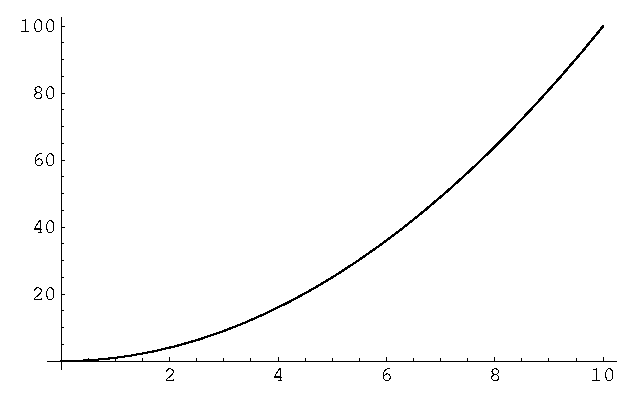
\includegraphics{plot.eps}
  \caption{%
    By default figures are not centered.
    This is a long caption to demonstrate that captions are single spaced.
  }
  \label{fi:not-centered}
\end{figure}

\Repeat{This is the second paragraph.}{10}

\begin{figure}[h]
  \centering
  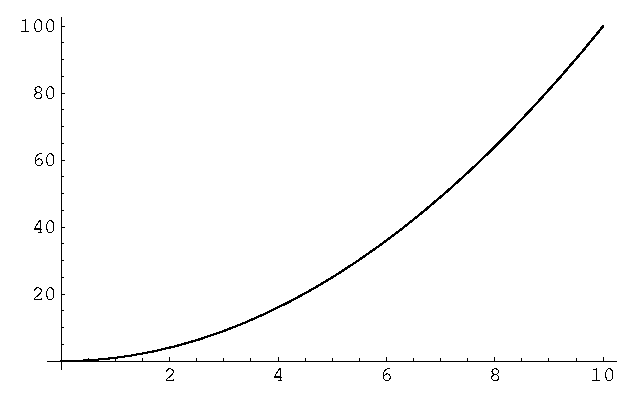
\includegraphics{plot.eps}
  \caption{Use {\tt \char'134centering\/} to center figures.}
  \label{fi:centered}
\end{figure}

\Repeat{This is the third paragraph.}{15}

\begin{figure}[h]
  \centering
  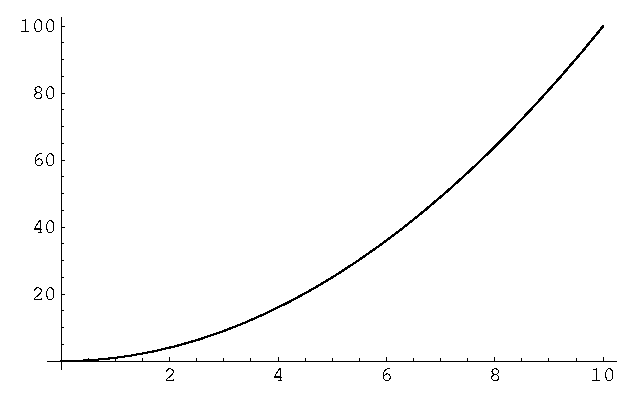
\includegraphics{plot.eps}
  \caption{This is another figuure.}
  \label{fi:another}
\end{figure}

\Repeat{This is the fourth paragraph.}{10}

\begin{figure}[h]
  \centering 
  \subfigure[First subcaption.]{\label{sf:two-parts-a}  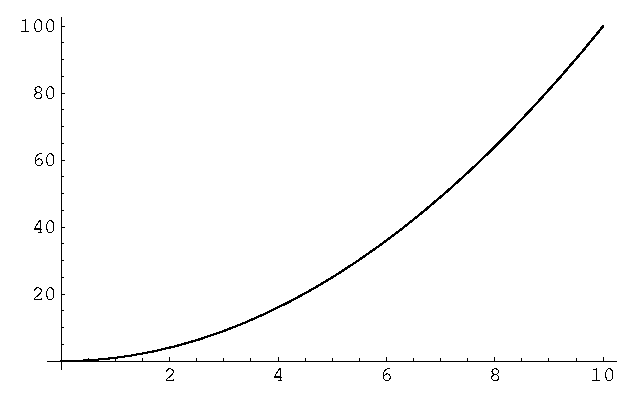
\includegraphics[width=0.3\textwidth]{plot.eps}}%
  \hskip 0.5truein
  \subfigure[Second subcaption.]{\label{sf:two-parts-b}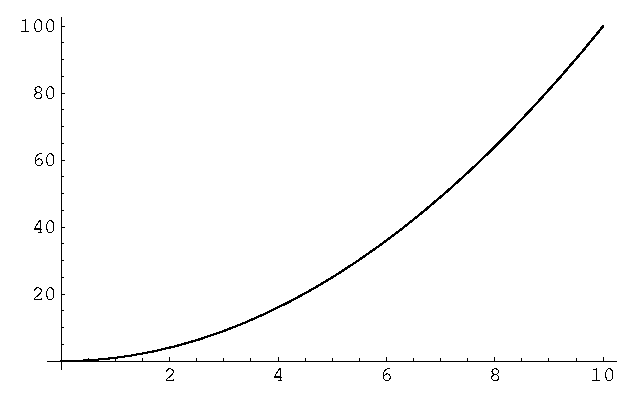
\includegraphics[width=0.3\textwidth]{plot.eps}}
  \caption{This figure has two parts.}
  \label{fi:two-parts}
\end{figure}

\Repeat{This is the fifth paragraph.}{10}

\begin{figure}[h]
  \centering
  \subfigure[First subcaption.]{\label{sf:four-parts-a}  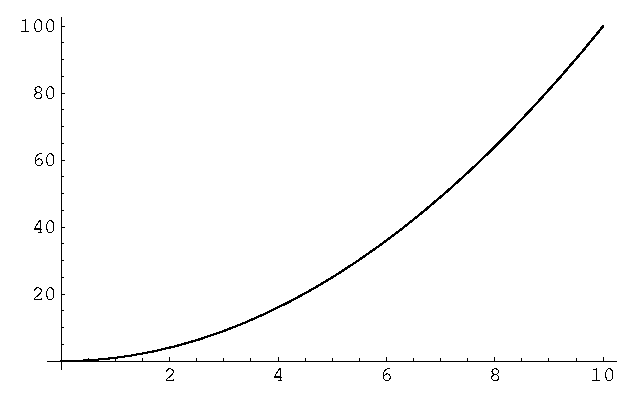
\includegraphics[width=0.3\textwidth]{plot.eps}}%
  \hskip 0.5truein
  \subfigure[Second subcaption.]{\label{sf:four-parts-b}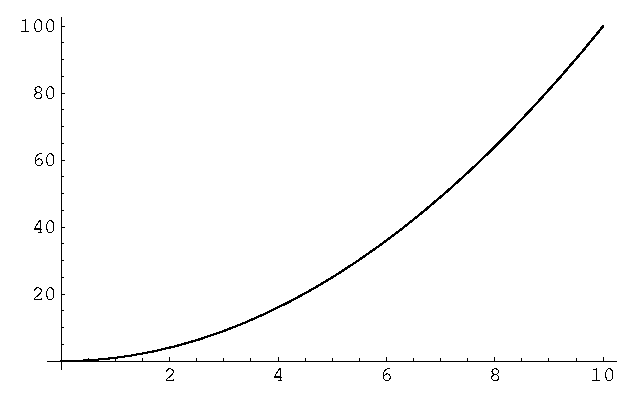
\includegraphics[width=0.3\textwidth]{plot.eps}}
  \subfigure[Third subcaption.]{\label{sf:four-parts-c}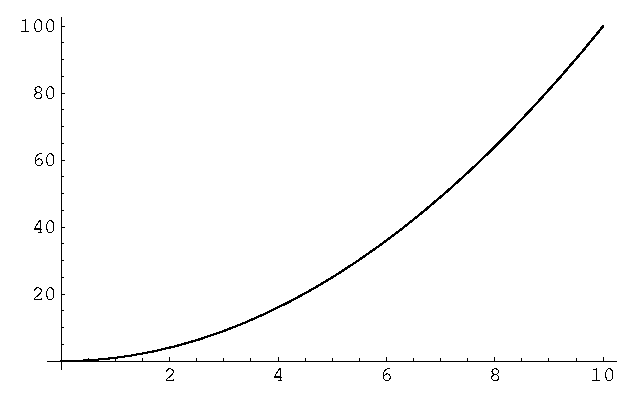
\includegraphics[width=0.3\textwidth]{plot.eps}}%
  \hskip 0.5truein
  \subfigure[Fourth subcaption.]{\label{sf:four-parts-d}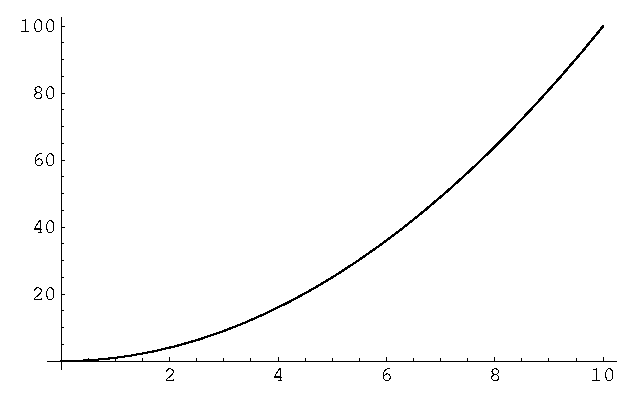
\includegraphics[width=0.3\textwidth]{plot.eps}}
  \caption{This figure has four parts.}
  \label{fi:four-parts}
\end{figure}

\Repeat{This is the sixth paragraph.}{10}

%%
%  THIS FILE DOES SOME UNUSUAL THINGS TO MAKE
%  IT EASIER TO DO DEMONSTRATIONS.  IT SHOULD
%  NOT BE USED AS AN EXAMPLE OF HOW TO PREPARE
%  A FILE.  SEE THE OUTPUT OF THIS FOR LATEX
%  INPUT AND OUTPUT EXAMPLES.
%




%
%  demo-mathematics.tex  2008-12-09  Mark Senn  http://engineering.purdue.edu/~mark
%

\chapter{Demonstrate Mathematics}

    % Use single spacing.
    \Baselinestretch{1}

    % You don't normally need this.
    \mbox{}

    \begin{verbatim}
% From _More Math Into LaTeX_, 4th Edition, page 152:
%     TeX uses $$ to open and close a displayed math environment.
%     In LaTeX, this may occassionally cause problems.  Don't do it.
\[
    E = mc^2
\]
    \end{verbatim}
% From _More Math Into LaTeX_, 4th Edition, page 152:
%     TeX uses $$ to open and close a displayed math environment.
%     In LaTeX, this may occassionally cause problems.  Don't do it.
\[
    E = mc^2
\]
    \vskip\baselineskip
    \hrule
    \vskip0.5\baselineskip
    \filbreak

    \begin{verbatim}
\begin{equation}
    E = mc^2
\end{equation}
    \end{verbatim}
\begin{equation}
    E = mc^2
\end{equation}
    \vskip\baselineskip
    \hrule
    \vskip0.5\baselineskip
    \filbreak

    \begin{verbatim}
% Mydefs.tex defines \be to be \begin{equation} and
% \ee to be \end{equation}.
\be
    E = mc^2
\ee
    \end{verbatim}
% Mydefs.tex defines \be to be \begin{equation} and
% \ee to be \end{equation}.
\be
    E = mc^2
\ee
    \vskip\baselineskip
    \hrule
    \vskip0.5\baselineskip
    \filbreak

    \begin{verbatim}
\be
    x = -\frac{b}{2a} \pm \frac{\sqrt{b^2 - 4ac}}{2a}
\ee
    \end{verbatim}
\be
    x = -\frac{b}{2a} \pm \frac{\sqrt{b^2 - 4ac}}{2a}
\ee
    \vskip\baselineskip
    \hrule
    \vskip0.5\baselineskip
    \filbreak

    \begin{verbatim}
% requires \usepackage{amsmath}; use align* for no equation number
\begin{align}
    a = {}& b + c\\
    x = {}& y + z
\end{align}
    \end{verbatim}
% requires \usepackage{amsmath}; use align* for no equation number
\begin{align}
    a = {}& b + c\\
    x = {}& y + z
\end{align}
    \vskip\baselineskip
    \hrule
    \vskip0.5\baselineskip
    \filbreak

    \begin{verbatim}
\[
    Z = \left(
        \begin{array}{cc}
            a& b\\
            c& d
        \end{array}
    \right)
\]
    \end{verbatim}
\[
    Z = \left(
        \begin{array}{cc}
            a& b\\
            c& d
        \end{array}
    \right)
\]
    \vskip\baselineskip
    \hrule
    \vskip0.5\baselineskip
    \filbreak

    \begin{verbatim}
\begin{equation}
    \begin{split}
        a = {}& b + c\\
            {}& + d + e
    \end{split}      
\end{equation}
    \end{verbatim}
\begin{equation}
    \begin{split}
        a = {}& b + c\\
            {}& + d + e
    \end{split}      
\end{equation}
    \vskip\baselineskip
    \hrule
    \vskip0.5\baselineskip
    \filbreak

    \begin{verbatim}
\be
    (\cos x)^2 + (\sin x)^2 = 1
\ee
    \end{verbatim}
\be
    (\cos x)^2 + (\sin x)^2 = 1
\ee
    \vskip\baselineskip
    \hrule
    \vskip0.5\baselineskip
    \filbreak

    \begin{verbatim}
If $X = \cos x$ and $Y = \sin x$ then $X^2 + Y^2 = 1$.
    \end{verbatim}
If $X = \cos x$ and $Y = \sin x$ then $X^2 + Y^2 = 1$.
    \vskip\baselineskip
    \hrule
    \vskip0.5\baselineskip
    \filbreak

%%
%  demo-multicols.tex  2007-03-19  Mark Senn  http://www.ecn.purdue.edu/~mark
%
%  Demonstrate multicols.
%
%  The multicols package must be loaded for this to work.
%  To load the multicols package put
%      \usepackage{multicols}
%  between the "\documentclass" and "\begin{document}" commands.
%

\chapter{Demonstrate Multicols}

% Put this amount of space between the columns.
\setlength{\columnsep}{0.5truein}

% Separate the columns with a vertical rule this wide.
\setlength{\columnseprule}{0.4pt}

\Repeat{This is one column.}{25}

\begin{multicols}{2}
\Repeat{This is two columns.}{25}
\end{multicols}

\begin{multicols}{3}
\Repeat{This is three columns.}{25}
\end{multicols}

\begin{multicols}{4}
\Repeat{This is four columns.}{25}
\end{multicols}

\begin{multicols}{5}
\Repeat{This is five columns.}{25}
\end{multicols}

%%
%  demo-tables.tex  2014-08-08  Mark Senn
%
%  Demonstrate how to do tables.
%

\chapter{Demonstrate Tables}

% \newlength{\ta}
% \newlength{\tb}
% \newlength{\tc}
% 
% \settowidth{\ta}{\vbox{\hbox{Money}\hbox{Market}}}
% \settowidth{\tb}{\vbox{\hbox{Stocks}\hbox{and}\hbox{Bonds}}}
% \settowidth{\tc}{\vbox{\hbox{Money}\hbox{Market}\hbox{and}\hbox{Stocks}}}
% 
% {
%     \renewcommand{\baselinestretch}{1}
%     \begin{table}
%       \caption{%
%         \hfil Allocation of the IRA and Keogh Wealth\hfil\break
%         \mbox{}\hfil for Investors With or Without Brokerage Accounts\hfil
%       }
%       \label{tab:ira}
%       \begin{center}
%         \begin{tabular}%
%           {%
%             |%
%             c%
%             |%
%             >{\centering\hspace{0pt}}m{\the\ta}%  Money Market
%             |%
%             c%                                    Stocks 
%             |%
%             c%                                    Bonds
%             |%
%             c%                                    Diversified
%             |%
%             >{\centering\hspace{0pt}}m{\the\tb}%  Stocks and Bonds
%             |%
%             >{\centering\hspace{0pt}}m{\the\tc}%  Money Market and Stocks
%             |%
%             c%                                    Others
%             |%
%           }
%           \hline
%           IMP&
%             Money Market&
%             Stocks&
%             Bonds&
%             Diversified&
%             Stocks and Bonds&
%             Money Market and Stocks&
%             Others\tabularnewline
%           \hline
%           1& 14.19\%& 57.71\%& 12.21\%& 4.50\%& 7.36\%& 3.04\%& 0.99\%\tabularnewline \hline
%           2& 14.08\%& 58.18\%& 12.32\%& 4.44\%& 7.30\%& 2.80\%& 0.88\%\tabularnewline \hline
%           3 &14.26\%& 58.09\%& 12.27\%& 4.50\%& 7.19\%& 2.75\%& 0.94\%\tabularnewline \hline
%           4 &13.94\%& 58.11\%& 12.14\%& 4.78\%& 7.35\%& 2.68\%& 0.99\%\tabularnewline \hline
%           5 &13.92\%& 58.13\%& 11.93\%& 4.56\%& 7.60\%& 2.98\%& 0.88\%\tabularnewline \hline
%         \end{tabular}
%       \end{center}
%       This table presents the allocations of the wealth in the IRA
%       and Keogh accounts in various asset classes.
%       Results from each set of imputed data are presented here.
%       The first column lists the number of the imputations,
%       and rest of the columns lists various allocations.
%       Entrees under each asset class show the percentage of investors
%       who have most of their IRA
%       and Keogh wealth invested in that particular asset class.
%       The asset class Diversified
%       includes stocks,
%       bonds,
%       and money market investments.
%       The asset class Others
%       include investments in various life insurance products,
%       annuities,
%       real estate, etc.
%       \medskip
%     \footnotesize SOURCE: Survey of Consumer Finances,
%     2001,
%     Federal Reserve Board,
%     USA.\par
%   \end{table}
% }

Here is a really simple table.

% "h" means put table here---don't let it float to top or bottom of page
\begin{table}[h]
  \caption{American Presidents}
  \begin{center}
    \begin{tabular}{rl}
      \bf Number& \bf Name\\
      1& George Washington\\
      2& John Adams\\
      3& Thomas Jefferson\\
    \end{tabular}
  \end{center}
  \label{ta:American-Presidents}
\end{table}

There are 72.27 points per inch.
I like to put 2 points of vertical space between the heading
(Number Name)
and the first line
(1 George Washington)
of the table.

\begin{table}[h]
  \caption{American Presidents with 2pt vertical space after heading}
  \begin{center}
    \begin{tabular}{rl}
      \bf Number& \bf Name\\[2pt]  % put 2pt vertical space after this line
      1& George Washington\\
      2& John Adams\\
      3& Thomas Jefferson\\
    \end{tabular}
  \end{center}
  \label{ta:American-Presidents-with-2pt}
\end{table}

\LaTeX\ can print horizontal and vertical rules in tables.
I don't like the way this looks.

\begin{table}[h]
  \caption{American Presidents with horizontal and vertical lines}
  \begin{center}
    % "|" prints a vertical rule, "c" means center
    \begin{tabular}{|c|l|}
      % "\hline" prints a horizontal rule
      \hline
      \bf\#& \bf Name\\
      \hline
      1& George Washington\\
      \hline
      2& John Adams\\
      \hline
      3& Thomas Jefferson\\
      \hline
    \end{tabular}
  \end{center}
  \label{ta:American-Presidents-with-horizontal}
\end{table}

\newpage

Here is a more complicated table.

\begin{table}[h]
  \caption{C Bitwise Operators}
  \begin{center}
    % "|" prints a vertical rule, "c" means center
    \begin{tabular}{cccc}
      \bf A& \bf B& \bf A$|$B& \bf A\&B\\[2pt]
      0& 0& 0& 0\\
      0& 1& 1& 0\\
      1& 0& 1& 0\\
      1& 1& 1& 1\\
    \end{tabular}
  \end{center}
  \label{ta:C-Bitwise}
\end{table}

You can use Plain \TeX's \verb+\halign+ command to make tables also.
If you can't do a complicated table using \LaTeX\ commands
you may want to try using Plain \TeX\ commands.
\LaTeX's table making commands use Plain \TeX\ commands.

\begin{table}[h]
  \caption{American Presidents using {\tt\char'134 halign}}
  \hbox to \textwidth{\hss\vbox{\halign{%
    \strut #&      % 0. \strut
    \hfil#\qquad&  % 1. Number
    #\hfil\cr      % 2. Name
    %
    & \bf Number& \bf Name\cr
    \noalign{\vskip 2pt}
    & 1& George Washington\cr
    & 2& John Adams\cr
    & 3& Thomas Jefferson\cr
  }}\hss}
  \label{ta:American-Presidents-using}
\end{table}

The next page shows how to do a table that is too long to fit on one page.

\newpage

% This is loosely based on page 106 of _A Guide to LaTeX_, third edition,
% by Helmut Kopka and Patrick W. Daly.
\begin{longtable}{|l|l|}
    \caption{State Abbreviations}\\
    \hline
    State& Abbreviation\\
    \hline
  \endfirsthead
    \caption[]{\emph{continued}}\\
    \hline
    State& Abbreviation\\
    \hline
  \endhead
    \hline
    \multicolumn{2}{r}{\emph{continued on next page}}
  \endfoot
    \hline
  \endlastfoot
  Alabama& AL\\
  Alaska& AK\\
% American Samoa& AS\\
  Arizona& AZ\\
  Arkansas& AR\\
% Armed Forces Europe& AE\\
% Armed Forces Pacific& AP\\
% Armed Forces the Americas& AA\\
  California& CA\\
  Colorado& CO\\
  Connecticut& CT\\
  Delaware& DE\\
% District of Columbia& DC\\
% Federated States of Micronesia& FM\\
  Florida& FL\\
  Georgia& GA\\
% Guam& GU\\
  Hawaii& HI\\
  Idaho& ID\\
  Illinois& IL\\
  Indiana& IN\\
  Iowa& IA\\
  Kansas& KS\\
  Kentucky& KY\\
  Louisiana& LA\\
  Maine& ME\\
% Marshall Islands& MH\\
  Maryland& MD\\
  Massachusetts& MA\\
  Michigan& MI\\
  Minnesota& MN\\
  Mississippi& MS\\
  Missouri& MO\\
  Montana& MT\\
  Nebraska& NE\\
  Nevada& NV\\
  New Hampshire& NH\\
  New Jersey& NJ\\
  New Mexico& NM\\
  New York& NY\\
  North Carolina& NC\\
  North Dakota& ND\\
% Northern Mariana Islands& MP\\
  Ohio& OH\\
  Oklahoma& OK\\
  Oregon& OR\\
  Pennsylvania& PA\\
% Puerto Rico& PR\\
  Rhode Island& RI\\
  South Carolina& SC\\
  South Dakota& SD\\
  Tennessee& TN\\
  Texas& TX\\
  Utah& UT\\
  Vermont& VT\\
% Virgin Islands& VI\\
  Virginia& VA\\
  Washington& WA\\
  West Virginia& WV\\
  Wisconsin& WI\\
  Wyoming& WY\\
\end{longtable}

\newcommand{\cbackslash}{\char'134}
\newcommand{\copencurly}{\char'173}
\newcommand{\cclosecurly}{\char'175}

\newlength{\twidth}
\newlength{\theight}

\setlength{\twidth}{\textwidth}
\setlength{\theight}{\textheight}

\begin{sidewaystable}
  % The following two lines compensate for what I think is a bug.
  \setlength{\textwidth}{\theight}
  \setlength{\textheight}{\twidth}
  \caption{%
    sidewaystable
    {\tt\cbackslash begin\copencurly tabular\cclosecurly\/}%
    \ldots
    {\tt\cbackslash end\copencurly tabular\cclosecurly\/}%
  }
  \begin{center}
    \begin{tabular}{rl}
      \bf Number& \bf Name\\[2pt]  % put 2pt vertical space after this line
      1& George Washington\\
      2& John Adams\\
      3& Thomas Jefferson\\
    \end{tabular}
  \end{center}
\end{sidewaystable}

\begin{sidewaystable}
  % The following two lines compensate for what I think is a bug.
  \setlength{\textwidth}{\theight}
  \setlength{\textheight}{\twidth}
  \caption{%
    sidewaystable
    {\tt\cbackslash halign\copencurly}\ldots{\tt\cclosecurly\/} table%
  }
  \hbox to \textwidth{\hss\vbox{\halign{%
    \strut #&      % 0. \strut
    \hfil#\qquad&  % 1. Number
    #\hfil\cr      % 2. Name
    %
    & \bf Number& \bf Name\cr
    \noalign{\vskip 2pt}
    & 1& George Washington\cr
    & 2& John Adams\cr
    & 3& Thomas Jefferson\cr
  }}\hss}
\end{sidewaystable}

%\newlength{\ta}
%\settowidth{\ta}{\vbox{\hbox{Money}\hbox{Market}}}
%\newlength{\tb}
%\settowidth{\tb}{\vbox{\hbox{Stocks}\hbox{and}\hbox{Bonds}}}
%\newlength{\tc}
%\settowidth{\tc}{\vbox{\hbox{Money}\hbox{Market}\hbox{and}\hbox{Stocks}}}
%
%  {\renewcommand{\baselinestretch}{1}
%\begin{table}
%  \caption{\hfil Allocation of the IRA and Keogh Wealth\hfil\break\mbox{}\hfil for Investors With or Without Brokerage Accounts\hfil}
%  \label{tab:ira}
%  \begin{center}
%    \begin{tabular}%
%      {%
%        |%
%        c%
%        |%
%        >{\centering\hspace{0pt}}m{\the\ta}%  Money Market
%        |%
%        c%                                    Stocks 
%        |%
%        c%                                    Bonds
%        |%
%        c%                                    Diversified
%        |%
%        >{\centering\hspace{0pt}}m{\the\tb}%  Stocks and Bonds
%        |%
%        >{\centering\hspace{0pt}}m{\the\tc}%  Money Market and Stocks
%        |%
%        c%                                    Others
%        |%
%      }
%      \hline
%      IMP&
%        Money Market&
%        Stocks&
%        Bonds&
%        Diversified&
%        Stocks and Bonds&
%        Money Market and Stocks&
%        Others\tabularnewline
%      \hline
%      1& 14.19\%& 57.71\%& 12.21\%& 4.50\%& 7.36\%& 3.04\%& 0.99\%\tabularnewline \hline
%      2& 14.08\%& 58.18\%& 12.32\%& 4.44\%& 7.30\%& 2.80\%& 0.88\%\tabularnewline \hline
%      3 &14.26\%& 58.09\%& 12.27\%& 4.50\%& 7.19\%& 2.75\%& 0.94\%\tabularnewline \hline
%      4 &13.94\%& 58.11\%& 12.14\%& 4.78\%& 7.35\%& 2.68\%& 0.99\%\tabularnewline \hline
%      5 &13.92\%& 58.13\%& 11.93\%& 4.56\%& 7.60\%& 2.98\%& 0.88\%\tabularnewline \hline
%    \end{tabular}
%  \end{center}
%  This table presents the allocations of the wealth in the IRA
%  and Keogh accounts in various asset classes.
%  Results from each set of imputed data are presented here.
%  The first column lists the number of the imputations,
%  and rest of the columns lists various allocations.
%  Entrees under each asset class show the percentage of investors
%  who have most of their IRA
%  and Keogh wealth invested in that particular asset class.
%  The asset class Diversified
%  includes stocks,
%  bonds,
%  and money market investments.
%  The asset class Others
%  include investments in various life insurance products,
%  annuities,
%  real estate, etc.
%  \medskip
%  \footnotesize SOURCE: Survey of Consumer Finances,
%  2001,
%  Federal Reserve Board,
%  USA.\par
%\end{table}
%  }


%%
%  demo-text.tex  2007-07-17  Mark Senn  http://engineering.purdue.edu/~mark
%

\chapter{Demonstrate Text}

% Use single spacing.
\Baselinestretch{1}

% You don't normally need this.
\mbox{}


%\vbox{
\begin{verbatim}
This is a sentence.
This is a sentence.
This is a sentence.
This is a sentence.
This is a sentence.

This is a sentence.
This is a sentence.
This is a sentence.
This is a sentence.
This is a sentence.
\end{verbatim}
This is a sentence.
This is a sentence.
This is a sentence.
This is a sentence.
This is a sentence.

This is a sentence.
This is a sentence.
This is a sentence.
This is a sentence.
This is a sentence.
\vskip\baselineskip
\hrule
%}
\vskip0.5\baselineskip
\filbreak

%\vbox{
\begin{verbatim}
From \verb+http://www.biblegateway.com/passage/?book_id=1&chapter=1&version=50+:

\begin{quote}
    1 In the beginning God created the heavens and the earth.
    2 The earth was without form,
    and void;
    and darkness was on the face of the deep.
    And the Spirit of God was hovering over the face of the waters.

    3 Then God said,``Let there be light'';
    and there was light.
    4 And God saw the light,
    that it was good;
    and God divided the light from the darkness.
    5 God called the light Day,
    and the darkness He called Night.
    So the evening and the morning were the first day. 
\end{quote}
\end{verbatim}
From \verb+http://www.biblegateway.com/passage/?book_id=1&chapter=1&version=50+:

\begin{quote}
    1 In the beginning God created the heavens and the earth.
    2 The earth was without form,
    and void;
    and darkness was on the face of the deep.
    And the Spirit of God was hovering over the face of the waters.

    3 Then God said,``Let there be light'';
    and there was light.
    4 And God saw the light,
    that it was good;
    and God divided the light from the darkness.
    5 God called the light Day,
    and the darkness He called Night.
    So the evening and the morning were the first day. 
\end{quote}
\vskip\baselineskip
\hrule
%}
\vskip0.5\baselineskip
\filbreak

%\vbox{
\begin{verbatim}
\begin{description}
    \item[apple]
        A red fruit.
    \item[banana]
        A yellow fruit.
        This sentence is to make the entry longer so you can see what happens.
        This sentence is to make the entry longer so you can see what happens.
    \item[cherry]
        A red friut.
\end{description}
\end{verbatim}
\begin{description}
    \item[apple]
        A red fruit.
    \item[banana]
        A yellow fruit.
        This sentence is to make the entry longer so you can see what happens.
        This sentence is to make the entry longer so you can see what happens.
    \item[cherry]
        A red friut.
\end{description}
\vskip\baselineskip
\hrule
%}
\vskip0.5\baselineskip
\filbreak

%\vbox{
\begin{verbatim}
\begin{enumerate}
    \item apple
    \item banana
        This sentence is to make the entry longer so you can see what happens.
        This sentence is to make the entry longer so you can see what happens.
    \item cherry
\end{enumerate}
\end{verbatim}
\begin{enumerate}
    \item apple
    \item banana
        This sentence is to make the entry longer so you can see what happens.
        This sentence is to make the entry longer so you can see what happens.
    \item cherry
\end{enumerate}
\vskip\baselineskip
\hrule
%}
\vskip0.5\baselineskip
\filbreak


%\vbox{
\begin{verbatim}
\begin{itemize}
    \item apple
    \item banana
        This sentence is to make the entry longer so you can see what happens.
        This sentence is to make the entry longer so you can see what happens.
    \item cherry
\end{itemize}
\end{verbatim}
\begin{itemize}
    \item apple
    \item banana
        This sentence is to make the entry longer so you can see what happens.
        This sentence is to make the entry longer so you can see what happens.
    \item cherry
\end{itemize}
\vskip\baselineskip
\hrule
%}
\vskip0.5\baselineskip
\filbreak

%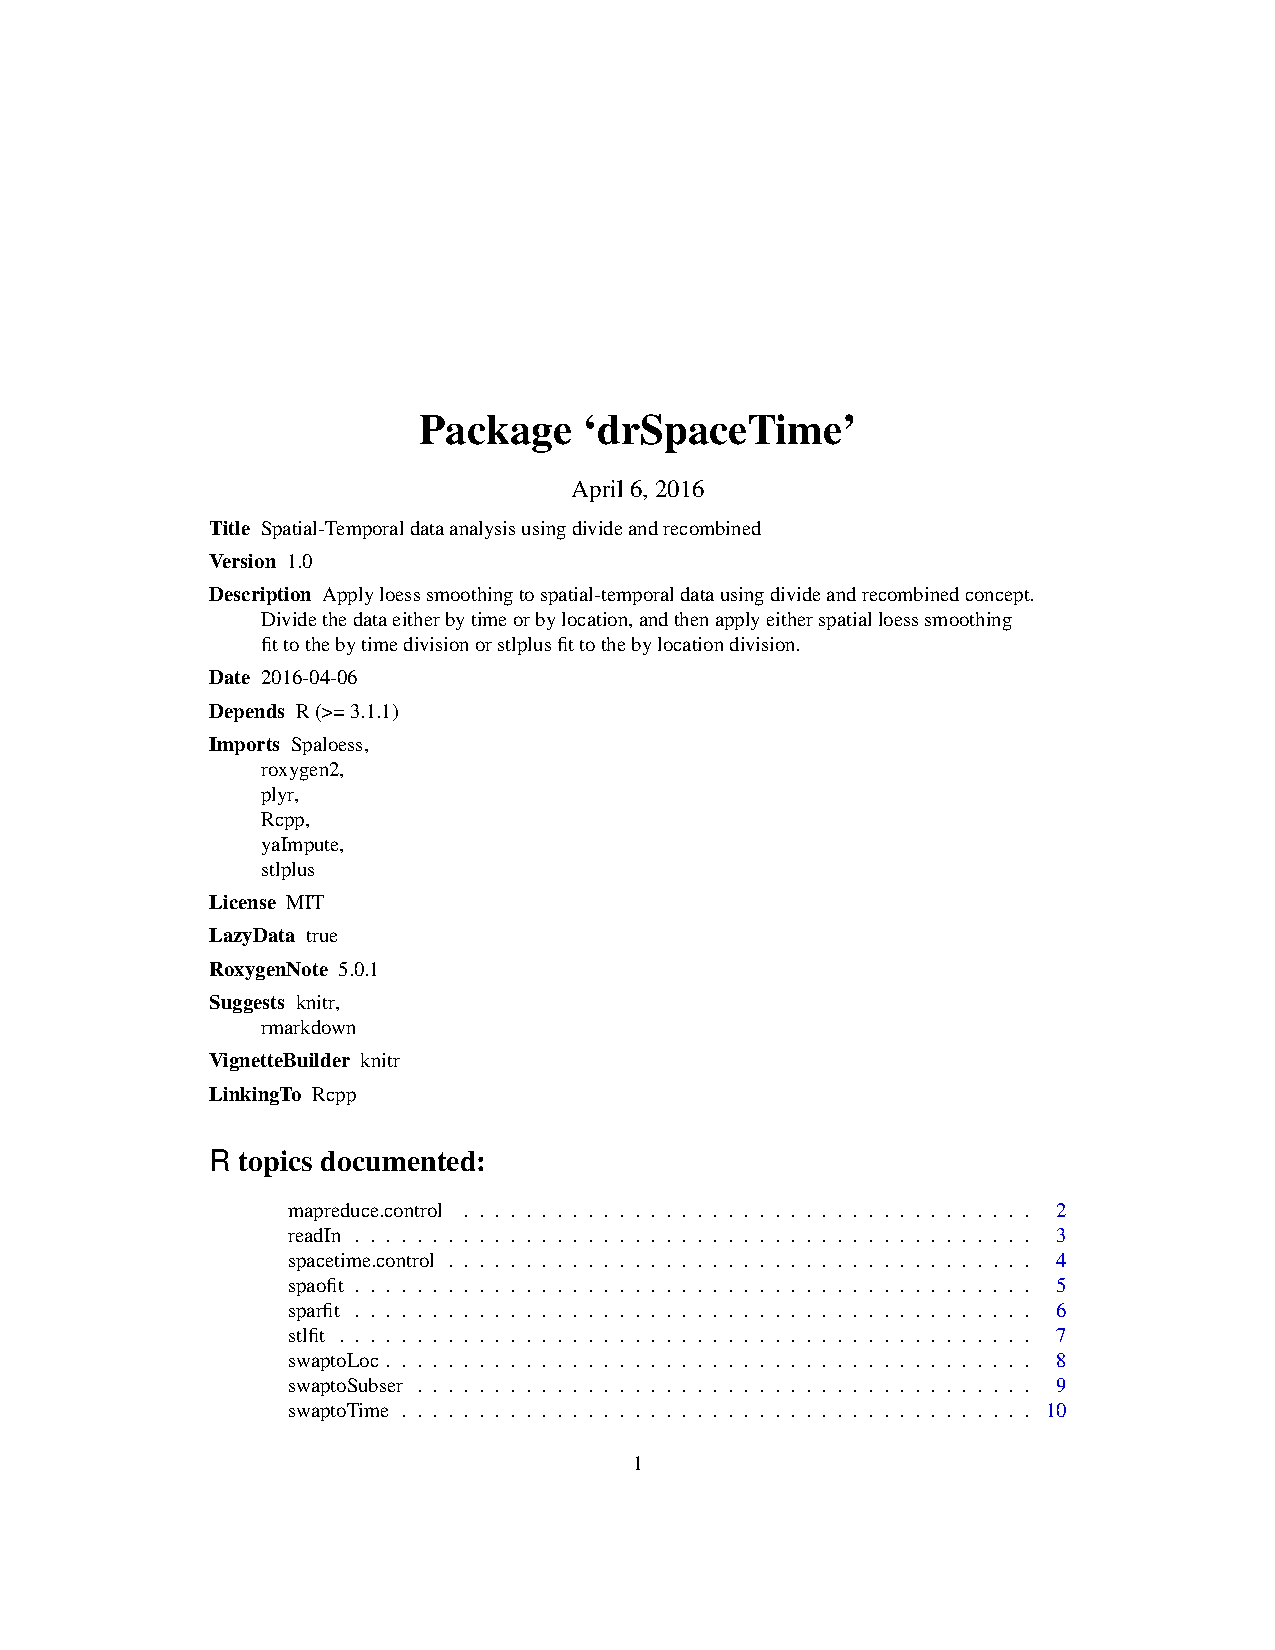
\includepdf[pages={-}]{drSpaceTime.pdf}

%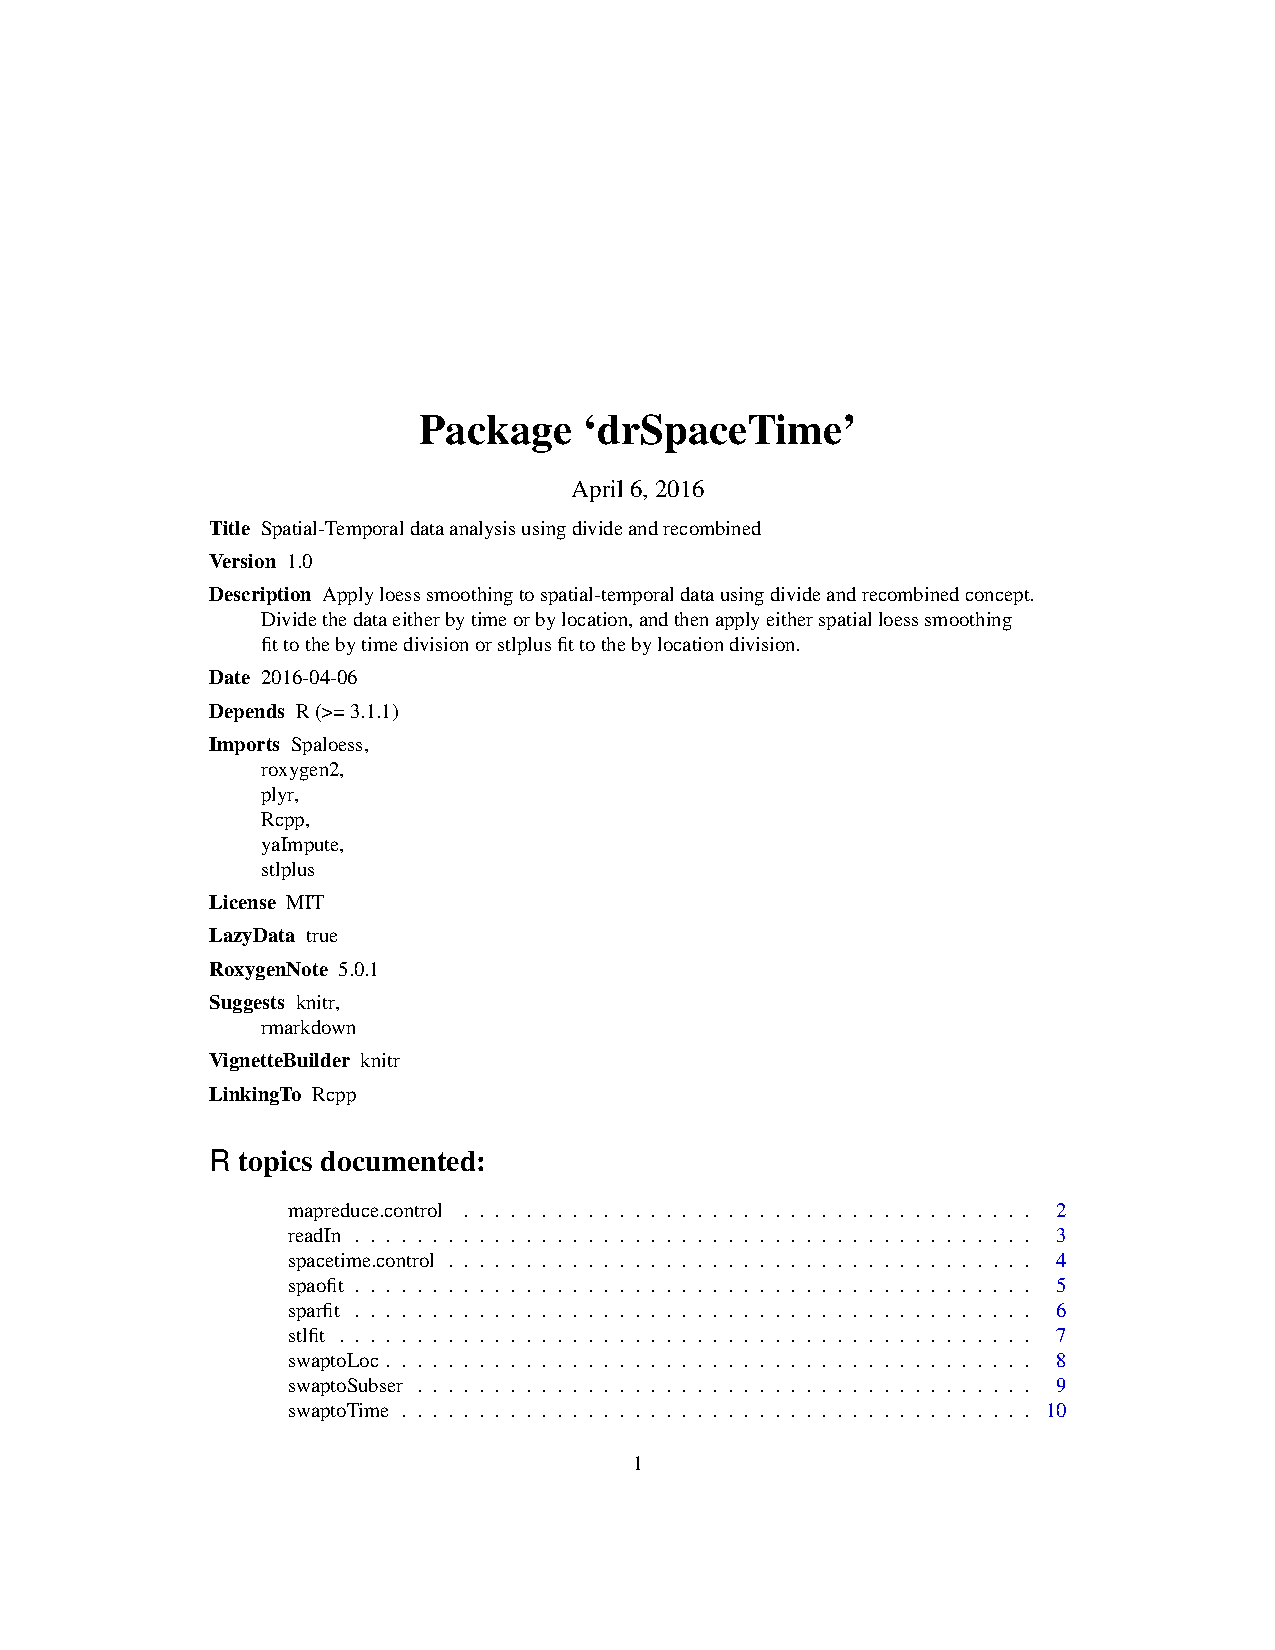
\includepdf[pages=-,scale=.8,pagecommand={}]{drSpaceTime}



\fancypage{\fboxrule=0.5pt\fboxsep=1mm\fbox}{}

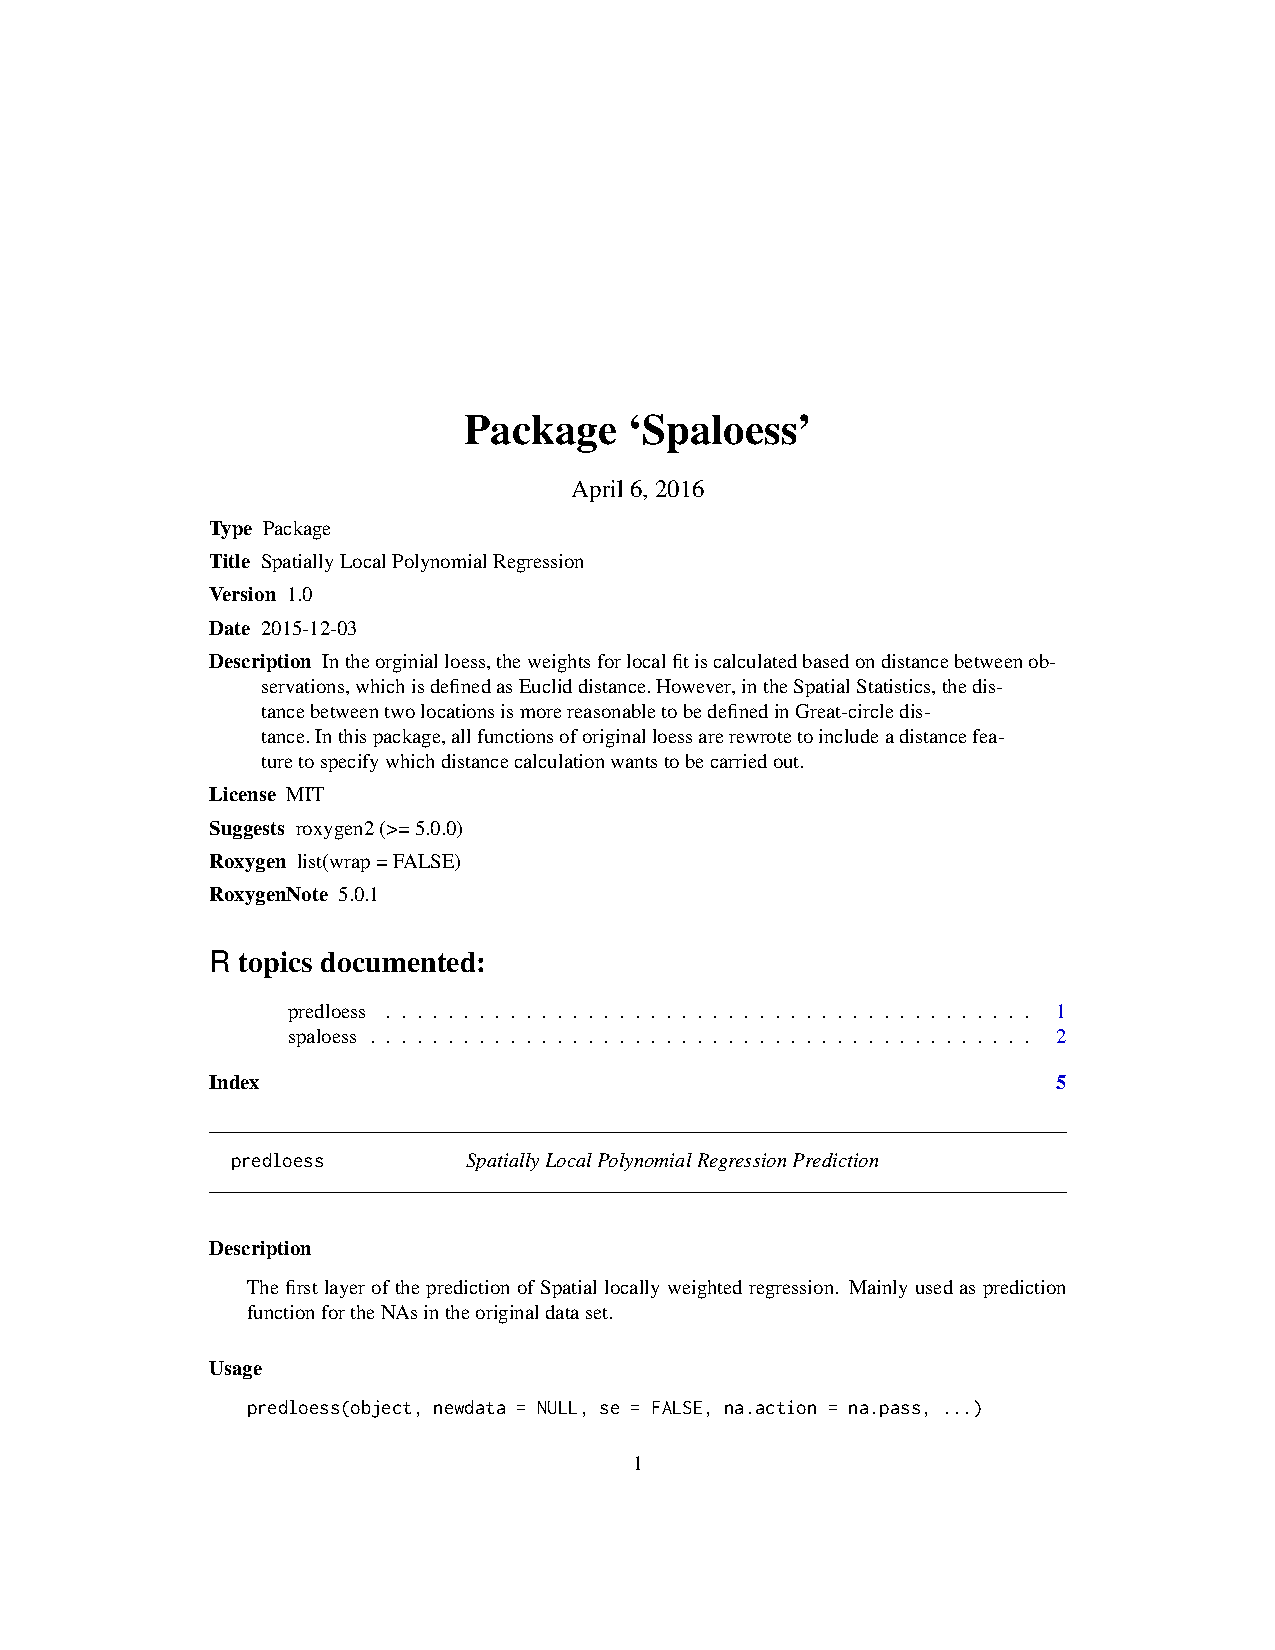
\includepdf[pages=-, pagecommand={},scale=1]{Spaloess.pdf}
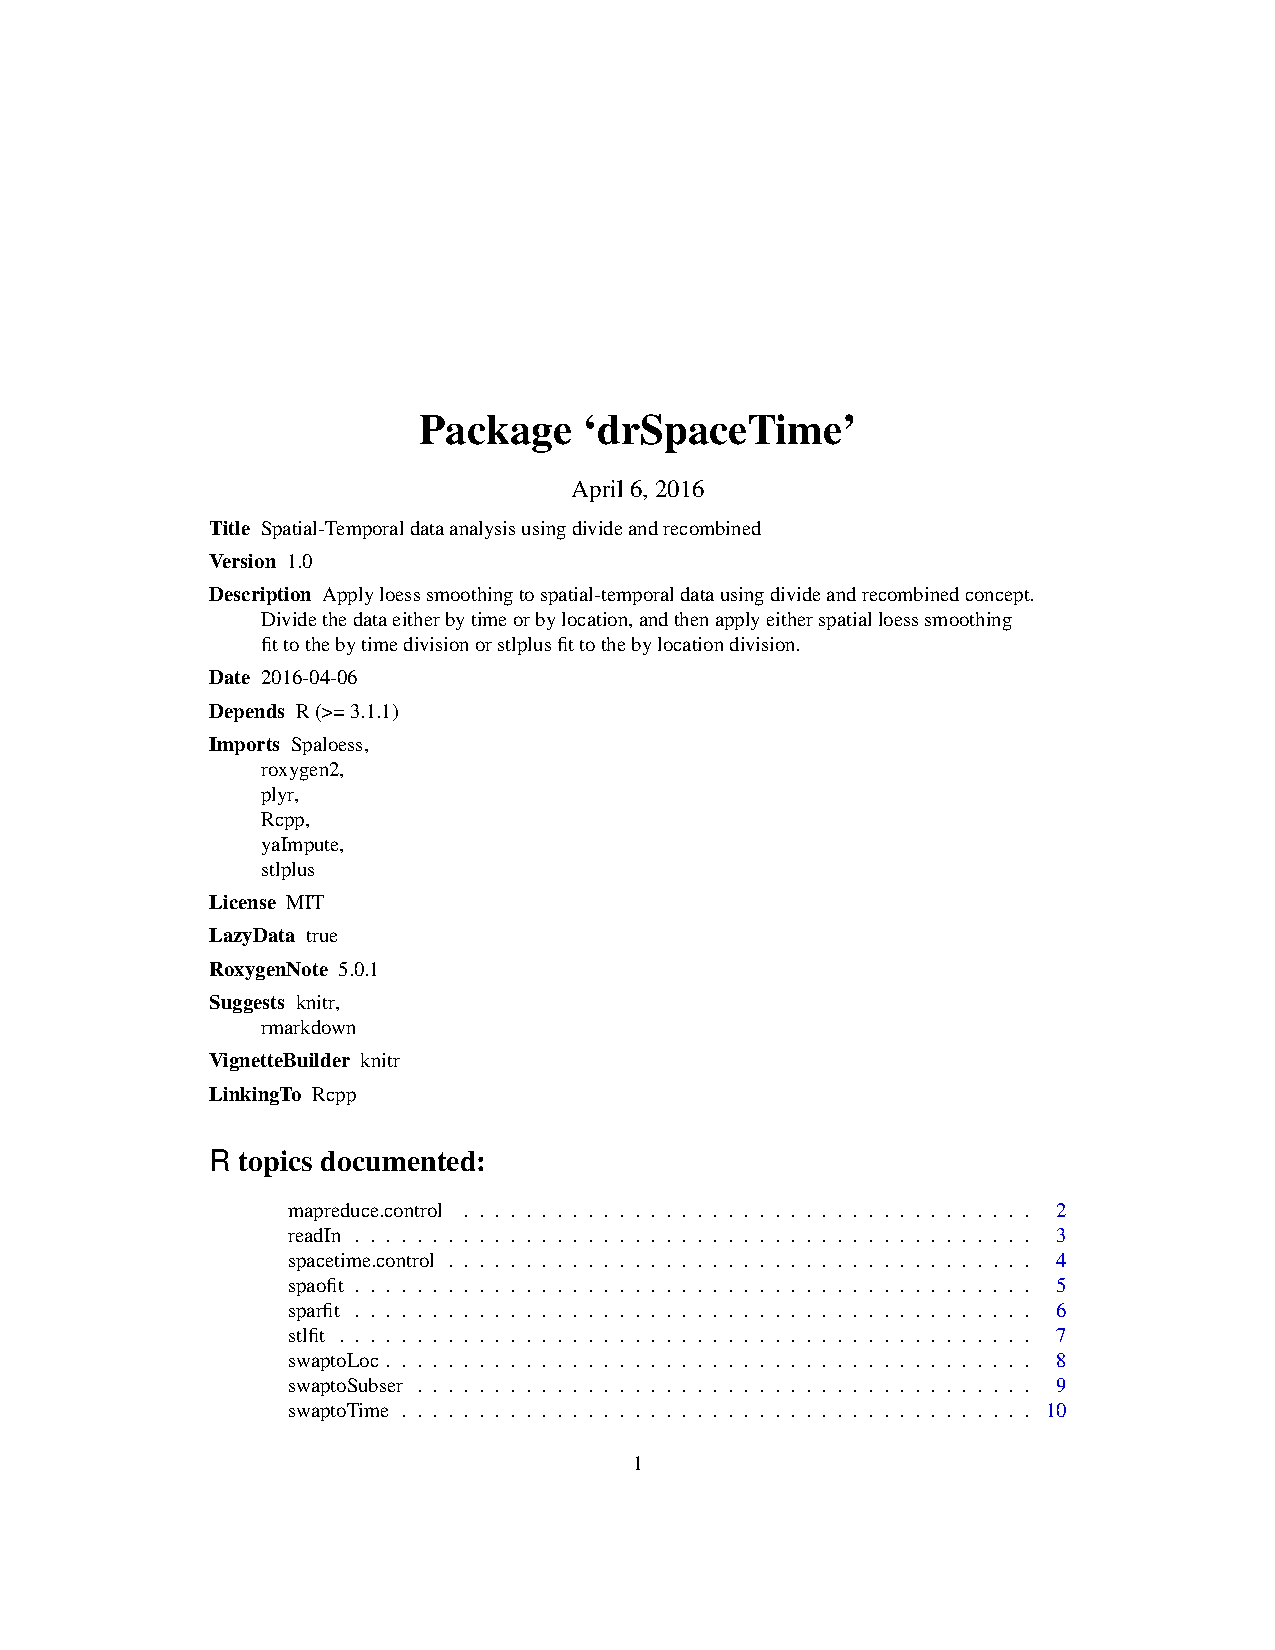
\includepdf[pages=-, pagecommand={},scale=1]{drSpaceTime.pdf}


% Notes and footnotes are optional.
% Reference: TM2006 page 34.
% I have not implemented this yet.  Mark Senn 2002-06-03
%%\include{notes}

% A vita is optional for masters theses
% and required for doctoral dissertations.
% Reference: TM2006 page 13.
% CHANGE NEXT LINE?
%
%  vita.tex   2003.07.23  14:59:33   Mark Senn <mds@purdue.edu>
%
%  This is the vita for a simple, example thesis.
%
%  A vita is required only in a doctoral dissertation.
%

\begin{vita}

Xiaosu Tong was born in Xichang, Sichuan, China in 1988. He earned his B.S. in 
Information and Calculation Science at College of Science, Shenyangjianzhu 
University, China in 2010. Then he pursued his M.S. in Applied Statistics at Purdue
University, Indiana in 2012. His academic interests include exploratory data 
analysis, data visualization, time series, and statistical computation with
large and complex data.

\end{vita}


\end{document}

% LaTeX won't read after the \end{document} command.
% You can put notes to yourself or LaTeX input not
% ready for use here if you'd like.
